\documentclass[10pt,twocolumn,letterpaper]{article}

\usepackage{cvpr}
\usepackage{times}
\usepackage{epsfig}
\usepackage{graphicx}
\usepackage{amsmath}
\usepackage{amssymb}
\usepackage{verbatim}

% Include other packages here, before hyperref.

% If you comment hyperref and then uncomment it, you should delete
% egpaper.aux before re-running latex.  (Or just hit 'q' on the first latex
% run, let it finish, and you should be clear).
\usepackage[pagebackref=true,breaklinks=true,letterpaper=true,colorlinks,bookmarks=false]{hyperref}


\cvprfinalcopy % *** Uncomment this line for the final submission

\def\cvprPaperID{20} % *** Enter the CVPR Paper ID here
\def\httilde{\mbox{\tt\raisebox{-.5ex}{\symbol{126}}}}

% Pages are numbered in submission mode, and unnumbered in camera-ready
\ifcvprfinal\pagestyle{empty}\fi
\begin{document}

%%%%%%%%% TITLE
%\title{Utilizing Physical Avatars in a Projector-Camera Tangible User Interface \\ to Enhance Interaction and Engagement}

\title {Physical Avatars in a Projector-Camera Tangible User Interface 
\\  Enhance Quantitative Simulation Analysis and Engagement}

\author{Joshua Nasman\\
Rensselaer Polytechnic Institute\\
{\tt\small nasmaj@cs.rpi.edu}\\
% For a paper whose authors are all at the same institution,
% omit the following lines up until the closing ``}''.
% Additional authors and addresses can be added with ``\and'',
% just like the second author.
% To save space, use either the email address or home page, not both
\and
Barbara Cutler\\
Rensselaer Polytechnic Institute\\
{\tt\small cutler@cs.rpi.edu}\\
}


\maketitle
% \thispagestyle{empty}

%%%%%%%%% ABSTRACT
\begin{abstract}
\vspace{-0.1in}
%
We present an augmented reality environment for the visualization of
architectural daylighting simulations.  The new visualizations focus
the users' attention on the problematic aspects of a building design.
Architectural design is a task particularly well suited for Tangible
User Interfaces (TUIs).  
The user physically constructs a scale model of the building, a
lighting simulation is then performed on this space, and then the
simulation results are projected into the physical model by a set of
calibrated projectors.
A user study of an earlier version of the system revealed that users
lacked accurate quantitative information about the propagation of
natural light within architectural spaces and had difficulties
identifying and reasoning about areas of over-illumination,
under-illumination, and glare.  This was our motivation for two
important additions to the system: physical avatar tokens within the
physical scale model to specify areas of interest for glare and false
color visualizations.  We render viewpoints from the perspective of
each avatar and indicate glare for each viewpoint.  To provide users
with an additional way to minimize glare and provide visual interest,
we introduce new complex and interesting shading materials.
These features illustrated in our tool create a more immersive and
educational experience for novice and experienced designers.
\vspace{-0.15in}
\end{abstract}

\begin{figure*}[t]
%\newcommand{\picheight}{2.57in}
\newcommand{\picheight}{2.48in}
\newcommand{\picheightb}{1.85in}
\resizebox{!}{\picheight}{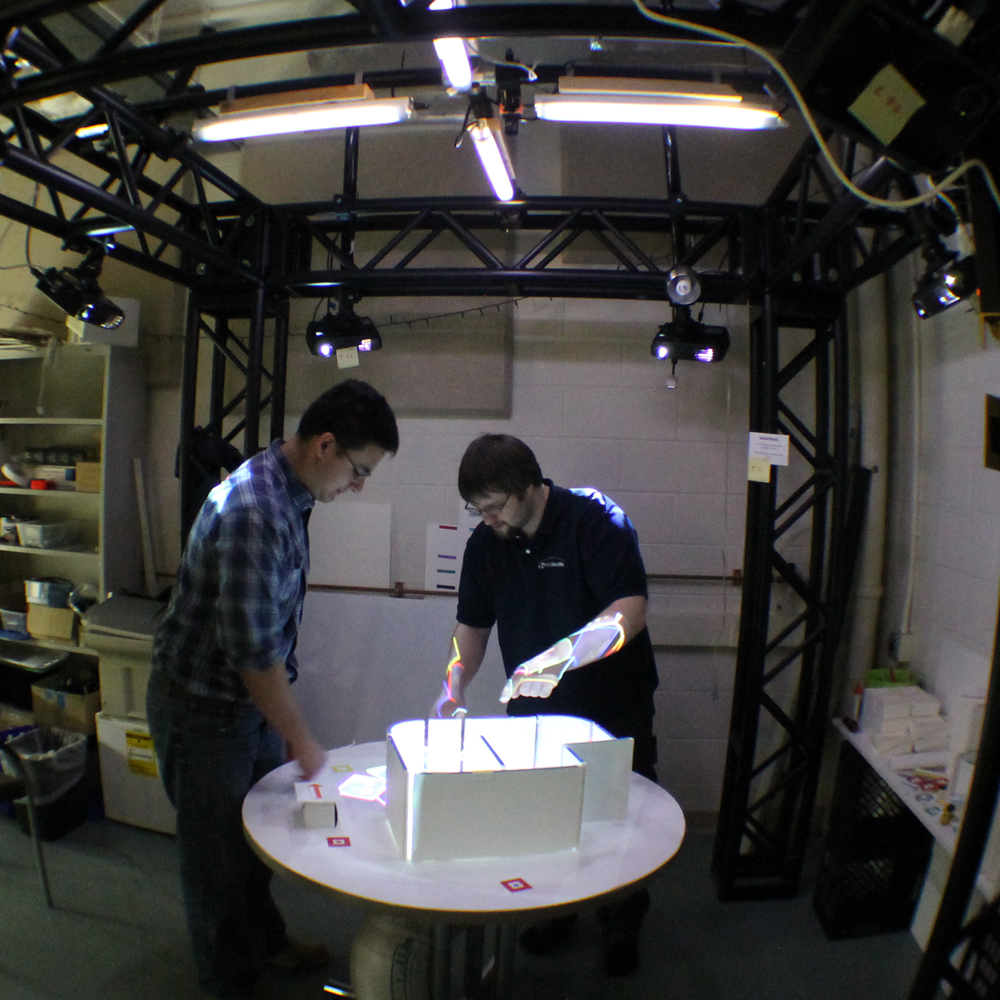
\includegraphics{photos/ian_matt_contraption_frame.jpg}}%
\hfill
%\resizebox{!}{\picheight}{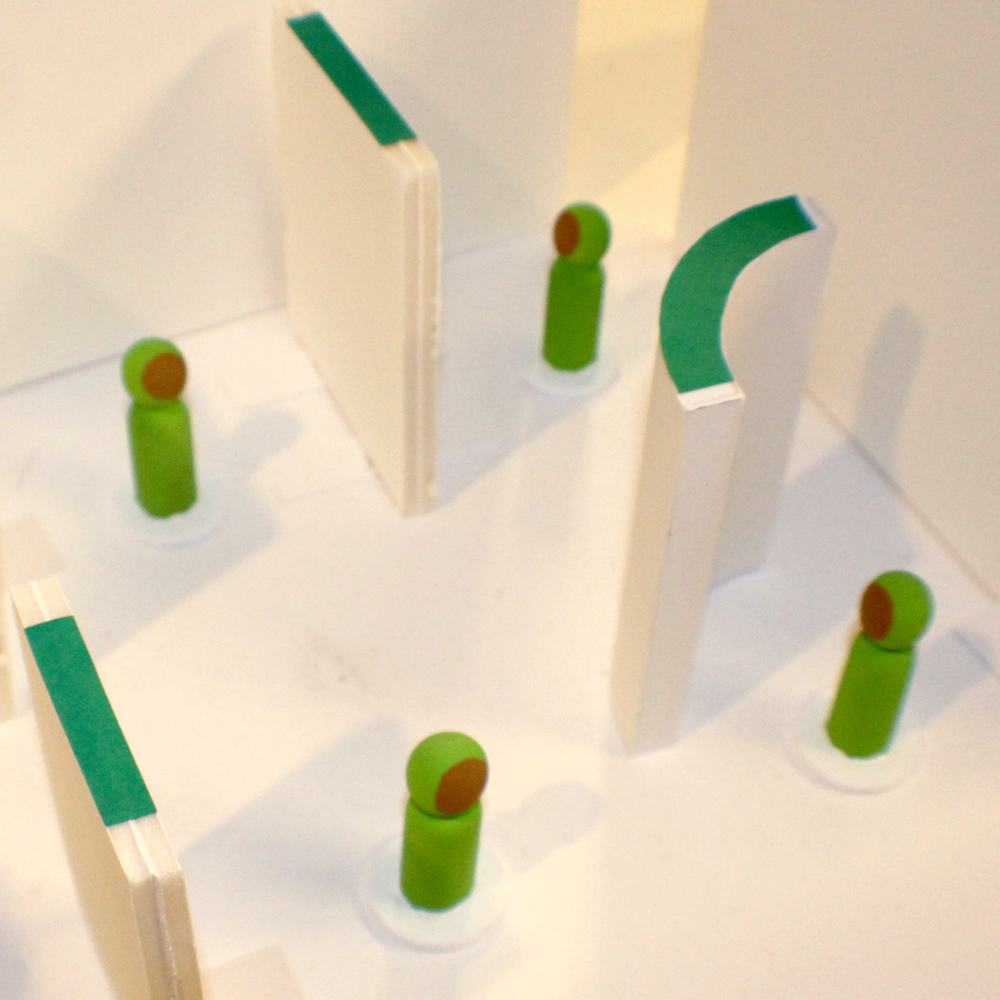
\includegraphics{photos/peeps1_crop.jpg}}
%\resizebox{!}{\picheight}{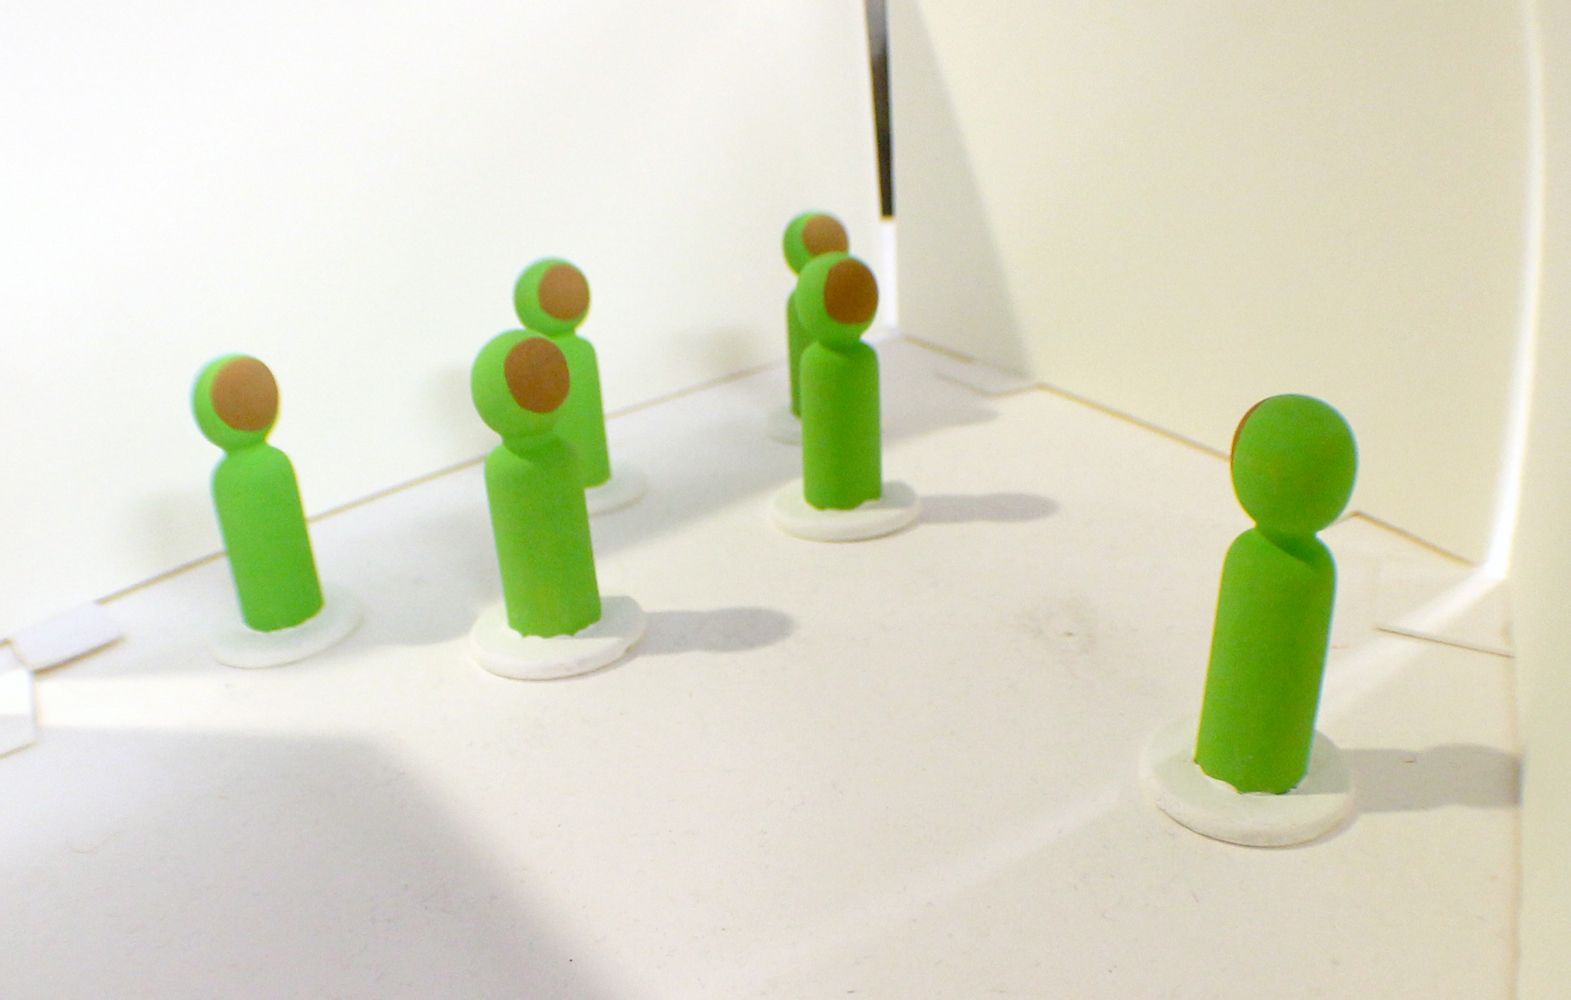
\includegraphics{photos/peeps2_crop.jpg}}
%\resizebox{!}{\picheight}{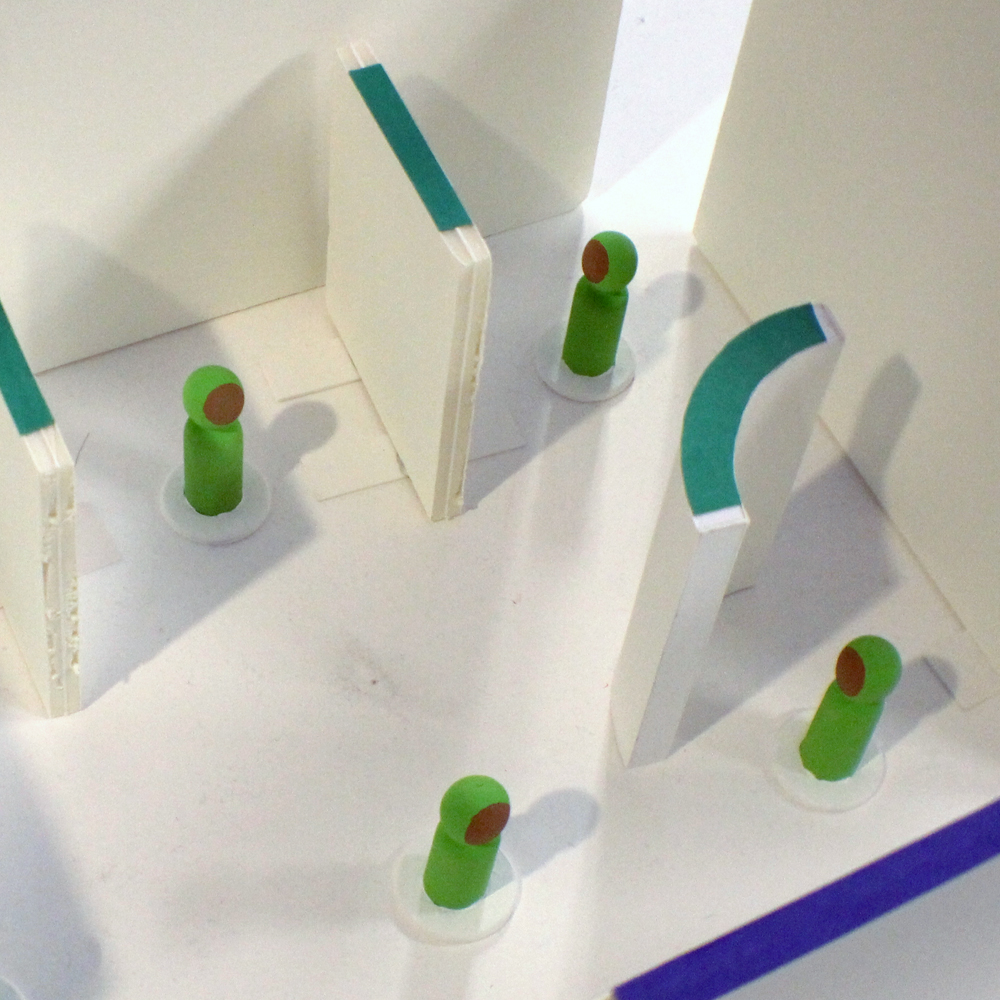
\includegraphics{photos/peeps4_crop.jpg}}
\resizebox{!}{\picheight}{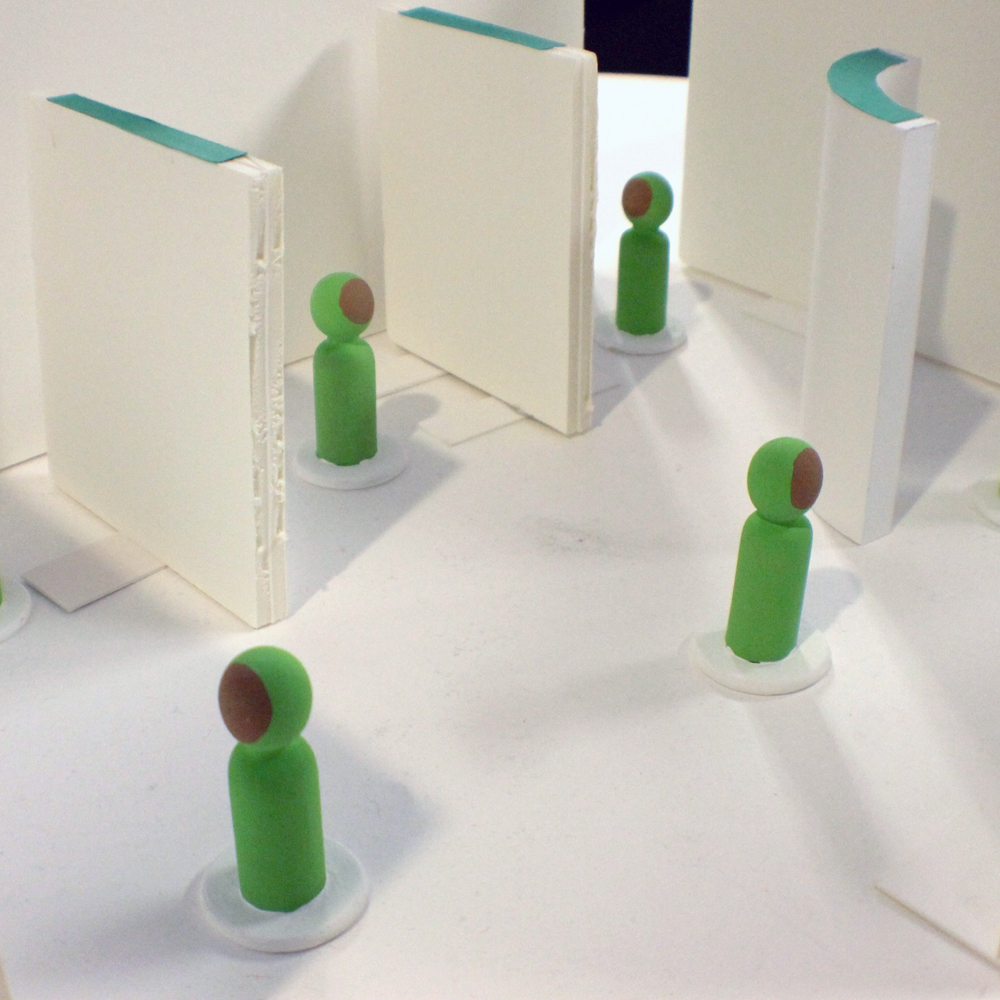
\includegraphics{photos/peeps5_crop.jpg}}%
%\resizebox{\picheight}{!}{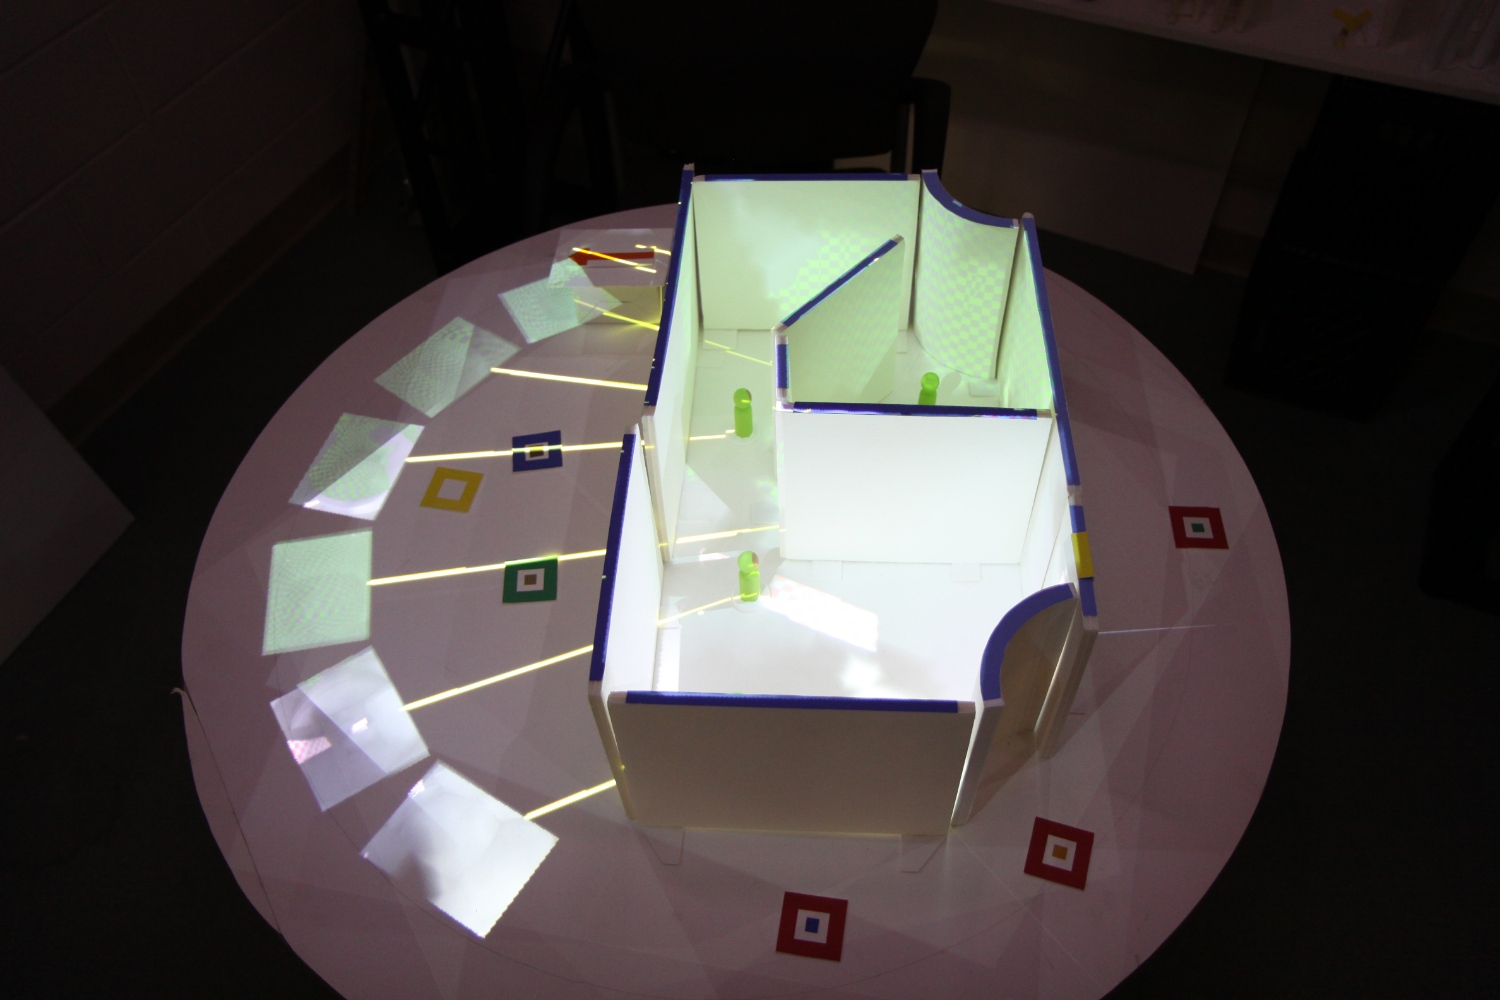
\includegraphics{photos/overhead_teaser.JPG}}
%\resizebox{\picheight}{!}{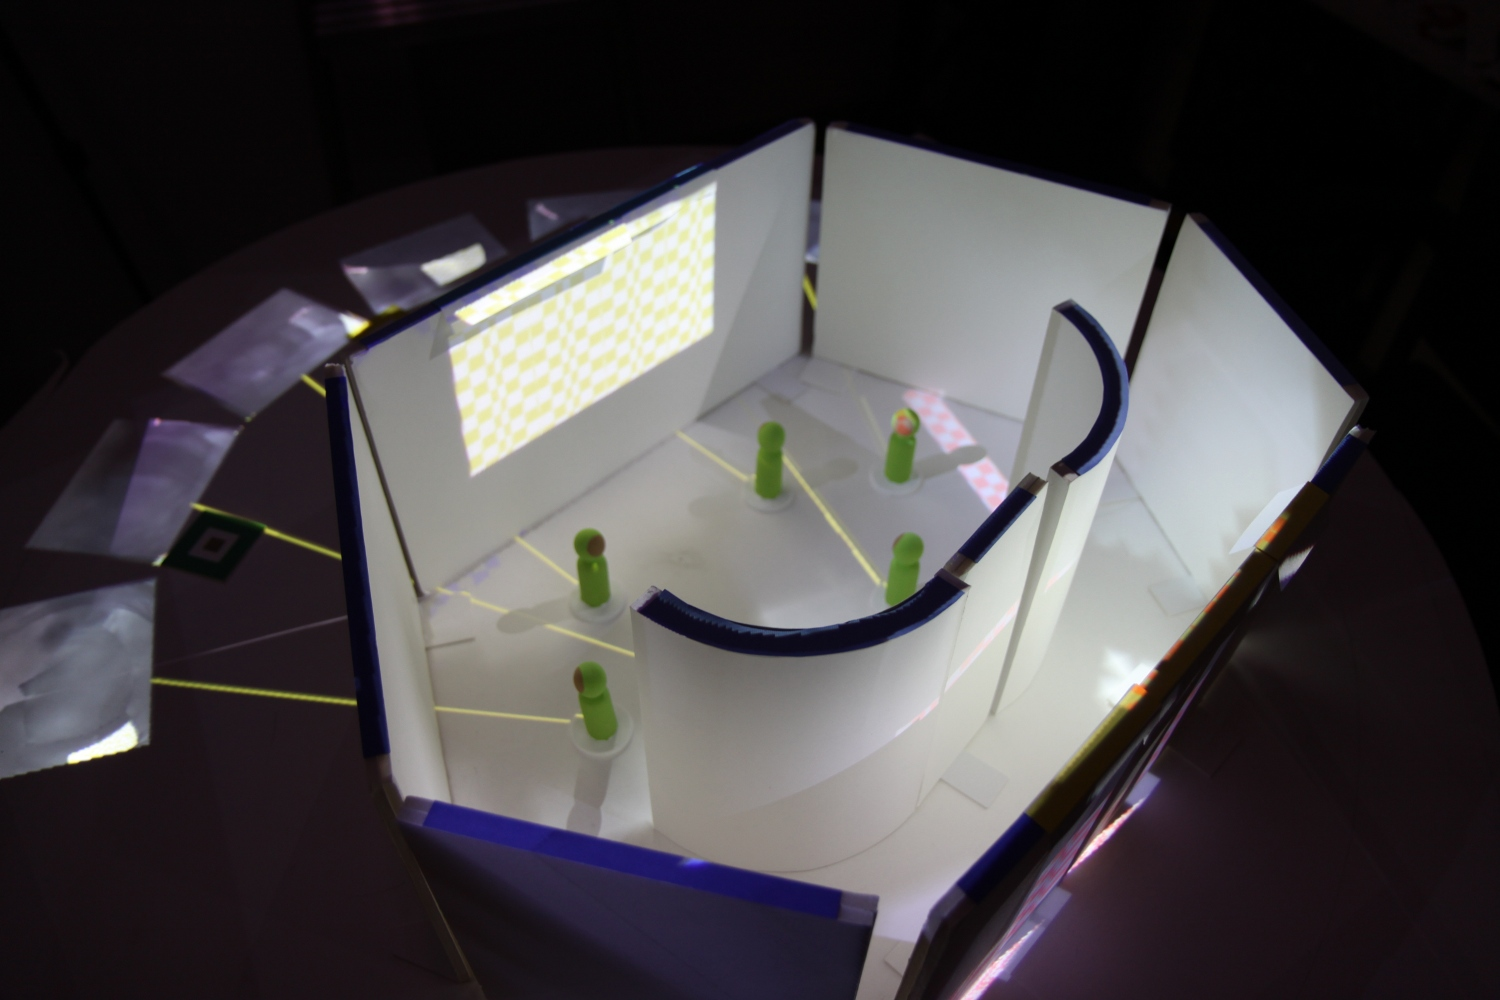
\includegraphics{photos/overhead_teaser2.JPG}}
\hfill%
\vspace{-2.49in}%
\resizebox{\picheightb}{!}{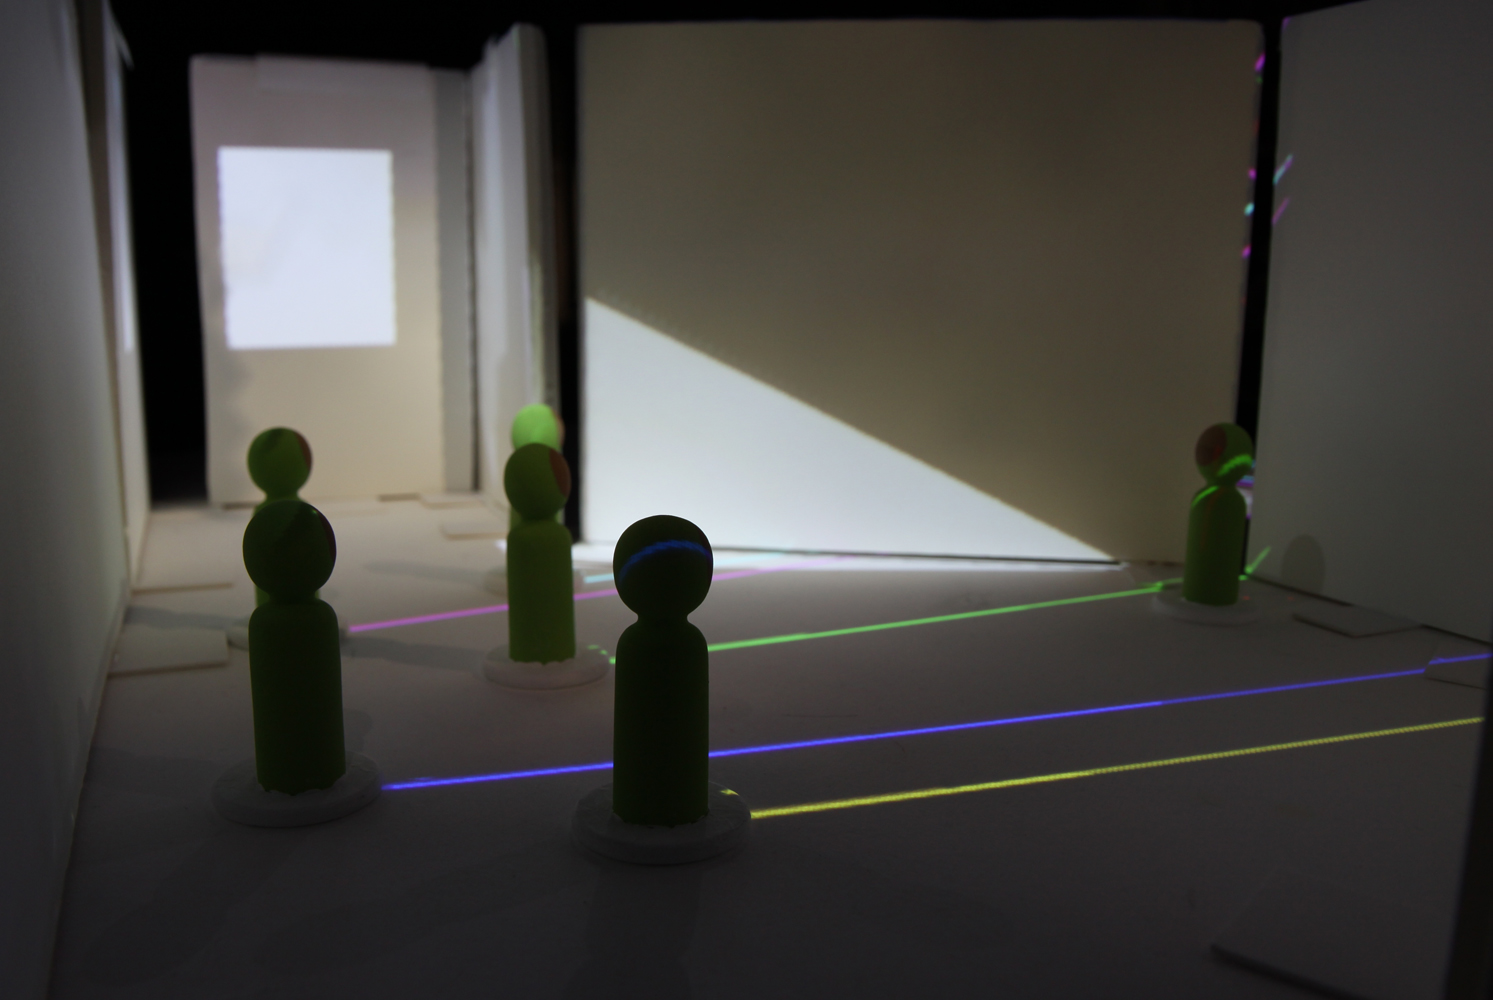
\includegraphics{photos/classroom_closeup.jpg}}\\
%\resizebox{\picheightb}{!}{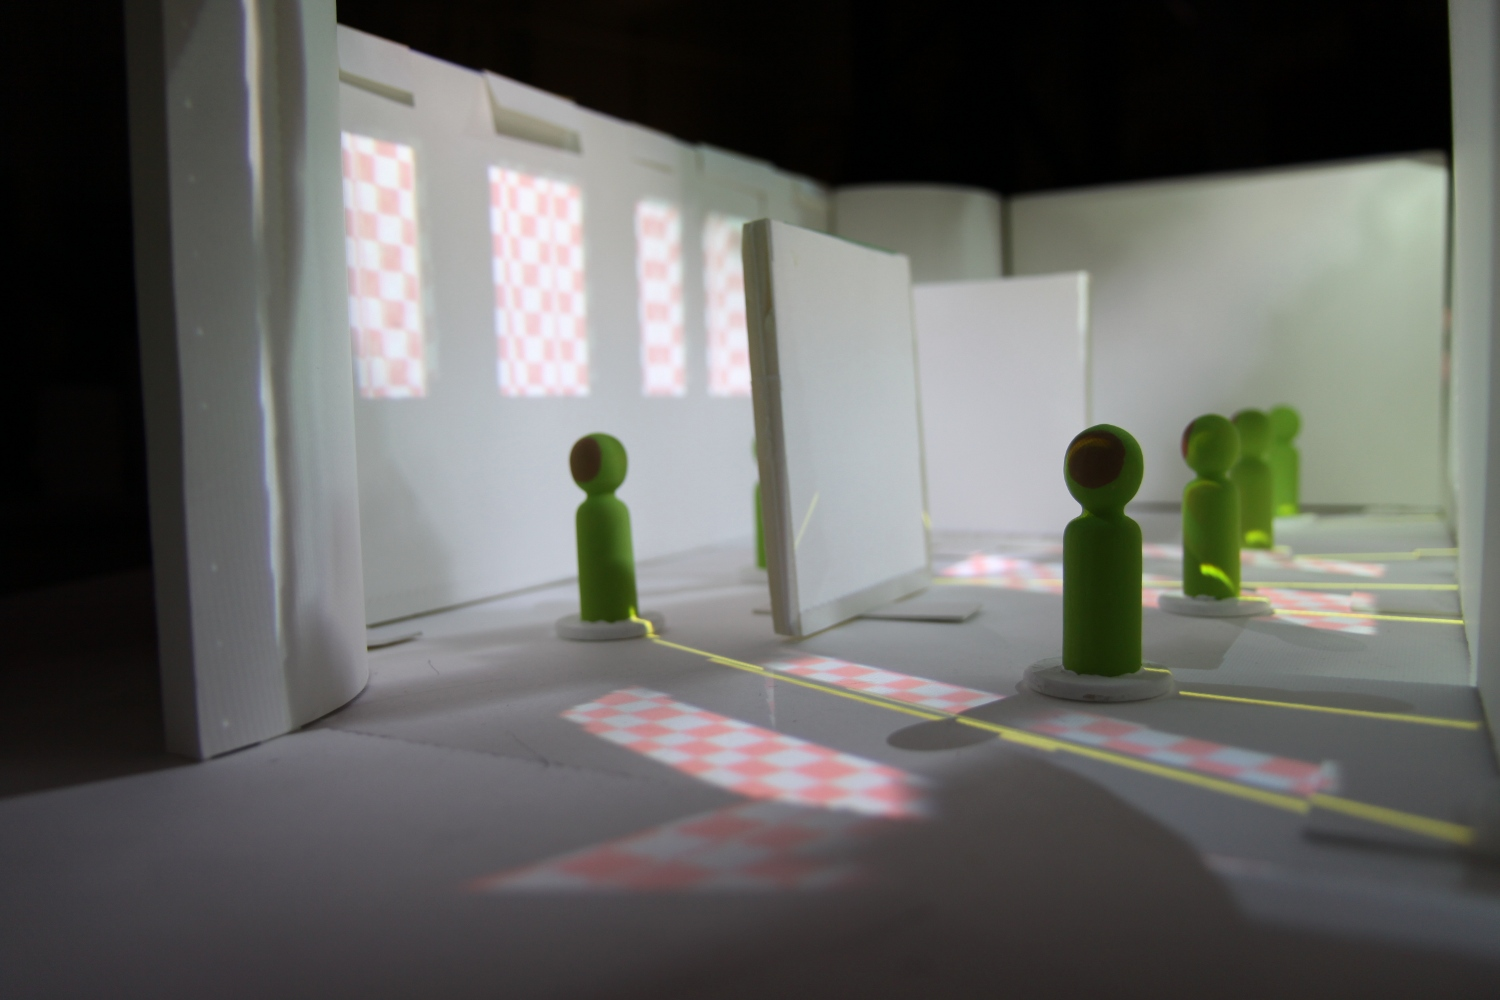
\includegraphics{photos/peeps_teaser.JPG}}\\
\hspace*{1in} \hfill 
\resizebox{\picheightb}{!}{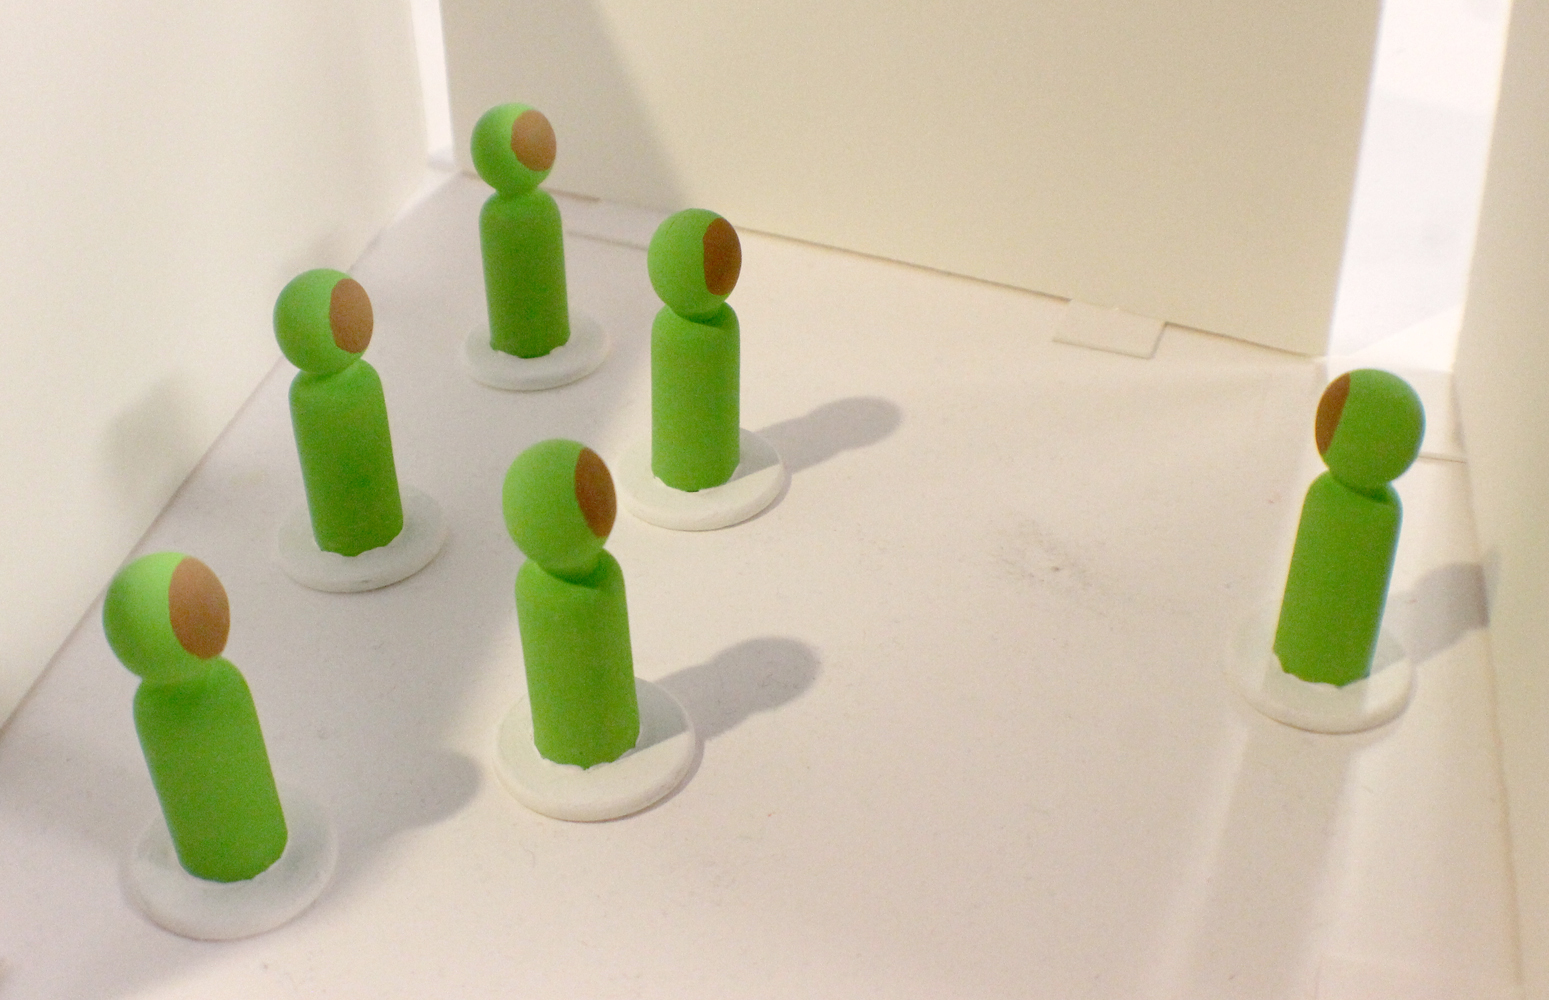
\includegraphics{photos/peeps3_crop.jpg}}\\
%\resizebox{\picheight}{!}{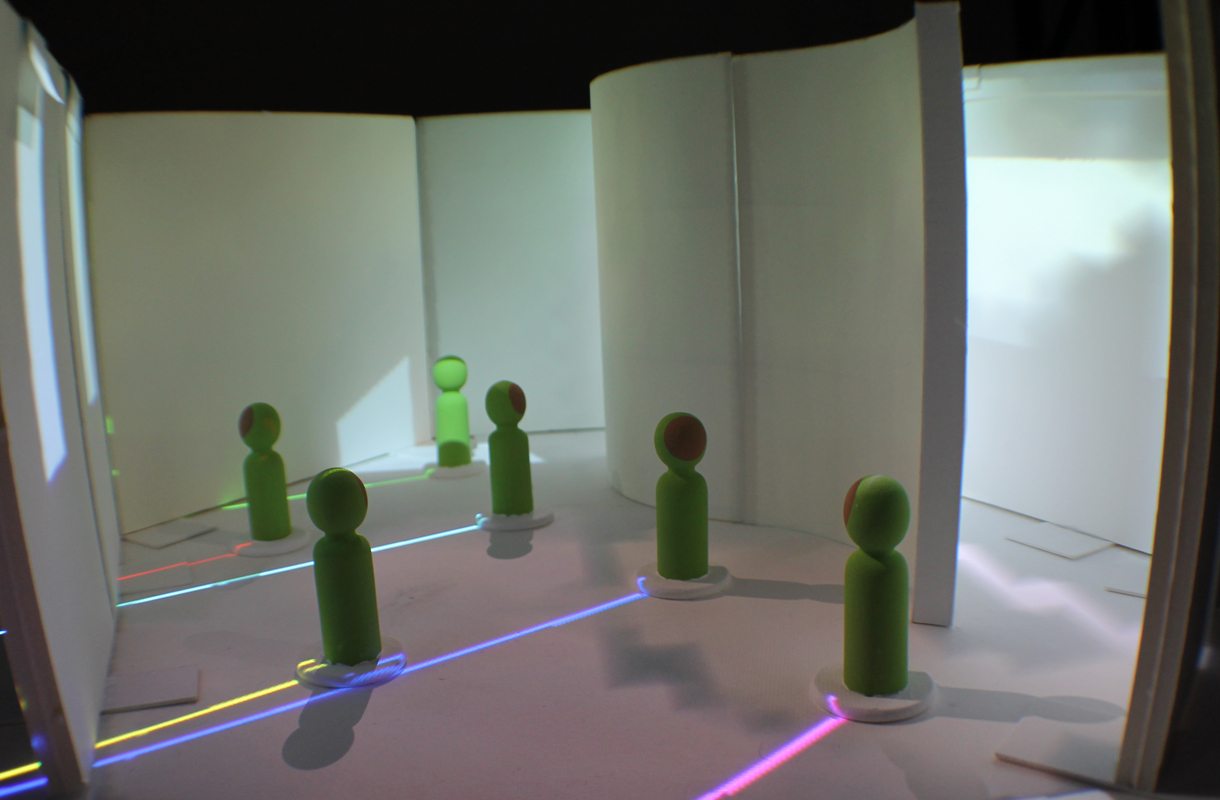
\includegraphics{photos/museum_fisheye.jpg}}

\vspace{1.15in}
%\vspace{-0.1in}
\caption{We provide new avatar tokens to specify the sample location
  and orientation of occupants in the space.  The ``face'' of each
  token is detected with the overhead camera.
%locations of
%  interest. 
The avatar tokens allow the designer to sketch the proposed
functionality of the space.  The examples above show how workers are
be oriented in a cubicle office environment and how a teacher and
students interact in a classroom.
%This provides the designer with
%users potential
%perspective view s of occupants in
%  the space.  
%Each avatar Both the position and the orientation of the token are
%  considered when providing the specified perspectives.
}
\vspace{-0.15in}
\label{FIGURE:teaser}
\end{figure*}

%%%%%%%%% BODY TEXT
\section{Introduction}

%\subsection{Tabletop system}

%We have extended a
%For our system 
%we use a Tangible User Interface, TUI, for

%For our system we use a Tangible User Interface, TUI, for
%architectural daylighting design.  The system allows sketching an
%architectural model with physical primitives (see Figure
%\ref{FIGURE:teaser}).  In order to create a complete model, a user
%places wall primitives, window primitives and a north arrow on the
%table.  In addition primitives to specify wall color, ceiling color,
%floor color and glare sensors are available.

\vspace{-0.05in}
We have developed a Tangible User Interface for visualization of
customized architectural daylighting simulations ~\cite{ShengYYC09, sheng_TVCG}. 
The user physically
constructs a small scale architectural model with physical walls
primitives shown in Figure~\ref{FIGURE:teaser}, adding tokens to mark
windows, specify surface materials, and indicate the surrounding
environment (north orientation).
%In order to create a complete model, a user
%places wall primitives, window primitives and a north arrow on the
%table.  
%
Additionally, small avatar tokens are placed within the model to
locate the typical position and usage of the space and measure the
directional illumination within the simulated volume.

%In addition primitives to specify
%wall color, ceiling color, floor color and glare sensors are
%available.

For each simulation, a single calibrated overhead camera captures the
scene.  Normally to capture 3D geometry at least two calibrated
cameras are required.  By having a single camera directly above the
table and indicating a few fixed wall heights with differently colored
top edges we are able to infer the full 3D geometry of the model.
Once the 3D geometry has been captured, a closed 3D mesh is generated
using the algorithm described in Cutler and Nasman~\cite{aag201015}.


Natural lighting from both the sun and the sky hemisphere is
calculated for the mesh for a specified time and day and geographic
location.  We use a variation of 
%
``Hardware-Accelerated Global Illumination by Image Space Photon Mapping"
%
%
\cite{mcguire09imagespace} to render an image of the virtual lighting
falling on each planar or curved surface in the physical model.
%
%Rendering daylighting requires another level of complexity than
%rendering with point light sources.  
%
Our simulation separates the direct light computation from the global
indirect illumination which is computed using photon mapping.  There
are four standard sky types that are used for daylighting simulation:
clear sky, intermediate sky, turbid sky and overcast sky
\cite{international1994spatial,perez1990modeling}.  Each of these
models requires the illuminance value for the zenith
\cite{Karayel1984283} and measurements of the illuminance for the
ground plane.  For the renderings in the paper, we use the CIE clear
sky model.

Our multi-projector system is run in a master slave configuration.
The master sends the surface images to each process on the slave
computers.  Each process renders the geometry of the scene with the
image textures overlaid on each wall.  A common projection blending
algorithm 
%
~\cite{Raskar:2001:SLA}
%\fbox {cite A RASKAR PAPER.... shader lamps?} 
takes into account
%
the visibility and occlusions of the surfaces for each projectors and
produce a smooth final illumination result on the physical model.
The technique of projecting information onto a physical model is known as
Spatially Augmented Reality (SAR).

The system allows users to make physical sketches with foam core walls
in three heights: 5", 8", and 10".  Window markers are available in
two colors to create taller and shorter windows.  Once a design has
been completed, the user can request a time and date for simulation.
In a normal interactive workflow, the user will request several times,
make modifications to the room, request additional simulations, and
iterate until they are satisfied with the design.  We conducted a user
study of the initial system and found that users had difficulty
identifying which areas of the room were too bright, too dark, or had
glare problems.  Users also expressed interest in having options for
more complicated window materials and lighting controls.  For this
reason we updated the physical controls of the system, the
visualization modes, and window materials.




%\subsection{A Tangible Interface Integrated with Augmented Reality}
%\fbox{Is this where we put this?}

Our system leverages a Tangible User Interface (TUI) for interactive
design, which allows quick sketching of architectural spaces.  This is
beneficial and convenient even for users who are familiar with
standard design software tools, because the TUI provides an simpler
interface to create initial rough draft models.  A simple model can be
created in as little as 30 seconds in our interface.  In order to
create a similar model in a CAD drafting tool it would take minutes
instead of seconds.  Importantly, it is simple to make edits to the
model in response to the simulation results.  Our tool provides tokens
to control the most important aspects of model for daylighting: window
placement and proportions, surface materials, and building
orientation.


%\fbox{Need to describe specific benefits of TUI. }
%\fbox{Discuss caves, Oculus rift, other options (none provide all of the benefits of our system}
%
In additional to SAR there are several
other options for displaying a 3D perspective of a real or virtual
environments, including head
  mounted displays , CAVEs, etc.  However, the other options do not offer the same
ease of design, intuitive omni-directional display, 
 face-to-face engagement with other users,
and simultaneous visualizations for
 multiple virtual viewpoints.
%
By combining these factors, we provide a powerful interface that allows
the design process and lighting evaluation to happen simultaneously
without the need to switch between various tools.
%\fbox{paragraph could be revised more}

\subsection {Our Contributions}

\noindent
The contributions we present in this paper are:
\vspace{-0.1in}

\begin{itemize}
\item An effective, quantitative false color visualization
  for use in analyzing areas of over- and under-illumination. \vspace{-0.1in}
\item Provide avatar tokens for users to place within the a
  physical small-scale model of a room to measure potential
  \emph{glare} problems (negative impacts on vision due to the
  presence of bright light in a person's view). \vspace{-0.1in}
\item Provide the option for users to put complicated window geometry
  into their model while providing them with both a high detail
  rendering and accurate lighting information.
\end{itemize}


\section{Related Work}

\paragraph{Tangible User Interfaces}
%
An early TUI developed by Ishii and Ullmer~\cite{Ishii97tangiblebits}
allowed users to manipulate digital information by controlling their
system with physical icons.  Jacob et al. extended the TUI
by projecting information on movable physical
objects~\cite{Jacob01atangible}.  The ``bricks'' system was the first
interface to allow multiple physical controls in a TUI system to be
used together to expand information shown~\cite{223964}. 
%
% \fbox{weird
%  mix of using the authors names and just mentioning the name of the
%  system, go with one or the other... } 
%
%Using names of the system when 3 words or less are used because ofthen
% the description helps.  If theres not a name for the system and the 
% paper name is long winded, just writing author names
The ``JUMP" tool continued to improve controls for a TUI by using a
variety of tokens in a projector-camera system to allow users to
switch between multiple architectural documents to rectify
them~\cite{1268540}.  
%
Inspired by these systems, we allow users to switch between layers of
data: a daylighting rendering and a false color visualization mode of
the same model. 
%
The ``URban Planning" system provided an interface that enabled users to
see how buildings would cast shadows on each
other\cite{Underkoffler:1999:ULW:302979.303114}.  Our system also
displays daylighting in architecture but focuses analysis on 
%designed
%to simulate 
propagation and distribution of light in the interior spaces.
%\fbox{more analysis}




\vspace{-0.1in}
\paragraph{Projector Camera Interfaces}
%
%Need to tie these in better?
%
%
%Projector Camera systems have been used in a variety of ways to
%communicate information. Mitsugami used multiple moving projectors
%together to produce a single image\cite{MitsugamiUK07}.  While we are
%using a system with six projectors, dynamic alignment of projectors is
%unnecessary because our projectors' positions are static.  Barnum
%created a projector camera system which used falling water drops as a
%projection surface\cite{Barnum09aprojector-camera}.
%
Projector-camera systems are well suited to convey 3D information.
Amano printed a normal map on paper and then used a
projector camera system to project an image of the model with a
light's location changing~\cite{DBLP:conf/cvpr/Amano12}.  While their
system only projects on a single 2D surface, our system projects simulation
data onto a 3D model. Gartska and
Peters used a Kinect to track a user's head position and
orientation~\cite{Garstka_Peters_2004}.  Based on this information, a
projection of a 3D image was changed so that it appeared the user
moved in relation to a 3D object.  Menk and Koch~\cite{menkandkoch}
projected a simulated 3D reflected surface onto a colorless 3D model while taking into
account ambient light.  We also simulate light in a virtual model and
project it onto a real surface but Menk and Koch were incorporating
the lighting from the actual environment on a real physical geometry whereas we are
running a full daylight simulation on a scale model of a space.



An early example projecting 
%\emph{Spatially Immersive} 
spatially immersive information on every day surfaces was The Office of the Future
\cite{Raskar:1998:OFU:280814.280861}.  This work was extended in
Shader Lamps\cite{Raskar:2001:SLA}.  Similarly to Raskar et al.
\cite{Raskar:2001:SLA}, Sheng et al.\cite{ShengYYC09, sheng_TVCG}, and Yapo et al.
\cite{5543463}, our system projects information on neutrally colored
physical primitives to create a detailed rendering of a simulated
space.  Our physical primitives and rendering options provide unique
extensions to their work.




\begin{figure*}[t]

\begin{center}
\newcommand{\picheight}{2.325in}
\resizebox{!}{\picheight}{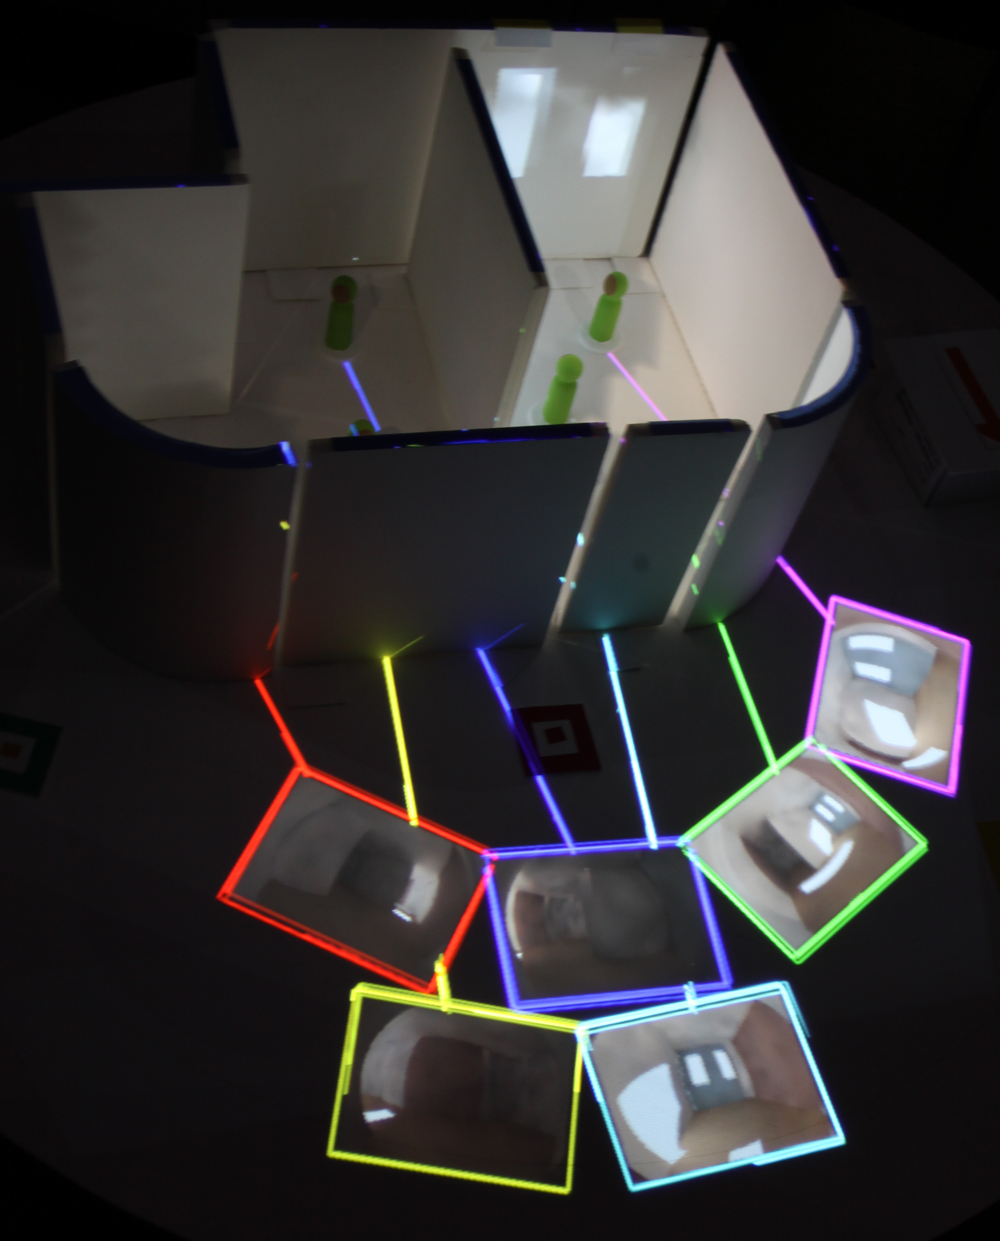
\includegraphics{photos/office_color.jpg}}
\resizebox{!}{\picheight}{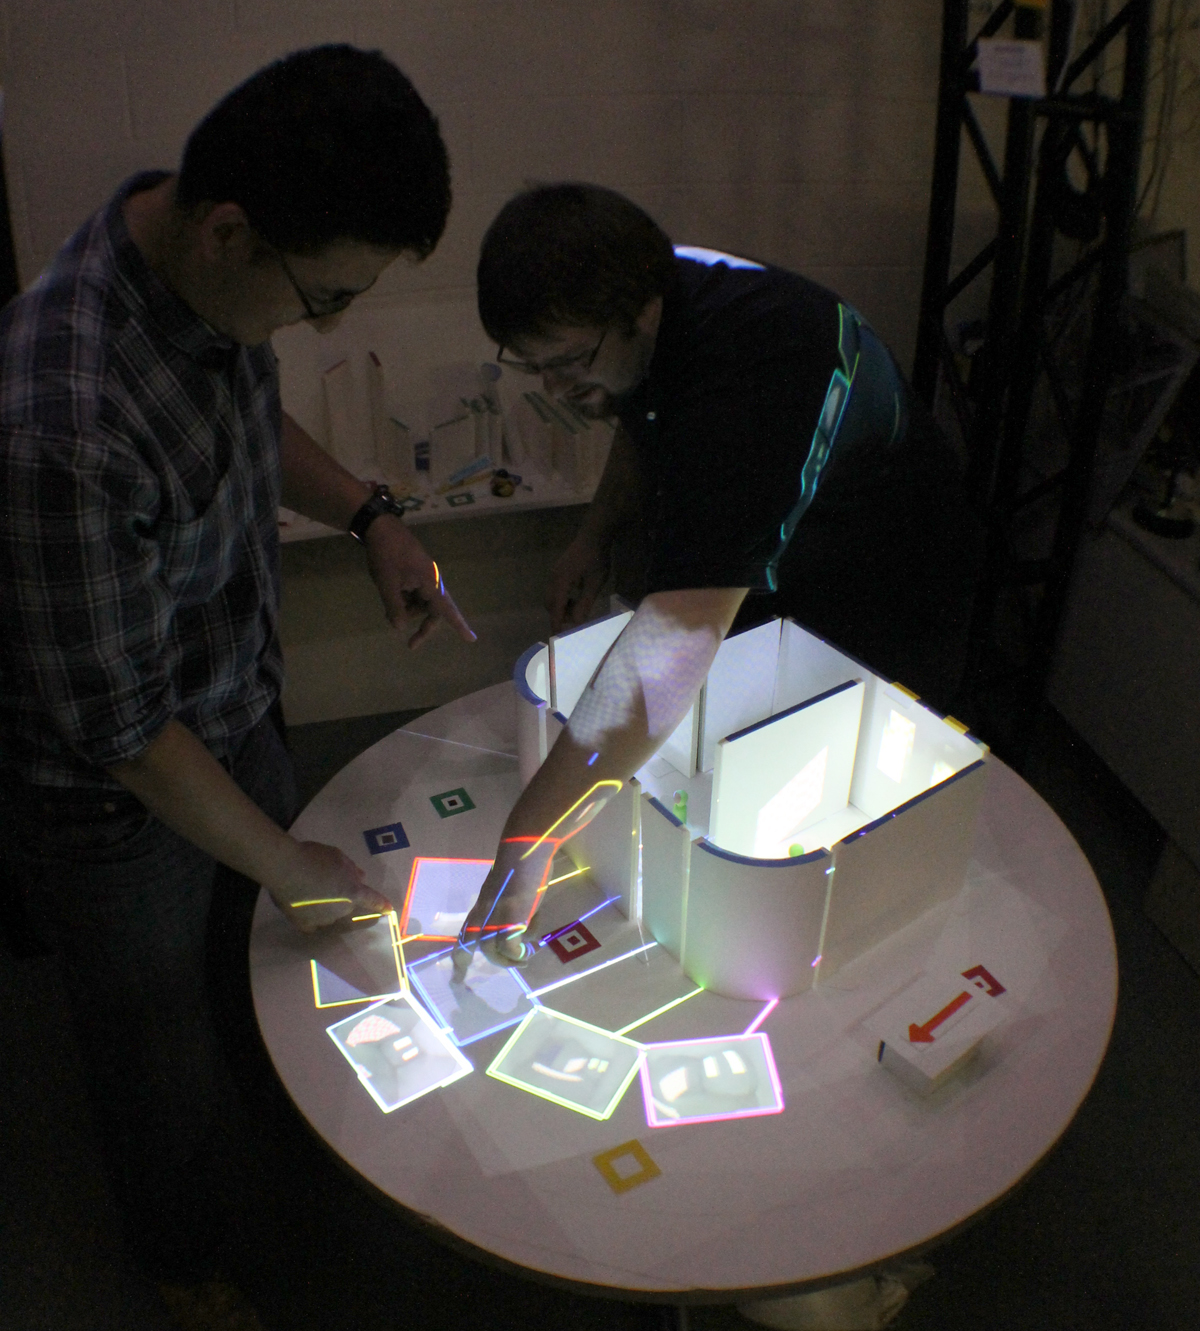
\includegraphics{photos/ian_matt_pointing.jpg}}
\resizebox{!}{\picheight}{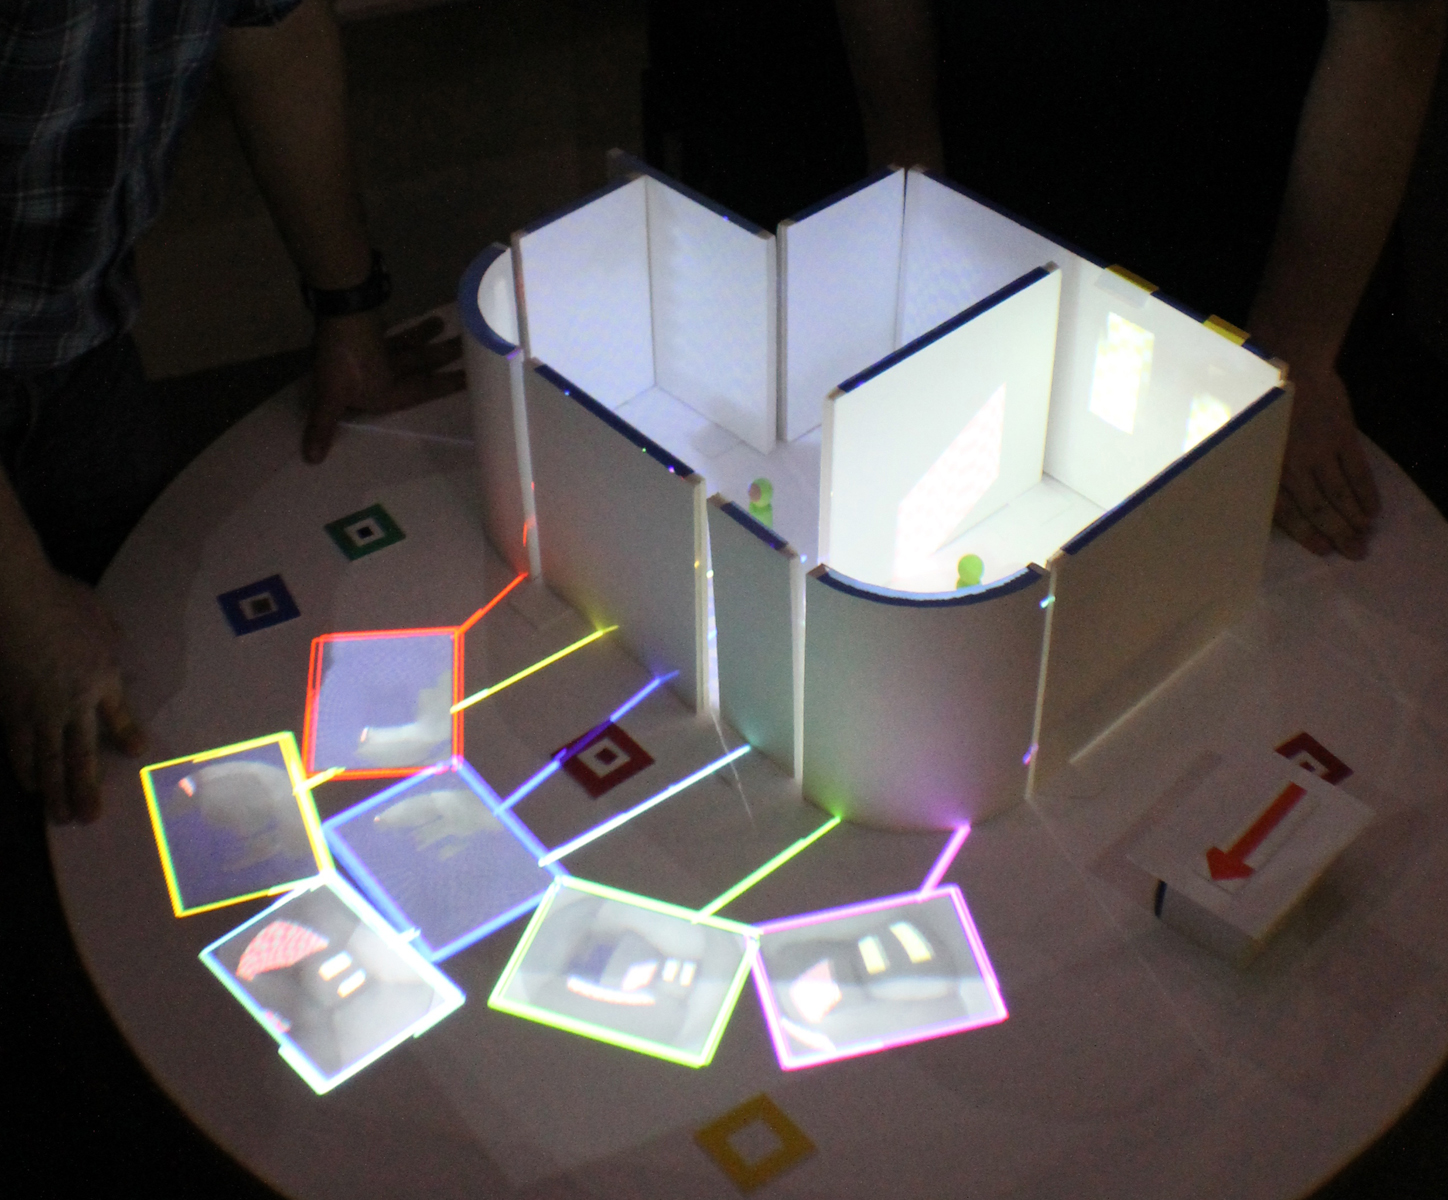
\includegraphics{photos/office_falsecolor.jpg}}
\end{center}
\vspace{-0.1in}
\caption{The most common difficulty for participants in our user study
  was in determining the significance of areas that were too bright or
  too dark.  Our false color rendering mode improves this visualization challenge.
%will help future user
%  discern where the problem areas are.  
Areas overlaid with a blue checkerboard are
  under-illuminated and the red checkerboard indicates an
  over-illuminated area.  The view point from each physical avatar are projected next to the model and also
  shown in Figure~\ref{FIGURE:fisheyes}.}
%\vspace{-0.15in}
\label{FIGURE:office_false_color}
\end{figure*}



\begin{figure*}[t]
\newcommand{\picwidth}{.955in}
%\resizebox{\picwidth}{!}{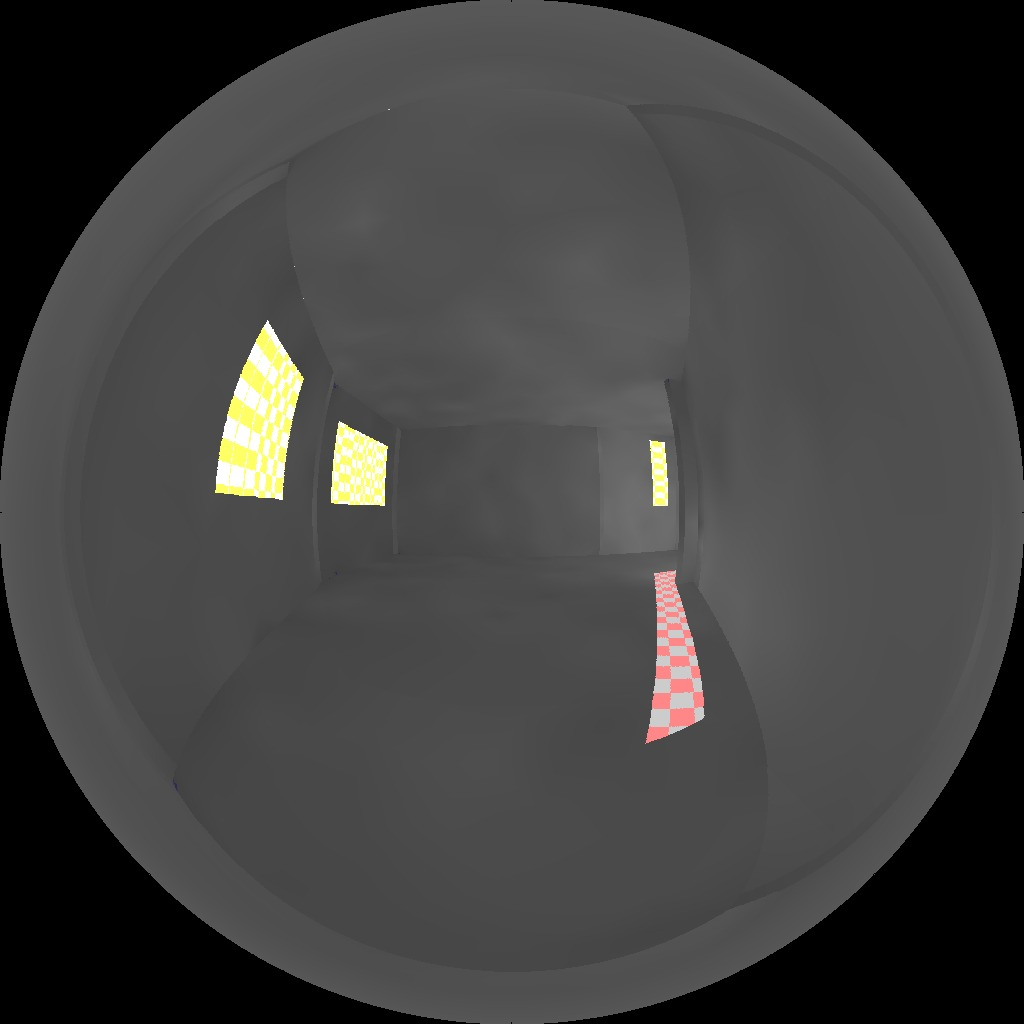
\includegraphics{wallfiles/classroom_12PM/surface_camera_VIEW_person0.jpg}}
%\resizebox{\picwidth}{!}{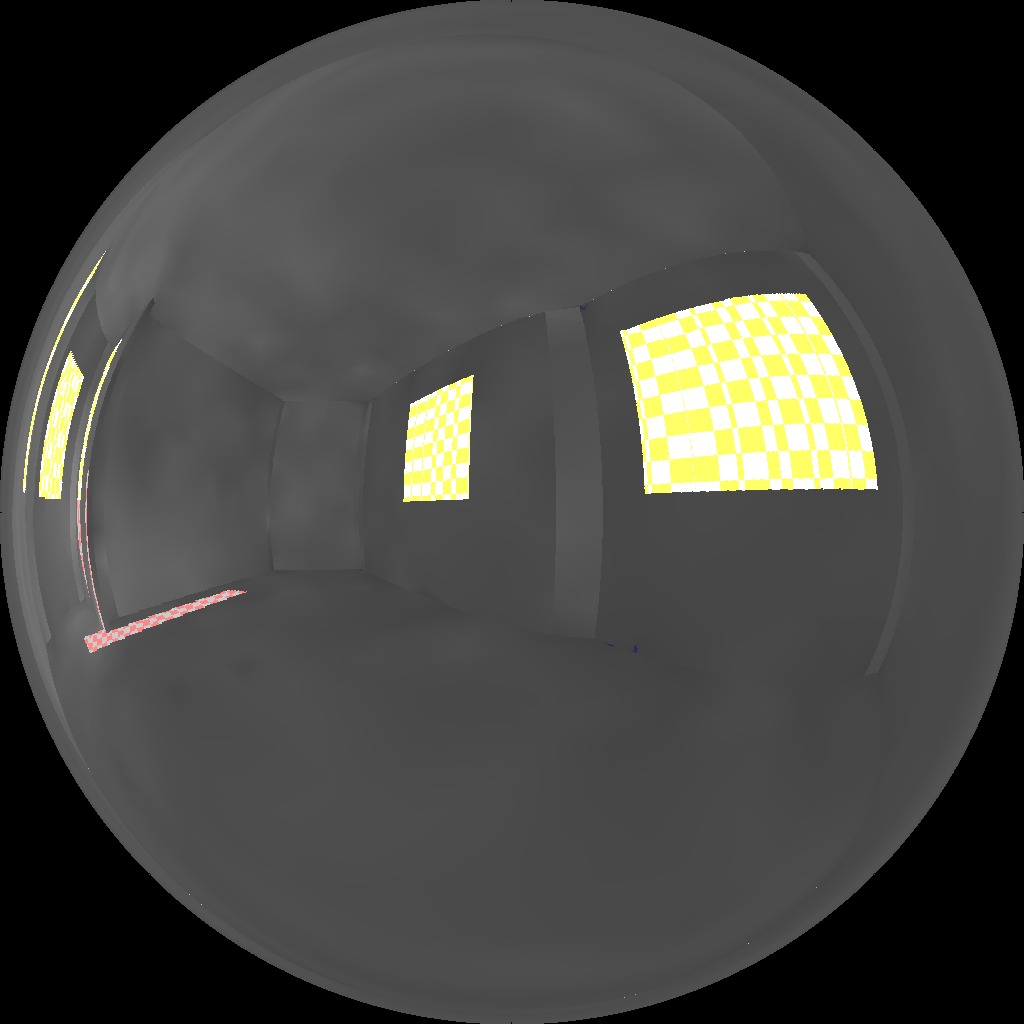
\includegraphics{wallfiles/classroom_12PM/surface_camera_VIEW_person1.jpg}}
%\resizebox{\picwidth}{!}{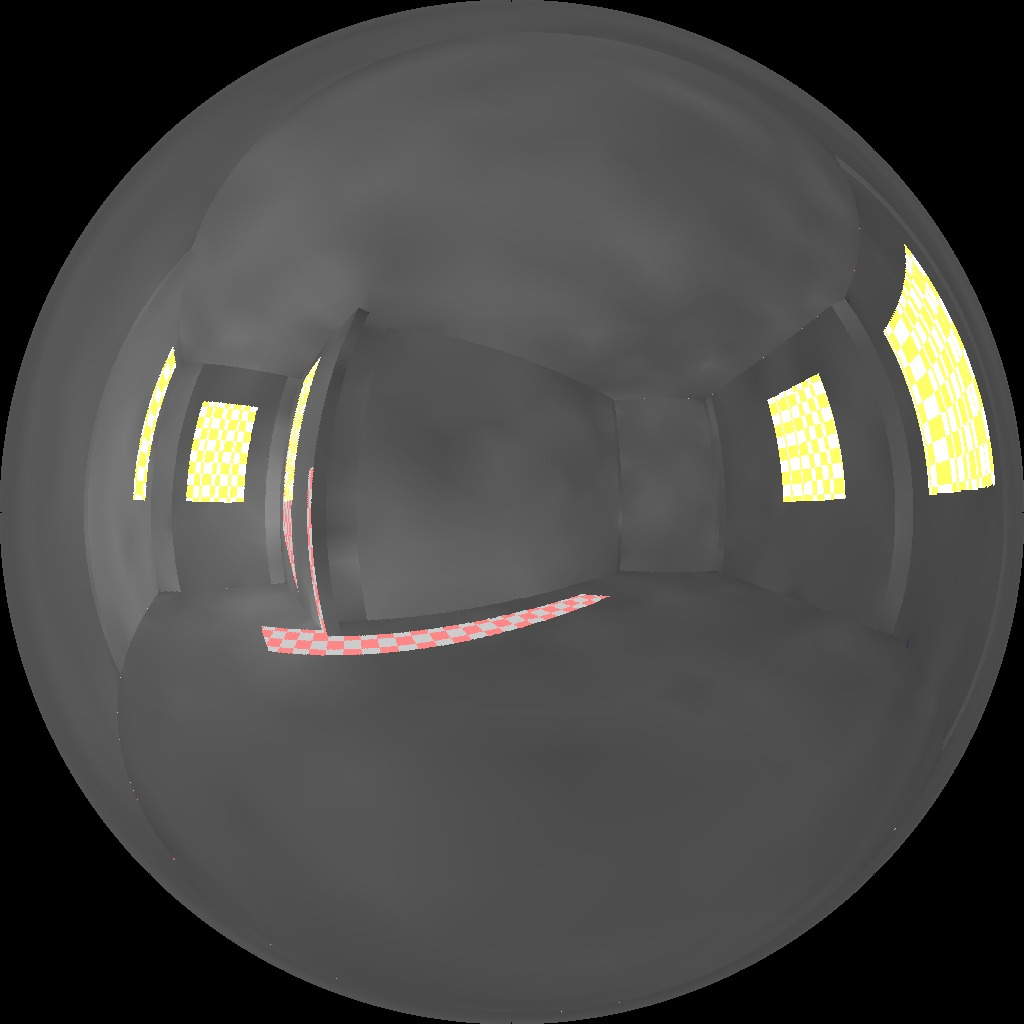
\includegraphics{wallfiles/classroom_12PM/surface_camera_VIEW_person2.jpg}}
%resizebox{\picwidth}{!}{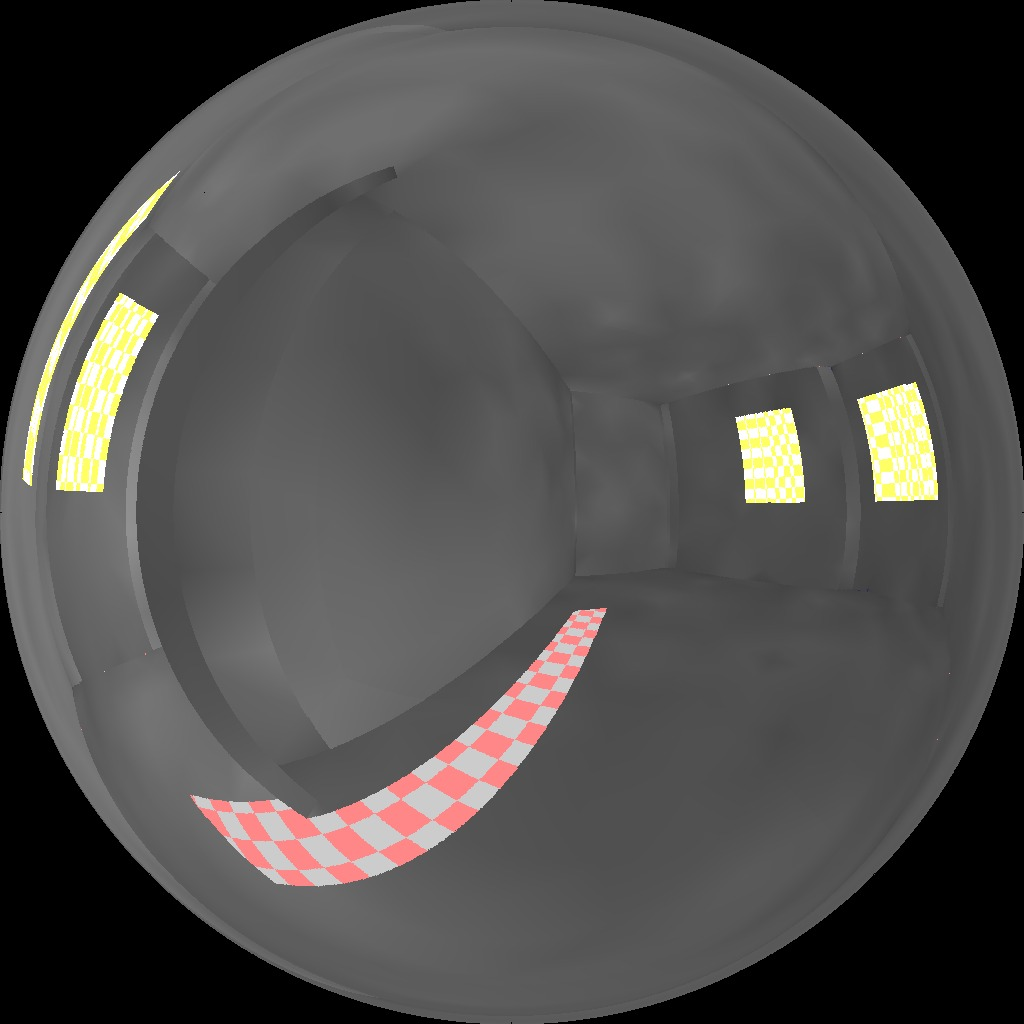
\includegraphics{wallfiles/classroom_12PM/surface_camera_VIEW_person3.jpg}}
%\resizebox{\picwidth}{!}{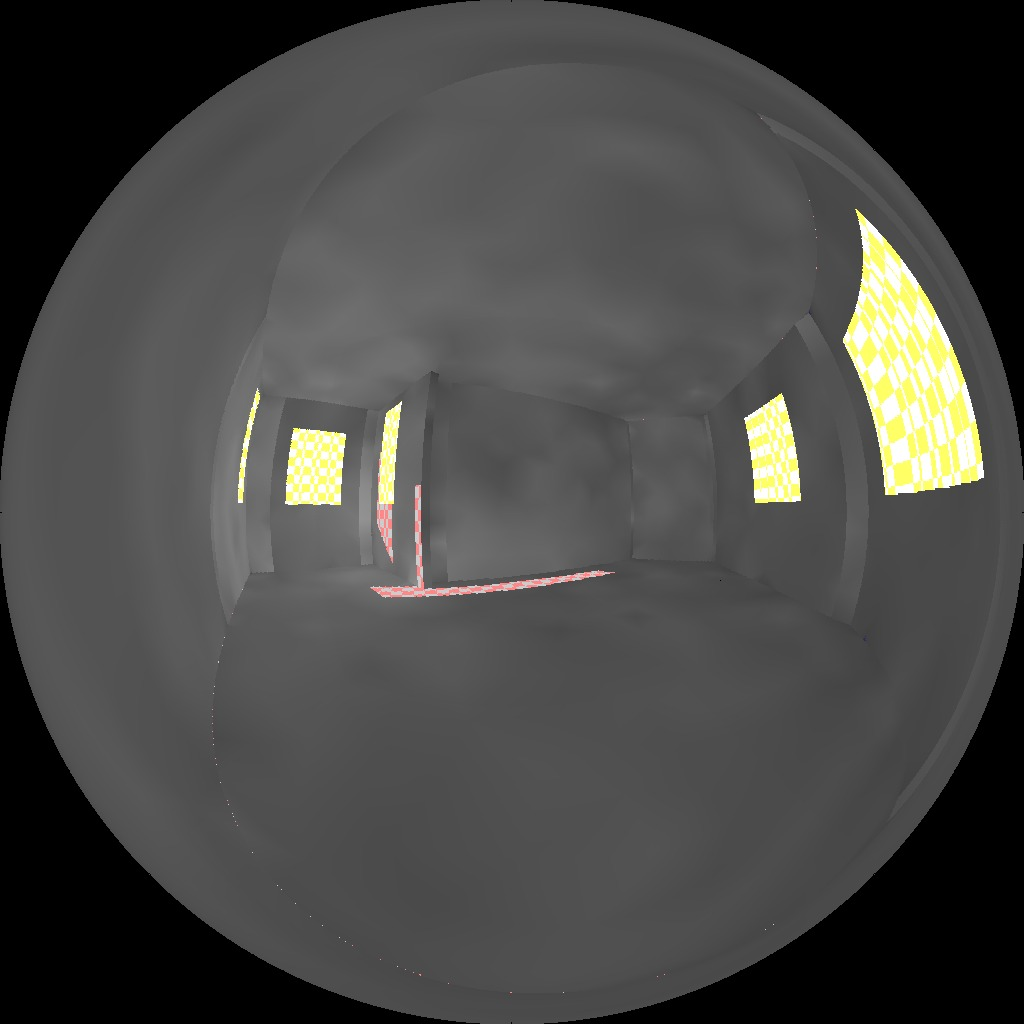
\includegraphics{wallfiles/classroom_12PM/surface_camera_VIEW_person4.jpg}}
%\resizebox{\picwidth}{!}{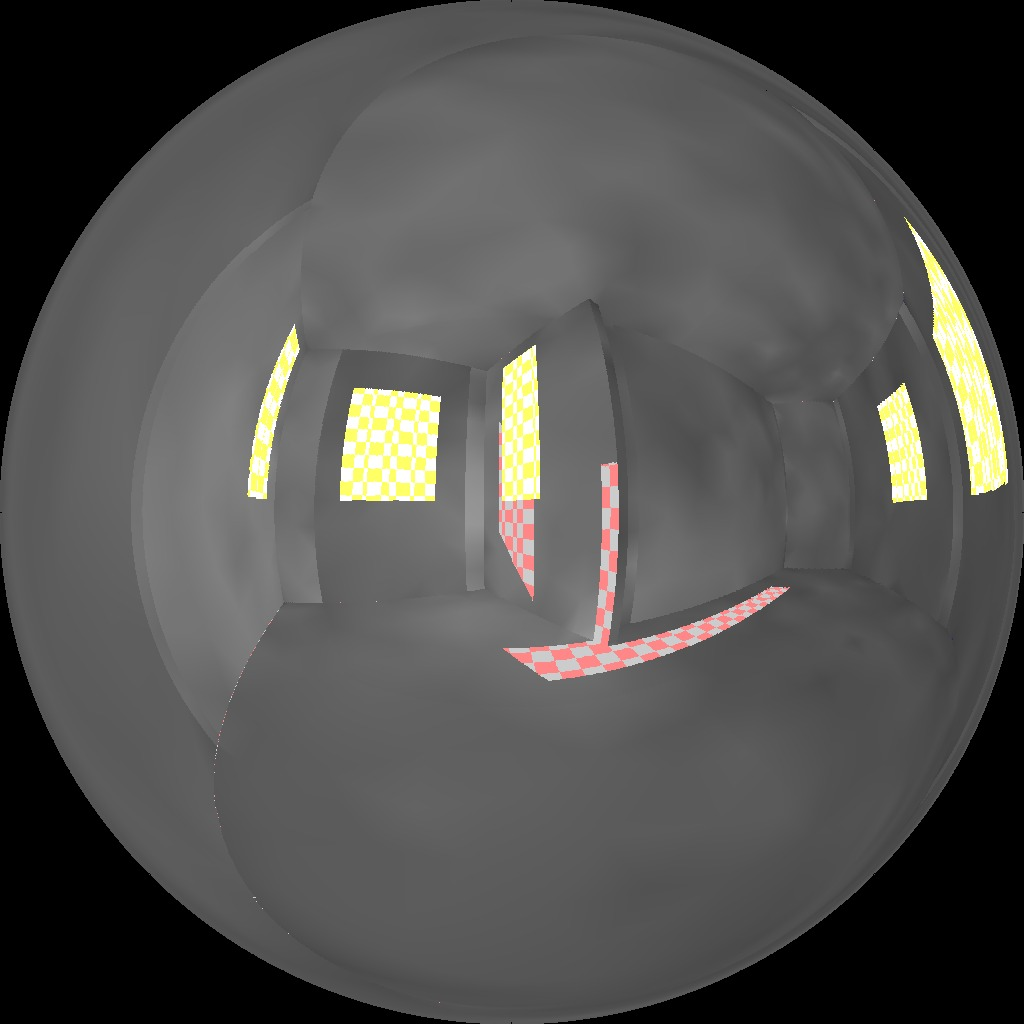
\includegraphics{wallfiles/classroom_12PM/surface_camera_VIEW_person5.jpg}}
%\\
%\resizebox{\picwidth}{!}{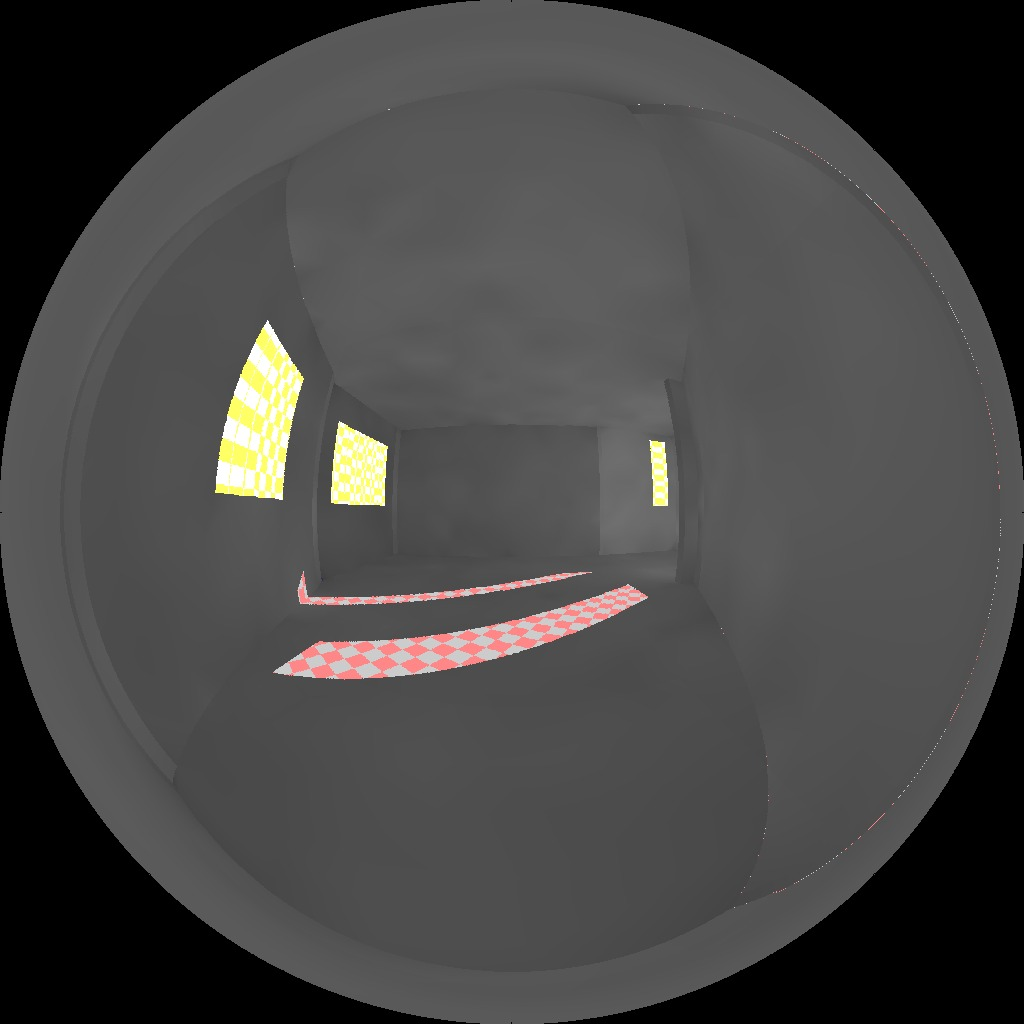
\includegraphics{wallfiles/classroom_2PM/surface_camera_VIEW_person0.jpg}}
%\resizebox{\picwidth}{!}{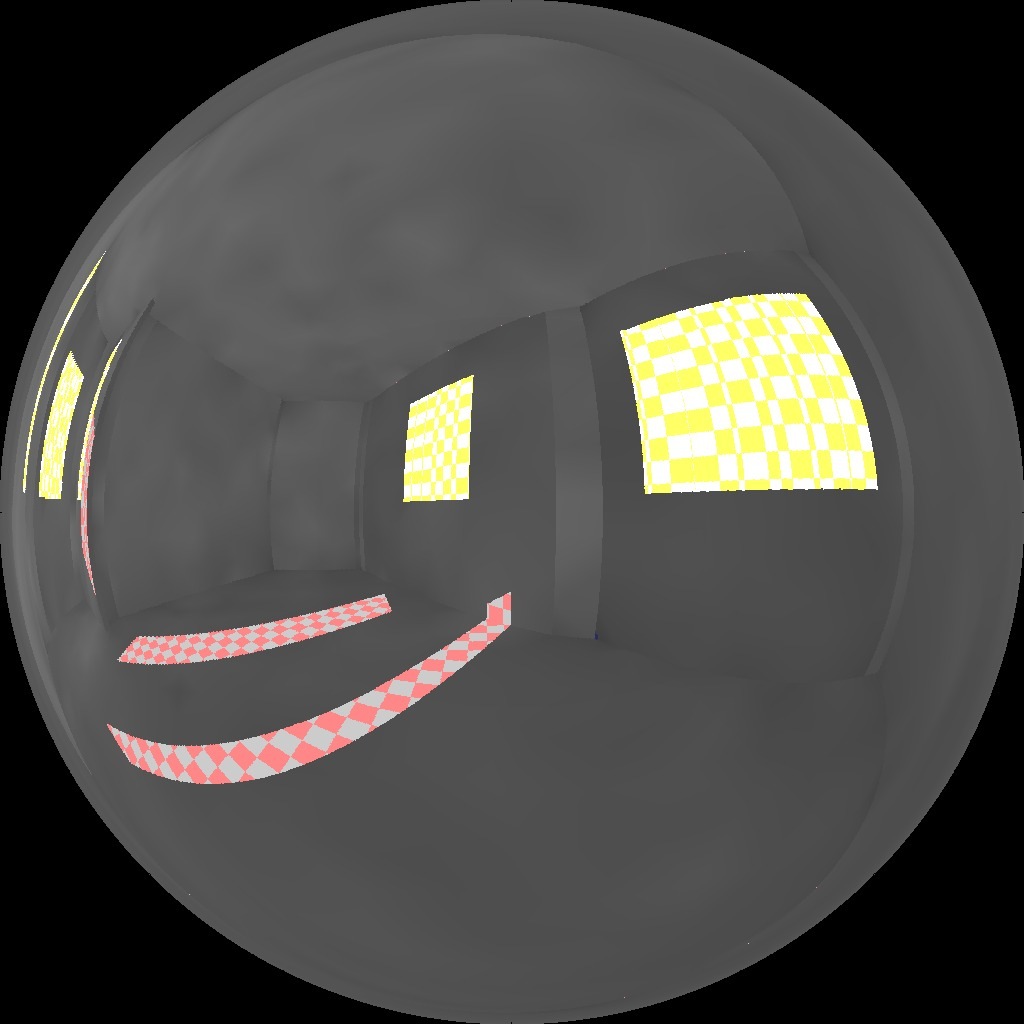
\includegraphics{wallfiles/classroom_2PM/surface_camera_VIEW_person1.jpg}}
%\resizebox{\picwidth}{!}{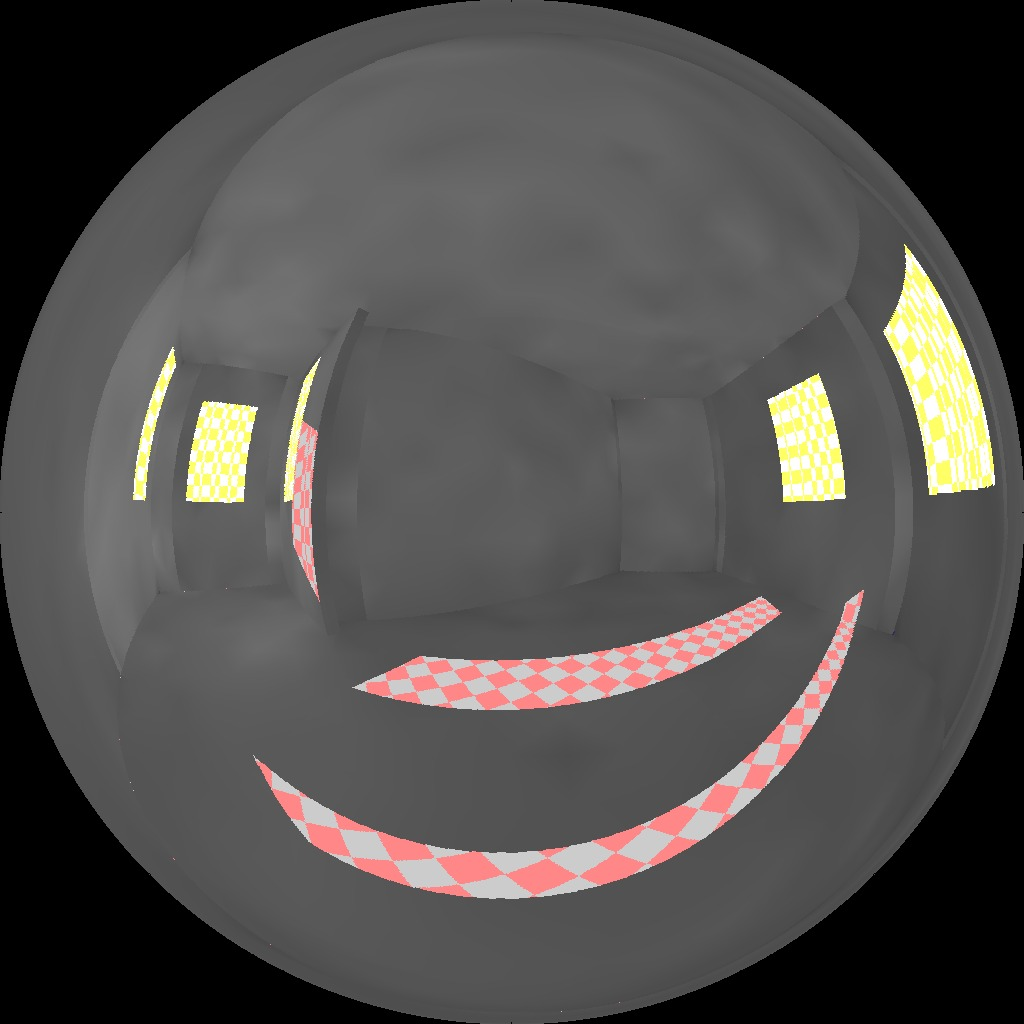
\includegraphics{wallfiles/classroom_2PM/surface_camera_VIEW_person2.jpg}}
%\resizebox{\picwidth}{!}{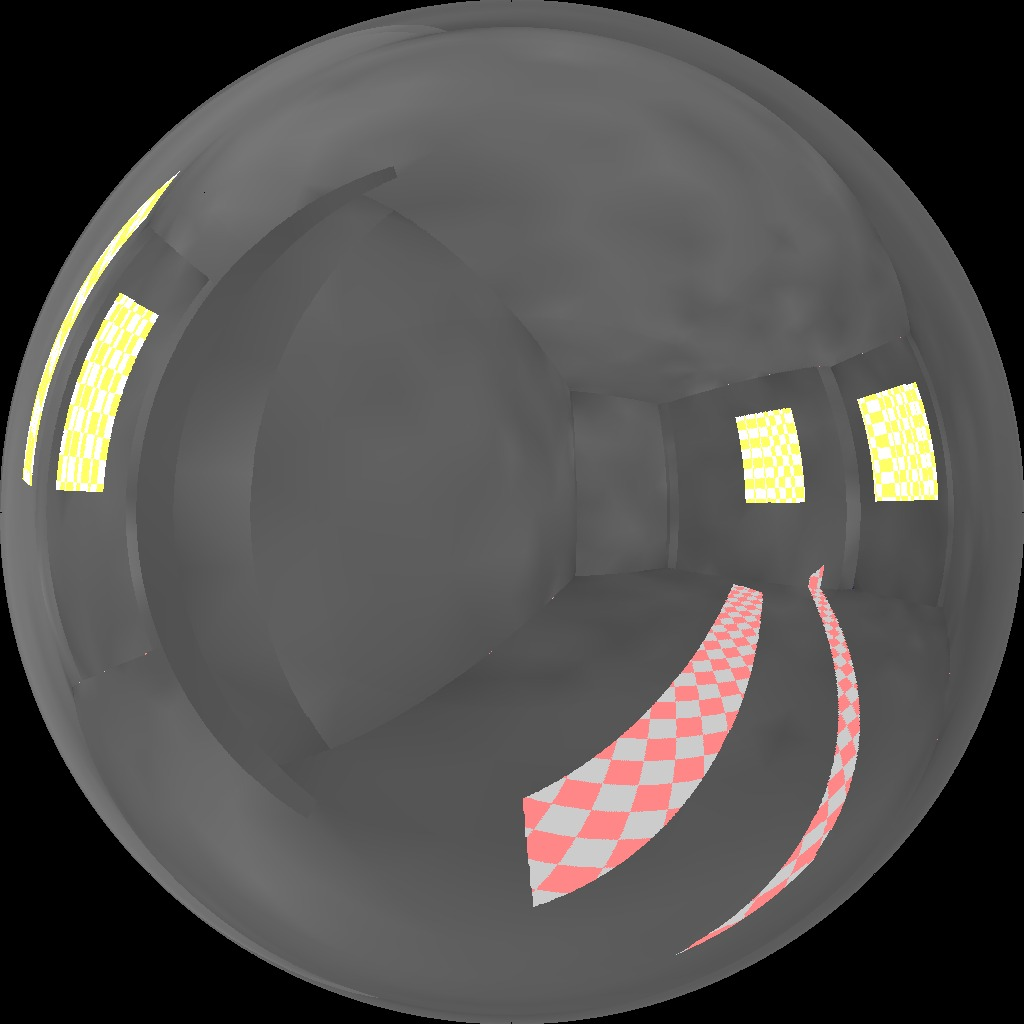
\includegraphics{wallfiles/classroom_2PM/surface_camera_VIEW_person3.jpg}}
%\resizebox{\picwidth}{!}{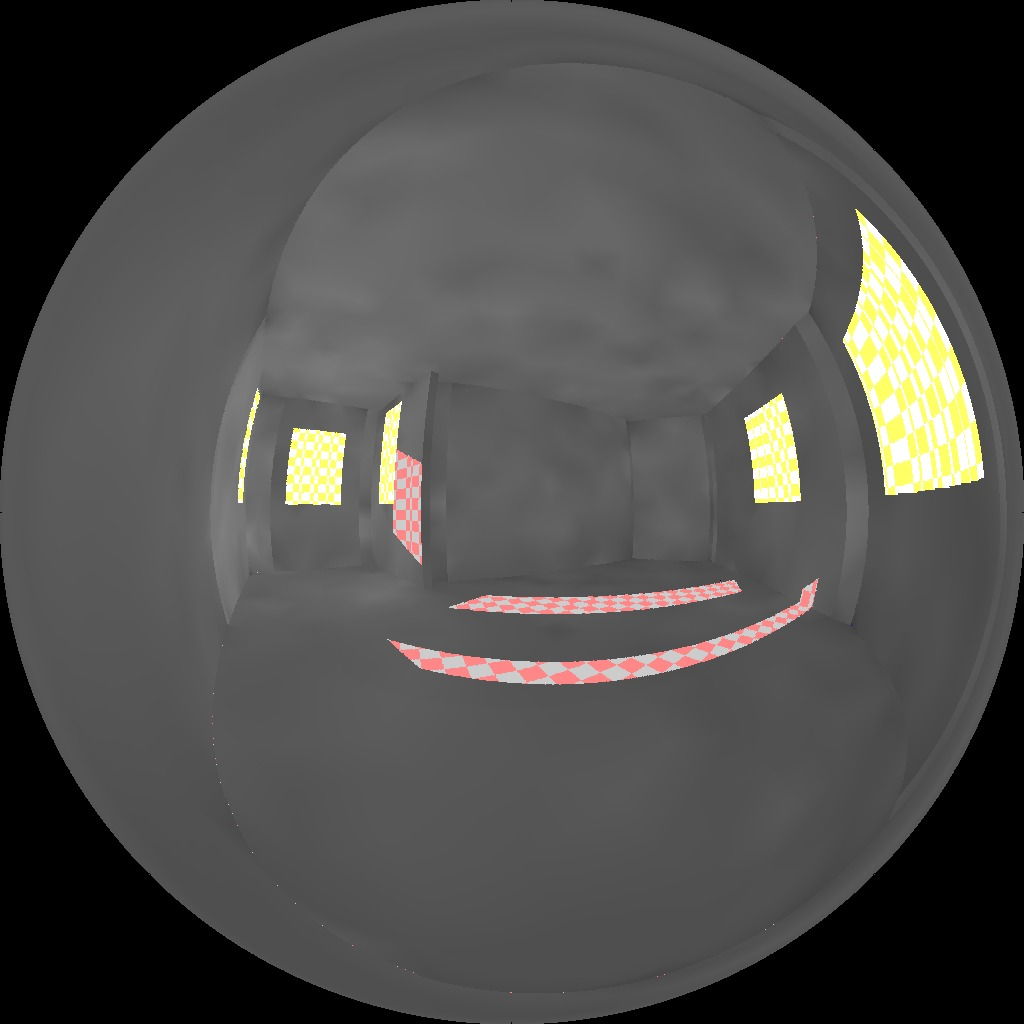
\includegraphics{wallfiles/classroom_2PM/surface_camera_VIEW_person4.jpg}}
%\resizebox{\picwidth}{!}{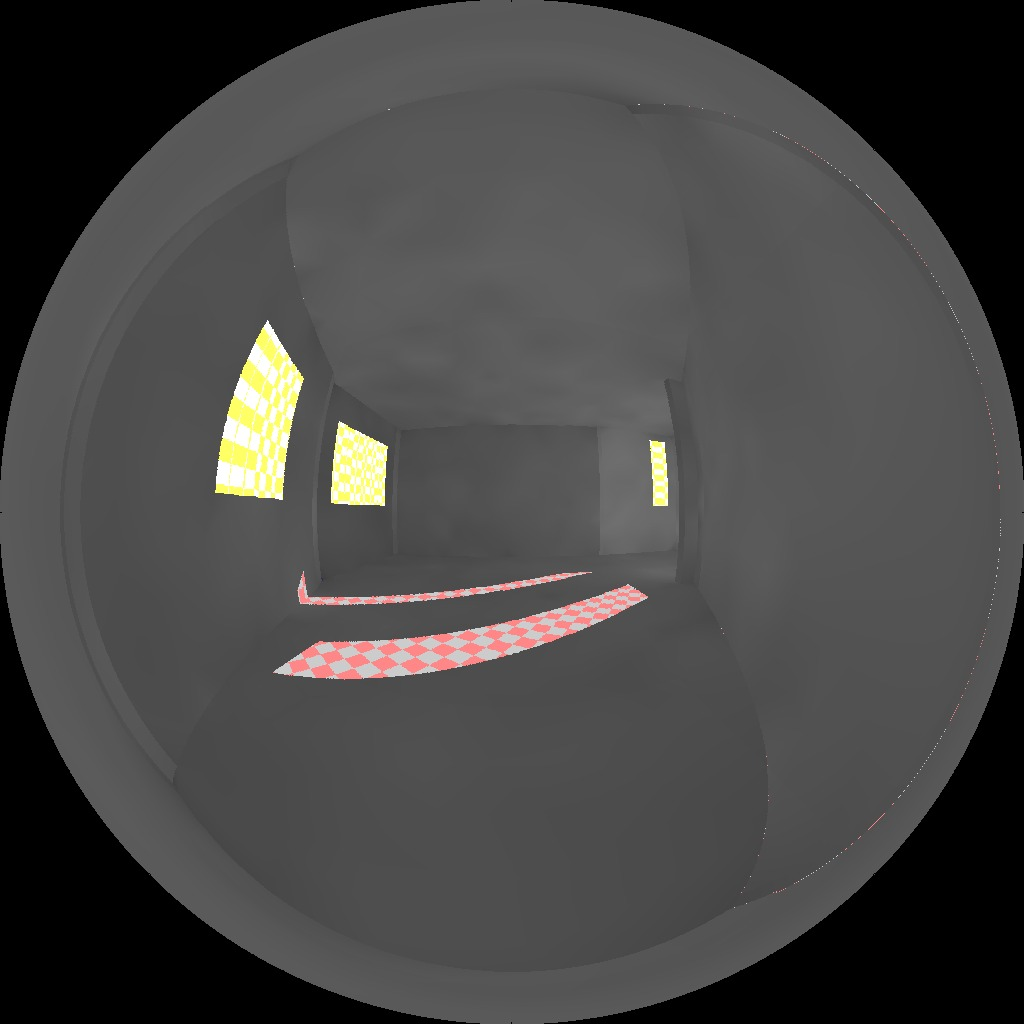
\includegraphics{wallfiles/classroom_2PM/surface_camera_VIEW_person5.jpg}}
%\vspace{-0.1in}
\resizebox{\picwidth}{!}{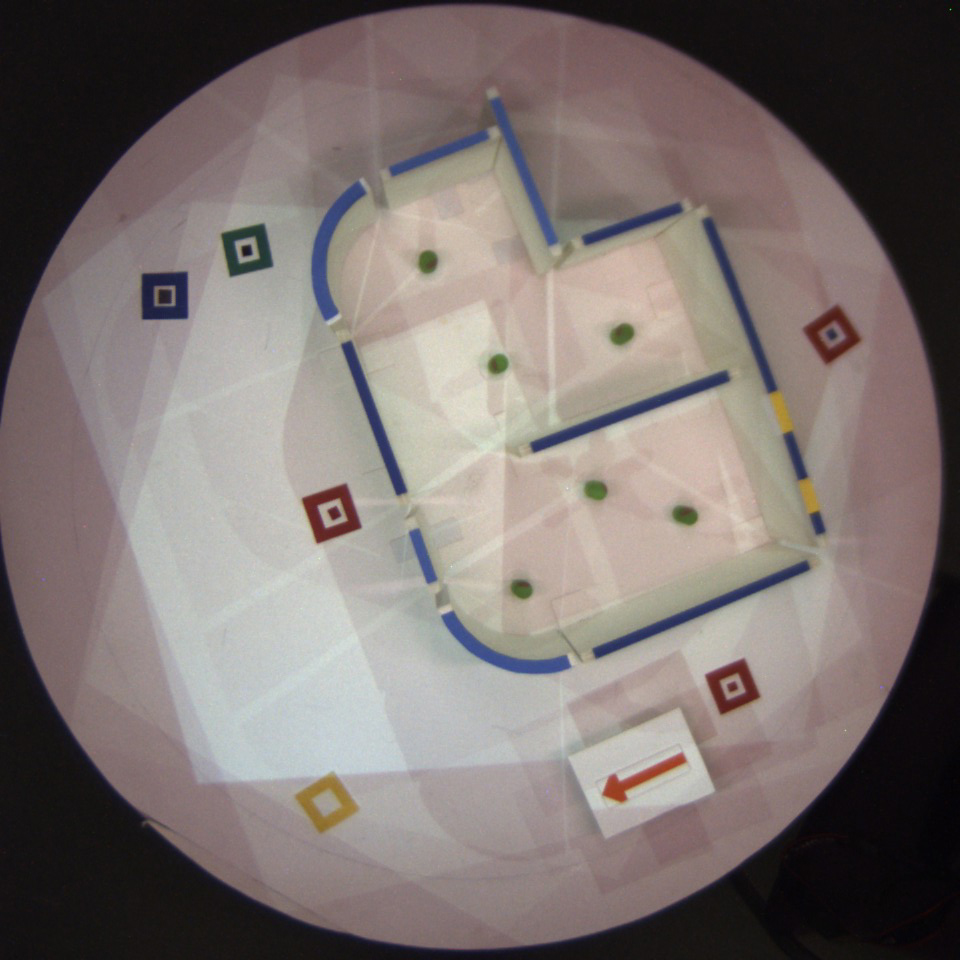
\includegraphics{wallfiles/mrc331/out_rotated.jpg}}
%
\hfill
\resizebox{\picwidth}{!}{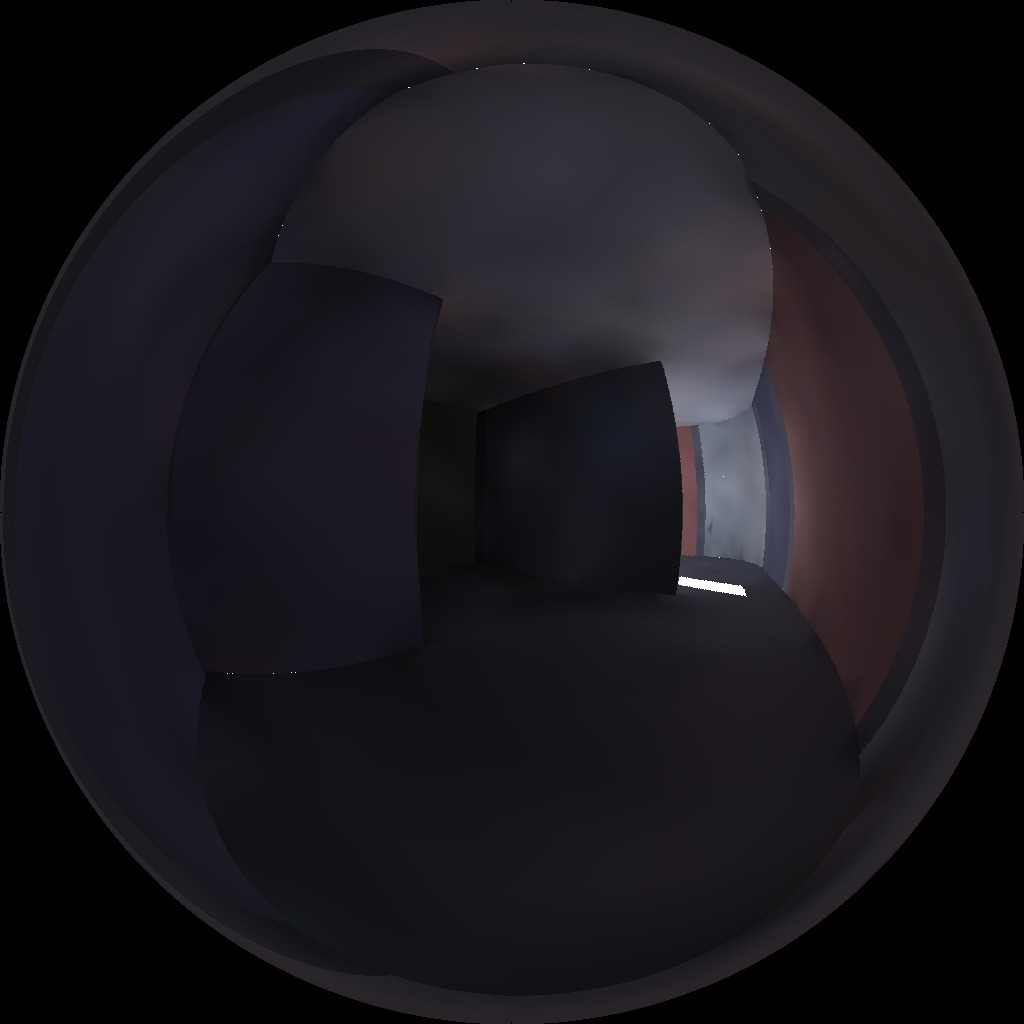
\includegraphics{wallfiles/mrc331_real_color/surface_camera_VIEW_person0.jpg}}
\resizebox{\picwidth}{!}{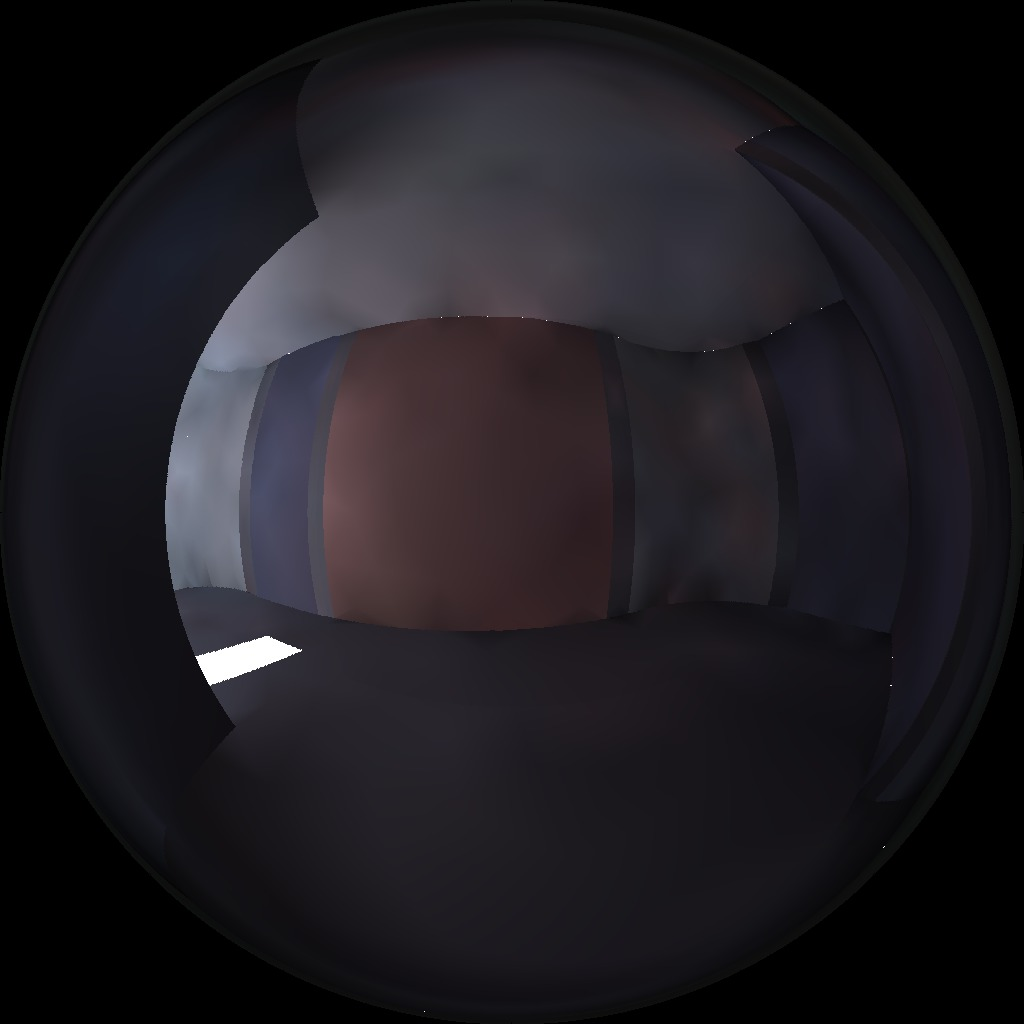
\includegraphics{wallfiles/mrc331_real_color/surface_camera_VIEW_person1.jpg}}
\resizebox{\picwidth}{!}{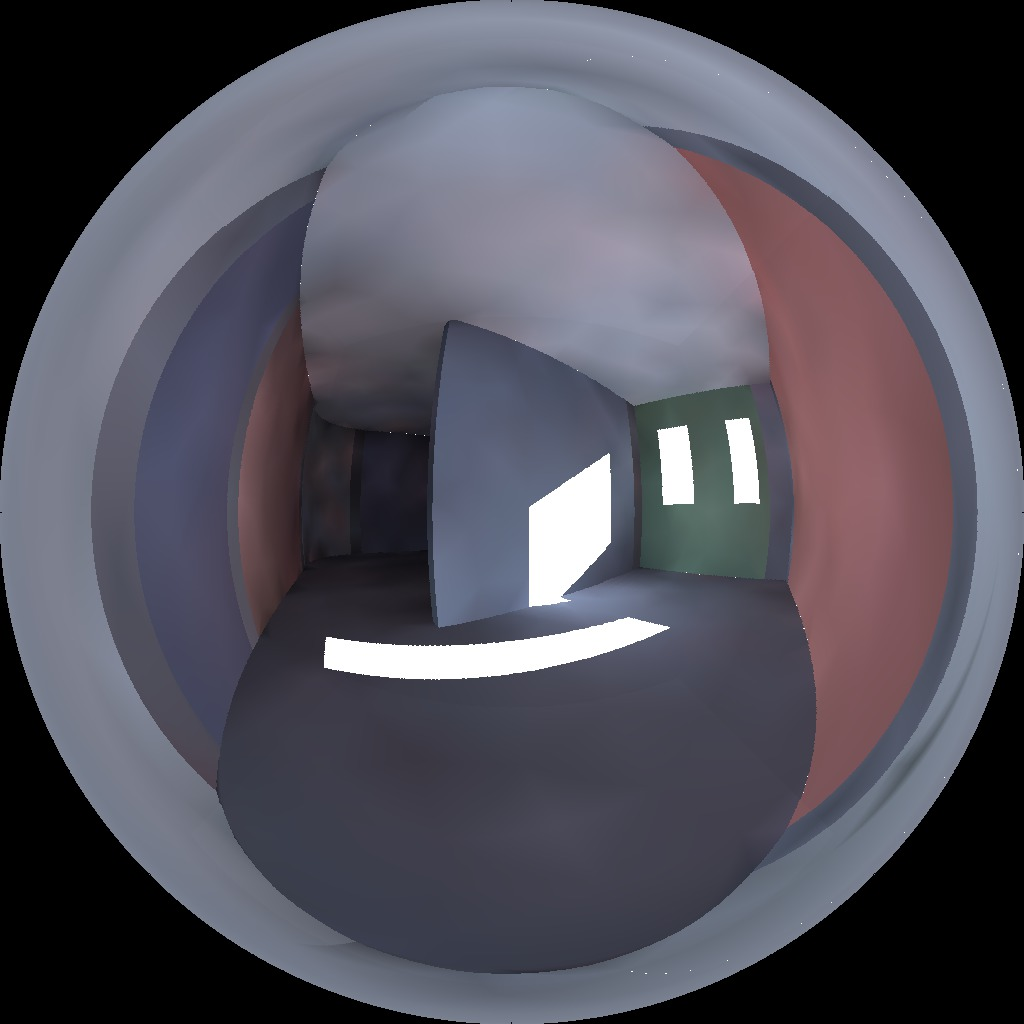
\includegraphics{wallfiles/mrc331_real_color/surface_camera_VIEW_person2.jpg}}
\resizebox{\picwidth}{!}{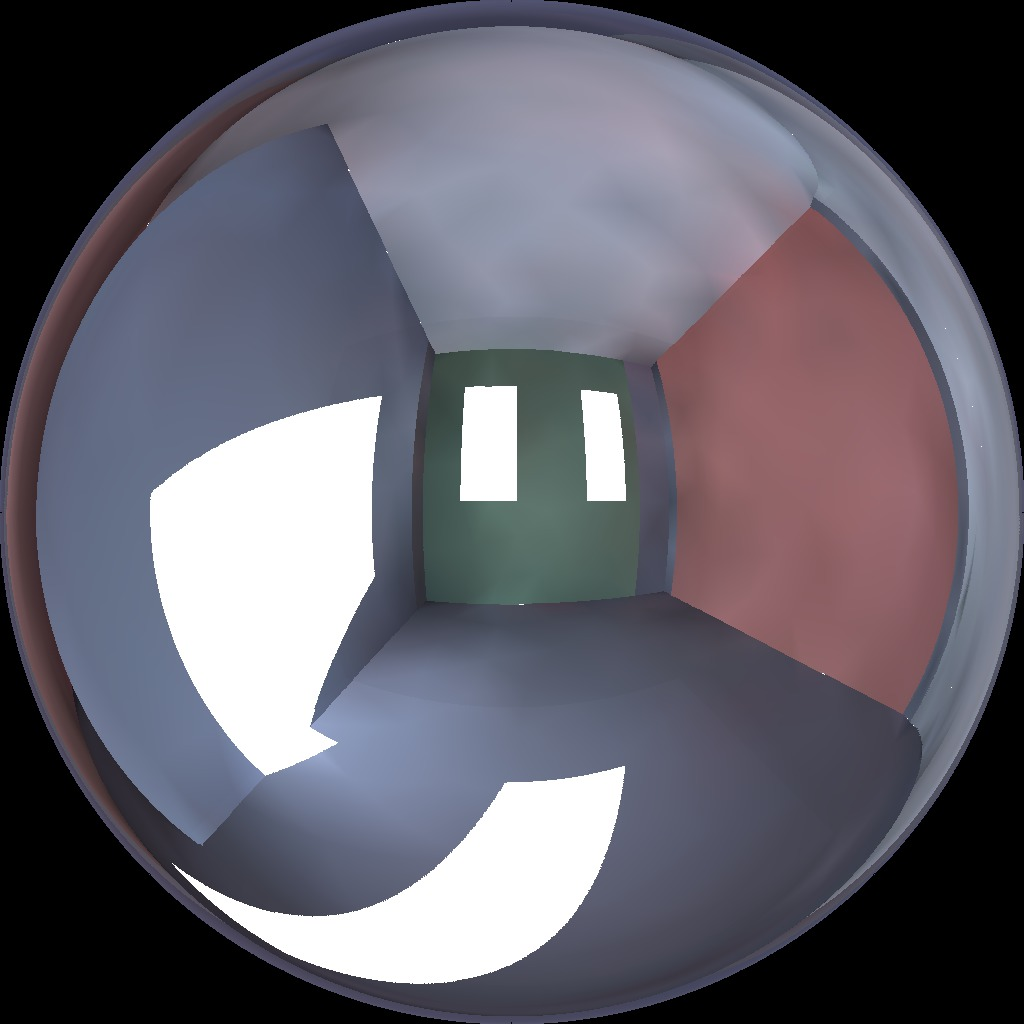
\includegraphics{wallfiles/mrc331_real_color/surface_camera_VIEW_person3.jpg}}
\resizebox{\picwidth}{!}{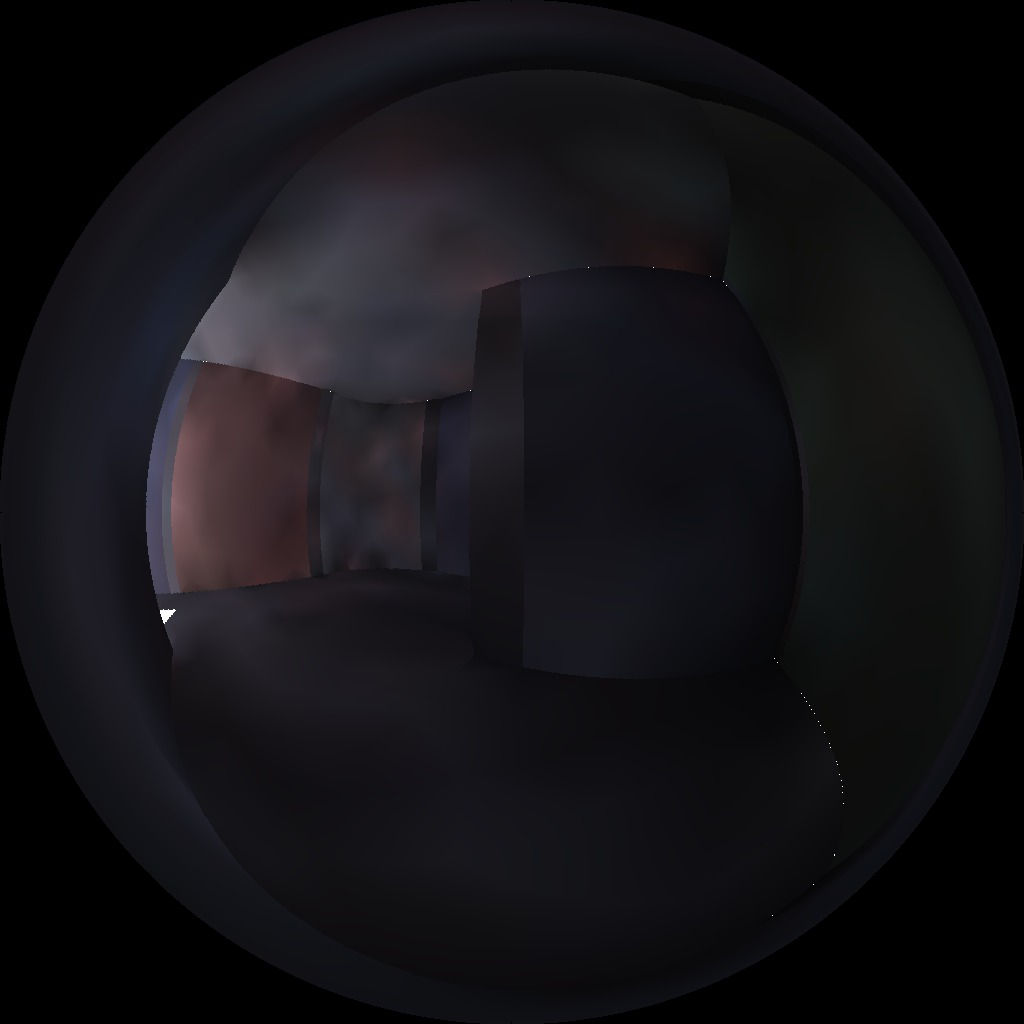
\includegraphics{wallfiles/mrc331_real_color/surface_camera_VIEW_person4.jpg}}
\resizebox{\picwidth}{!}{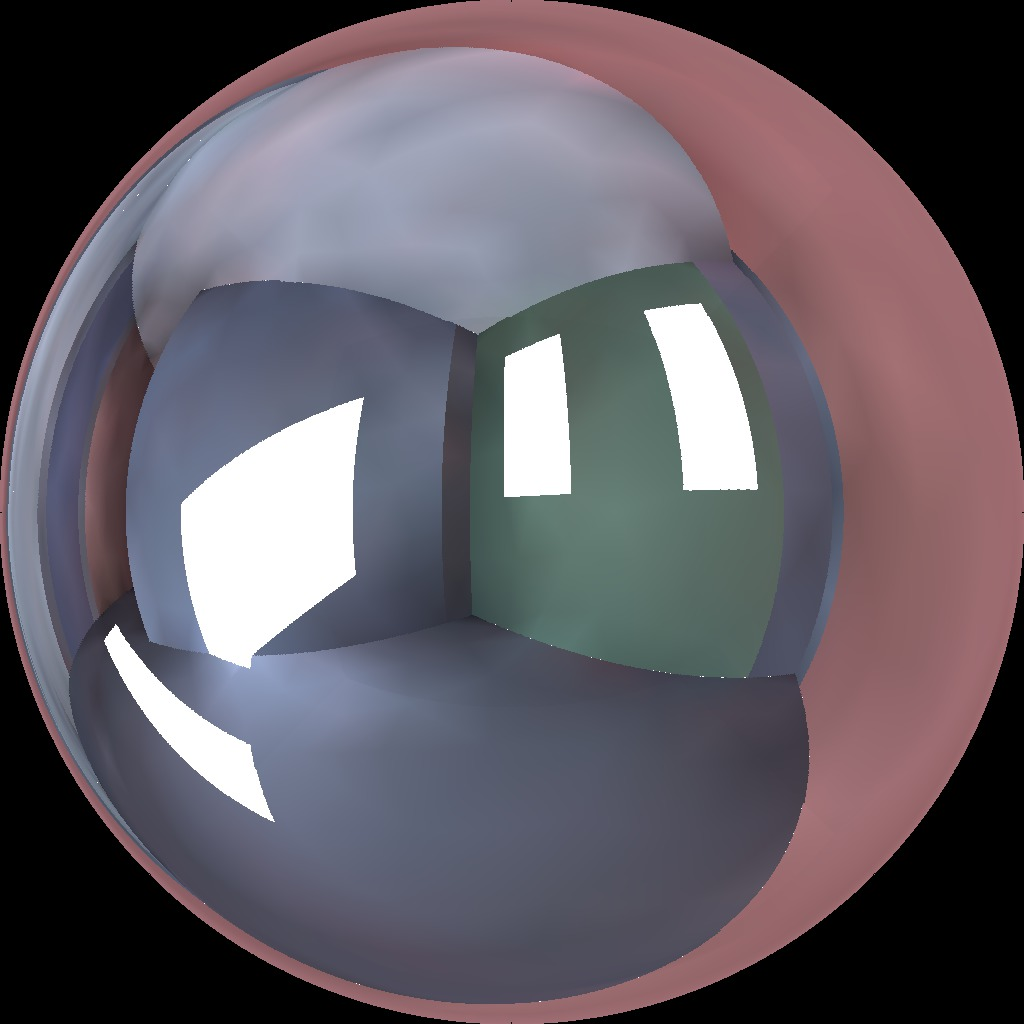
\includegraphics{wallfiles/mrc331_real_color/surface_camera_VIEW_person5.jpg}}\vspace{-0.15in}\\

\hfill
\resizebox{\picwidth}{!}{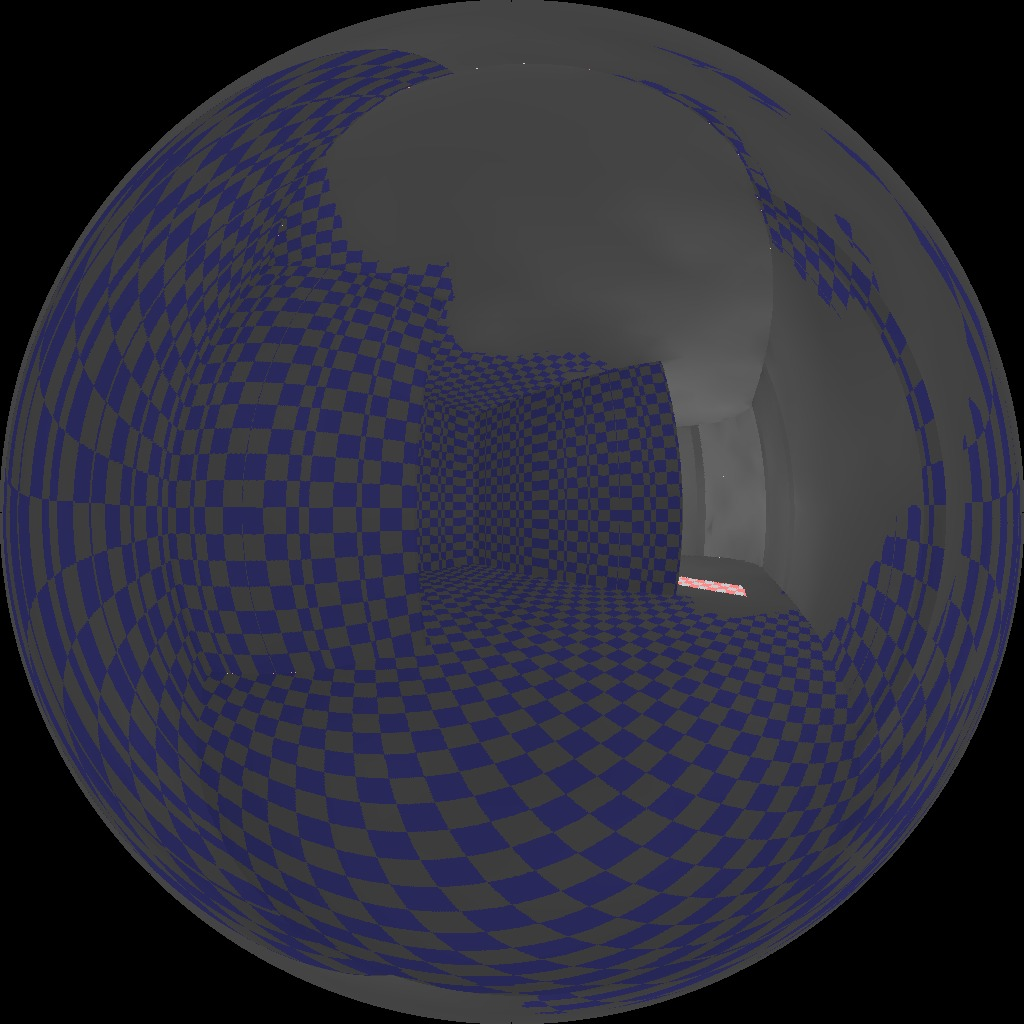
\includegraphics{wallfiles/mrc331/surface_camera_VIEW_person0.jpg}}
\resizebox{\picwidth}{!}{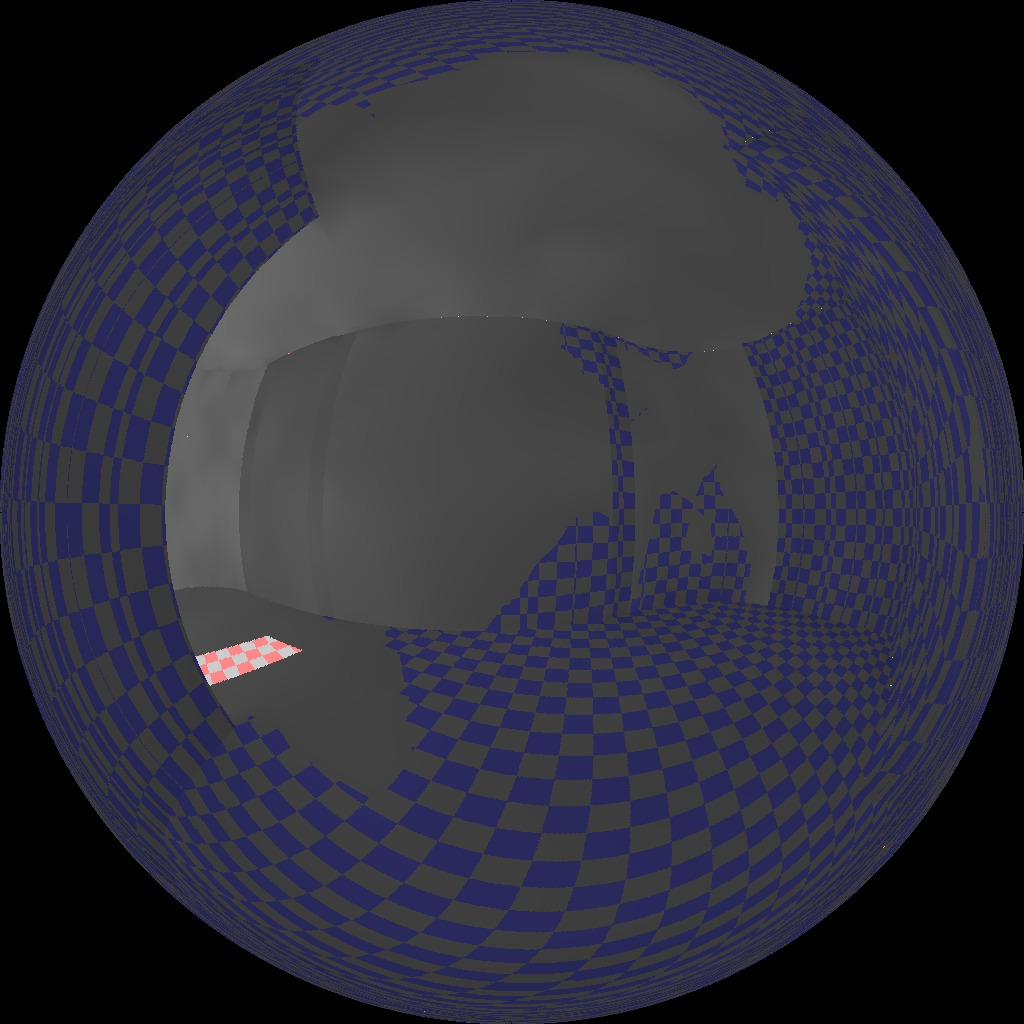
\includegraphics{wallfiles/mrc331/surface_camera_VIEW_person1.jpg}}
\resizebox{\picwidth}{!}{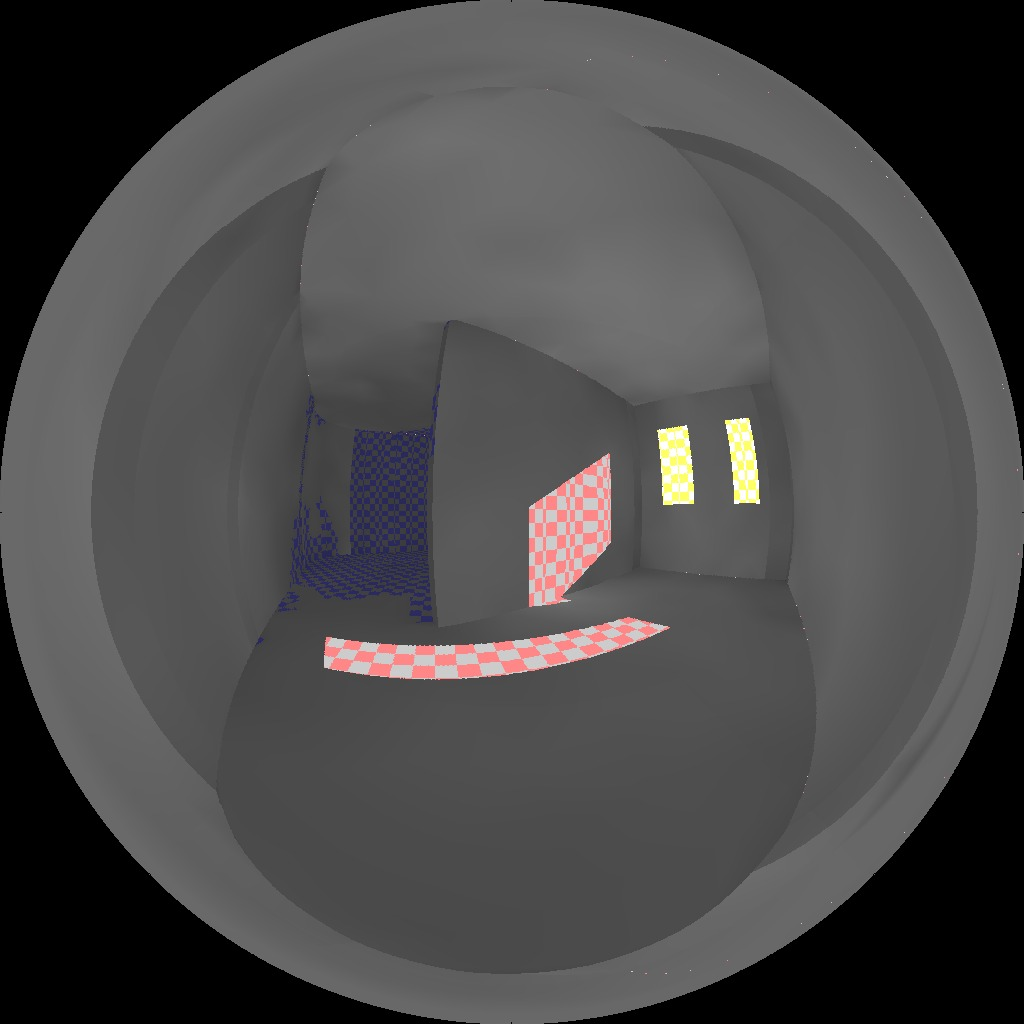
\includegraphics{wallfiles/mrc331/surface_camera_VIEW_person2.jpg}}
\resizebox{\picwidth}{!}{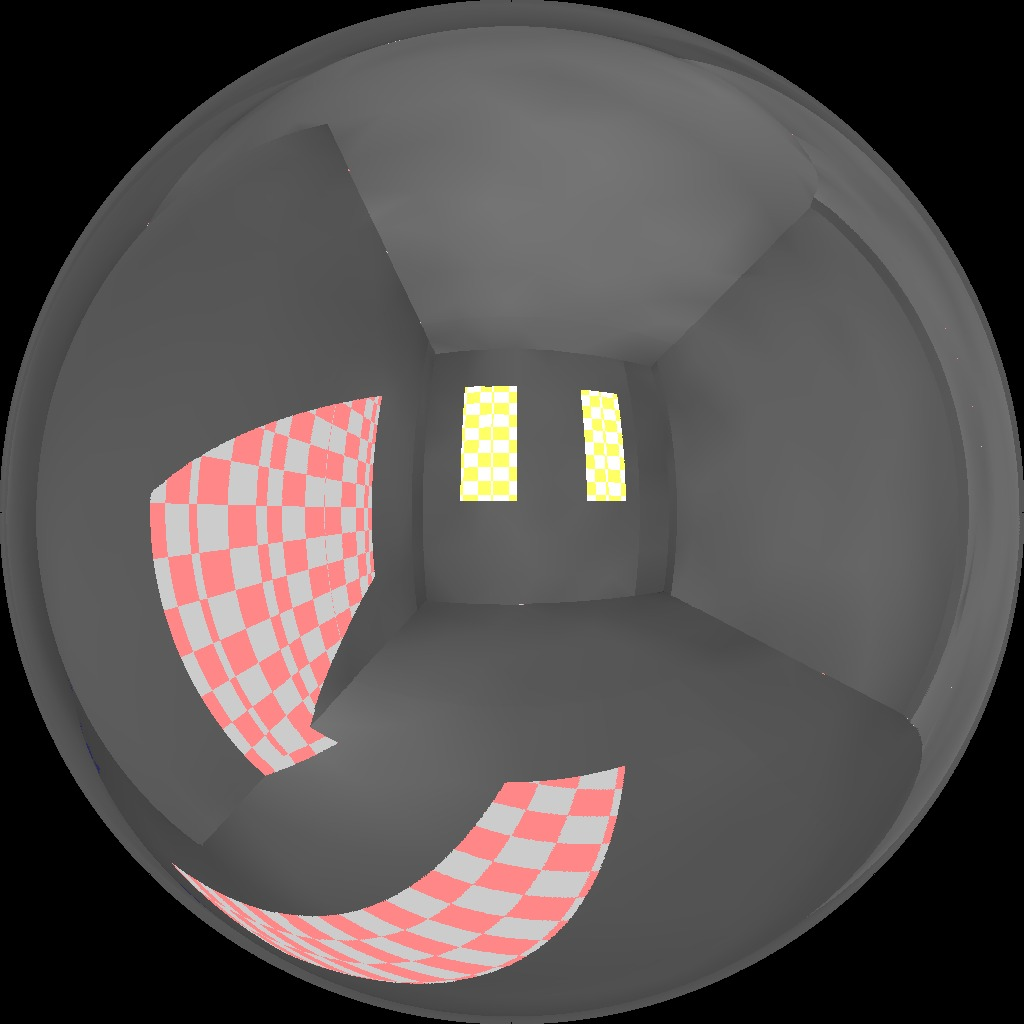
\includegraphics{wallfiles/mrc331/surface_camera_VIEW_person3.jpg}}
\resizebox{\picwidth}{!}{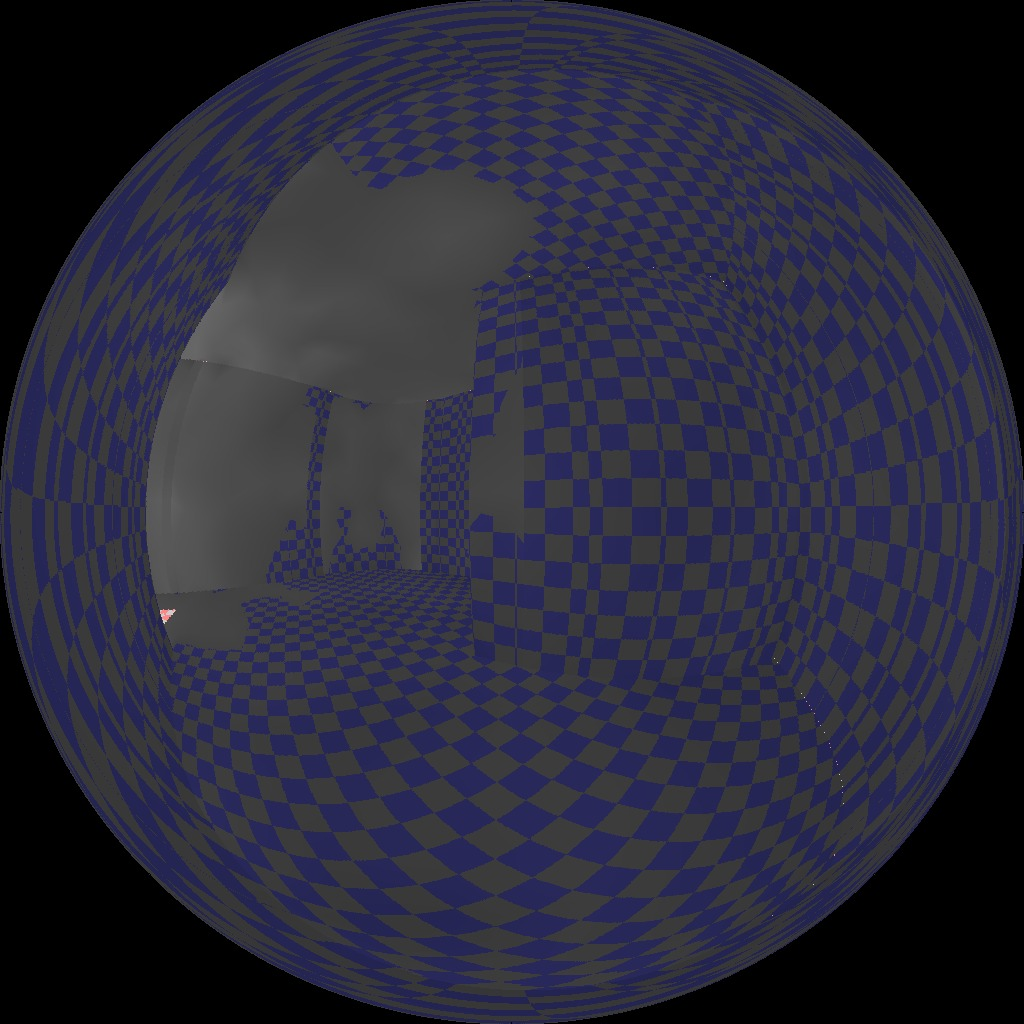
\includegraphics{wallfiles/mrc331/surface_camera_VIEW_person4.jpg}}
\resizebox{\picwidth}{!}{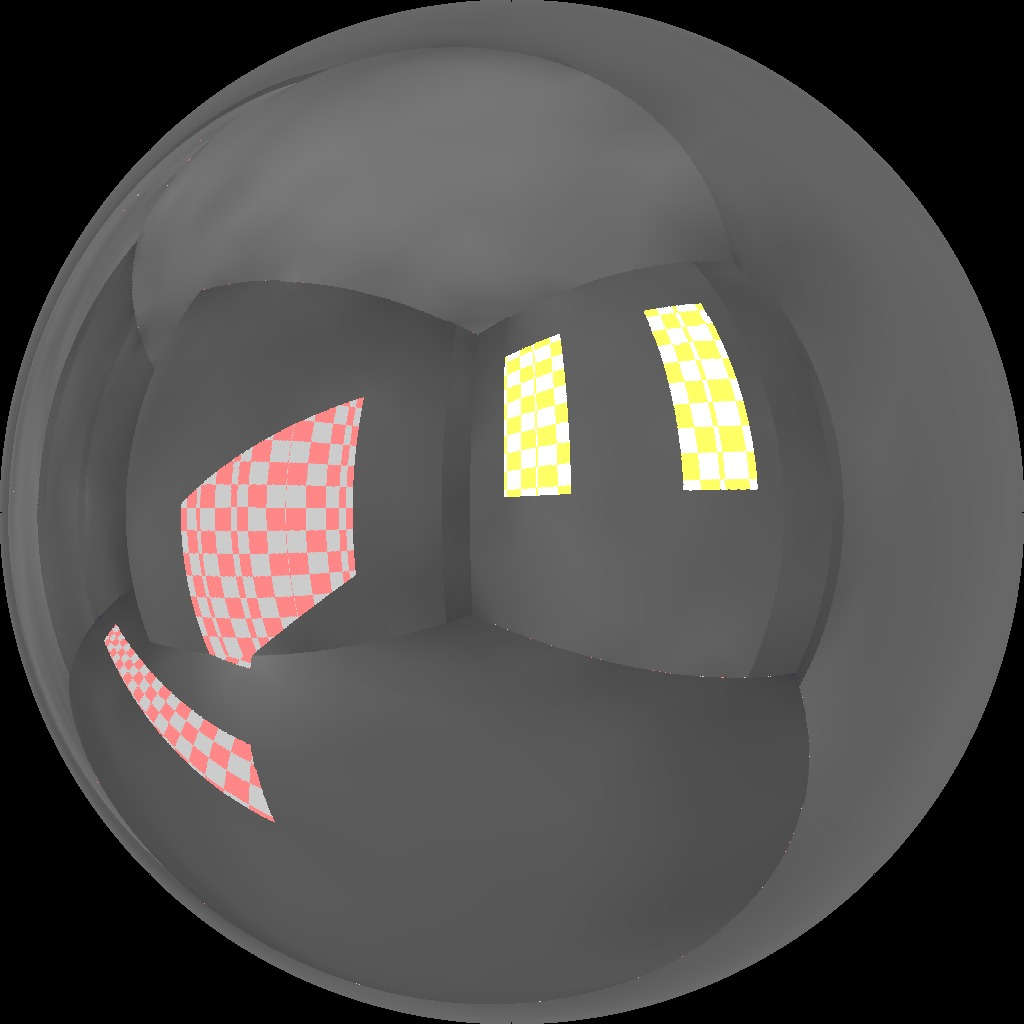
\includegraphics{wallfiles/mrc331/surface_camera_VIEW_person5.jpg}}
\caption{Fisheye views rendered from the position and orientation of
  each avatar token provide a visual perspective of the occupants of the design space
and immerse the users in the problematic over- and under-illumination conditions 
  of the office environment
in Figure~\ref{FIGURE:office_false_color}.  Illumination problems can
  vary significantly across different perspectives within the same
  space.}
\vspace{-0.15in}
\label{FIGURE:fisheyes}
\end{figure*}



\begin{figure*}[t]
\begin{center}
\newcommand{\picheight}{1.83in}
\newcommand{\picwidth}{\picheight}
%\resizebox{\picheight}{!}{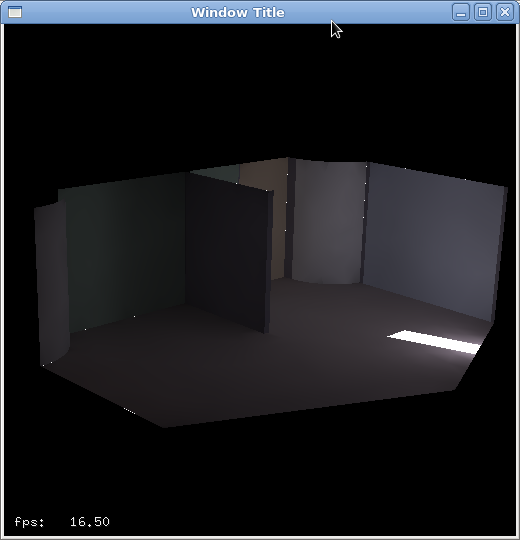
\includegraphics{wallfiles/cool_floor/cool_floor_normal_render.png}}
%\resizebox{\picheight}{!}{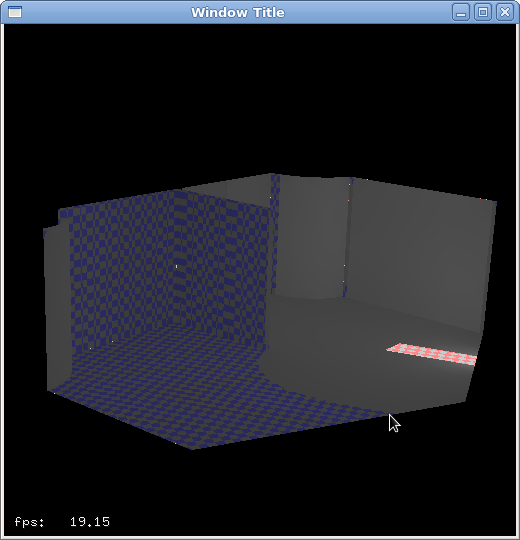
\includegraphics{wallfiles/cool_floor/cool_floor_false_color.png}}
%\raisebox{0.9in}{
\resizebox{\picwidth}{!}{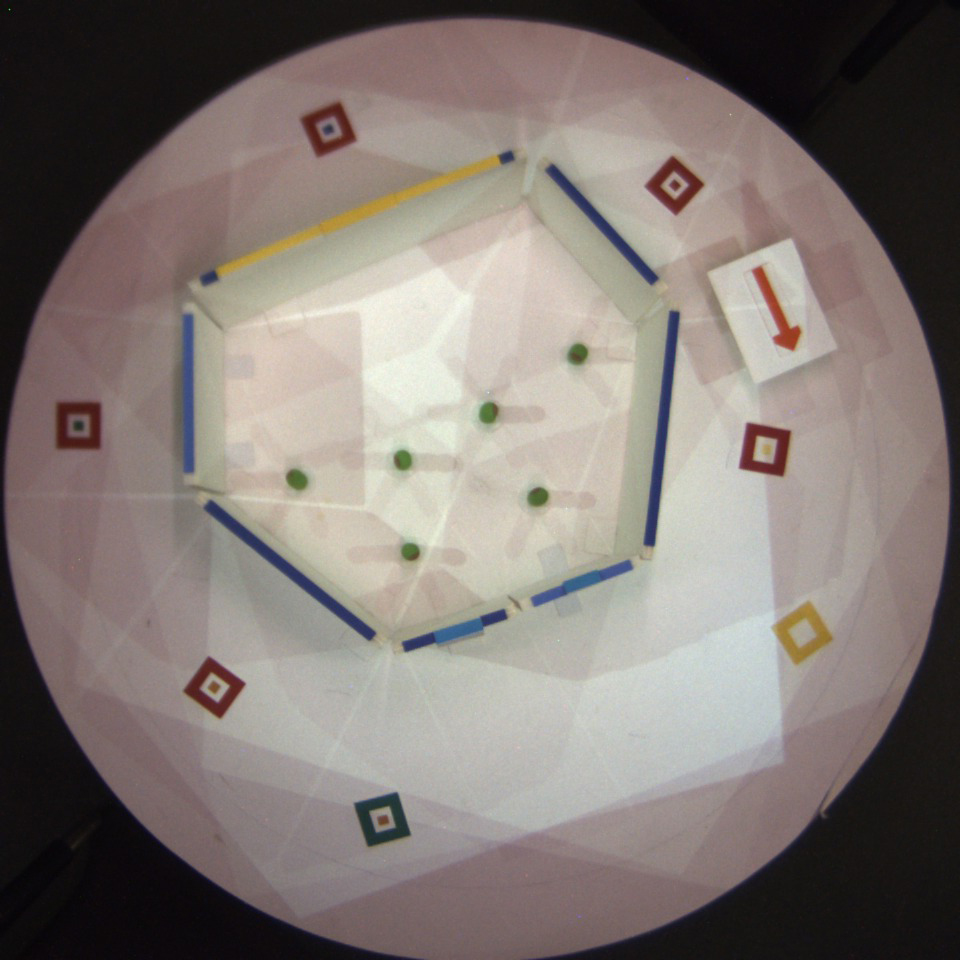
\includegraphics{wallfiles/museum2_false_nocurved/out_rotate.jpg}}
%}
\resizebox{!}{\picheight}{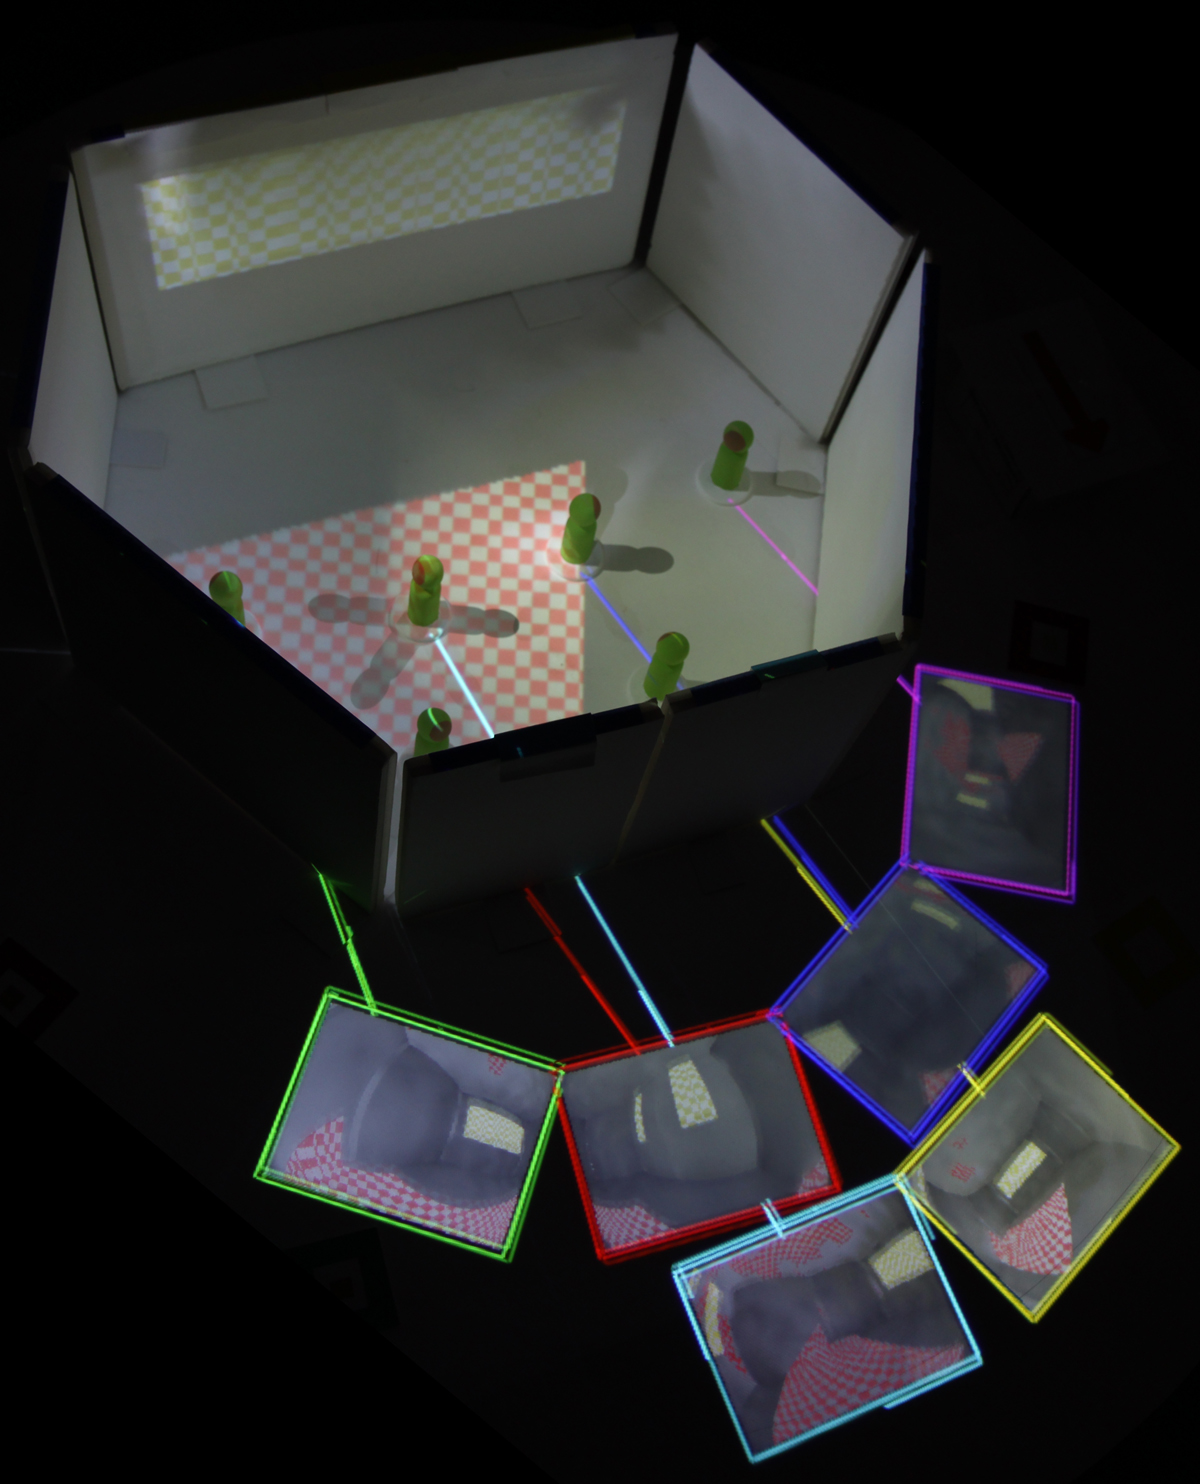
\includegraphics{photos/museum_false_color_nocurved.jpg}}
%\resizebox{\picheight}{!}{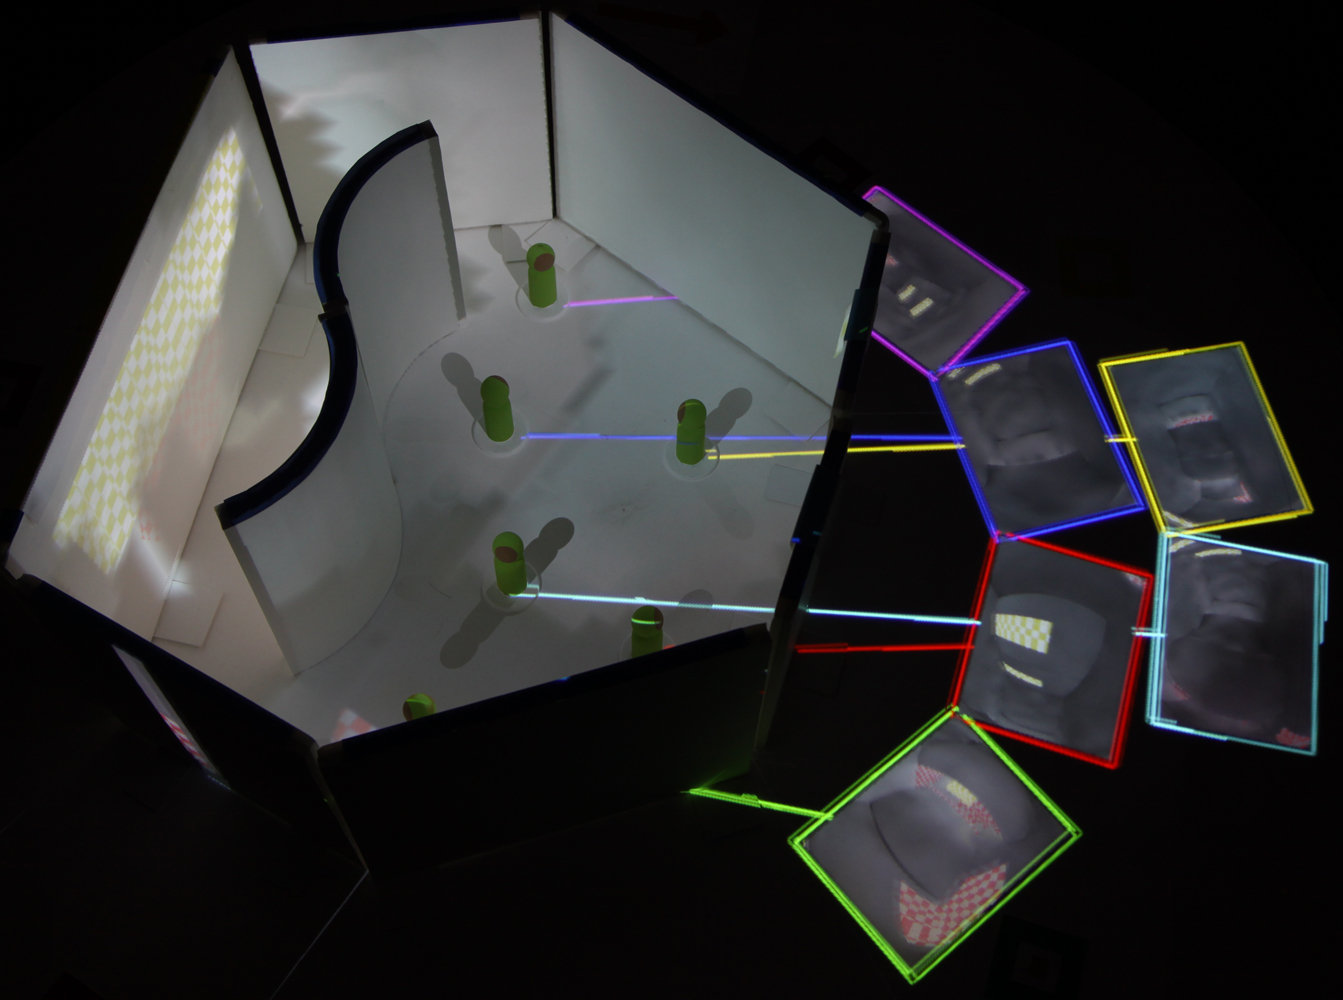
\includegraphics{photos/museum_false_color_curved.jpg}}
%
%\raisebox{0.9in}{
\resizebox{\picwidth}{!}{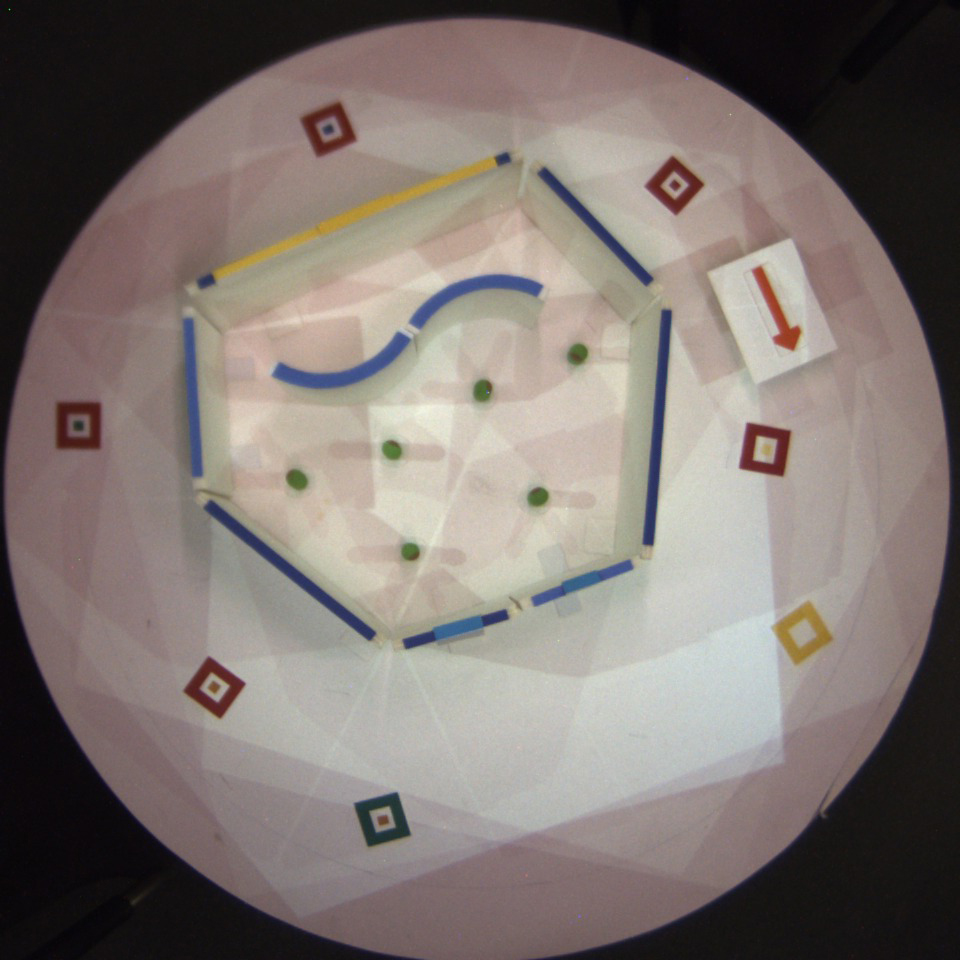
\includegraphics{wallfiles/museum2_false/out_rotate.jpg}}
\resizebox{!}{\picheight}{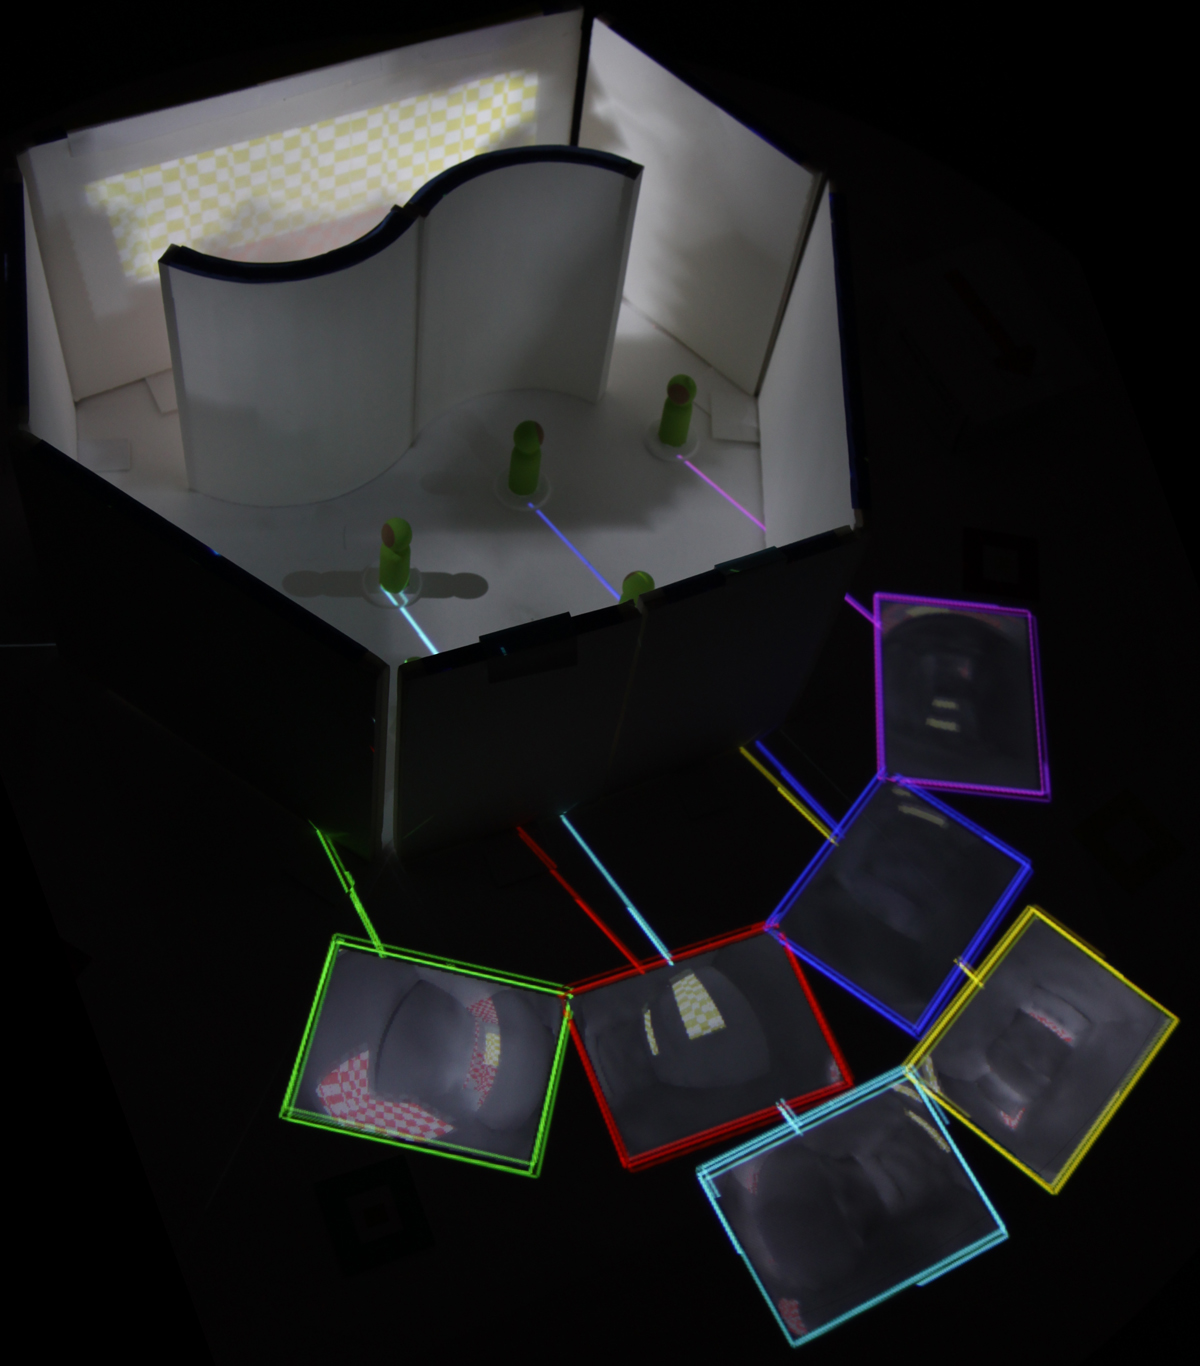
\includegraphics{photos/museum_false_color2.jpg}}
%}
%
\vspace{-0.1in}
\end{center}
\caption{ The left two images show an initial design proposal for an
  art gallery.  The rendering in the room and the glare views both
  show significant over-illumination and glare problems.  The right
  two images present a redesign that includes an interior curved wall
  to add visual interest and indirectly reflect the bright sunlight to
  reduce glare. The renderings of the room from each avatar are shown
  in Figure~\ref{FIGURE:museum2}.}
%
%The most common problem users encountered in our user study
%  was determining the areas that were too bright or too dark.  Our
%  false color visualizations will help future user discern where the
%  problem areas are.  The blue checkerboard is the under-illuminated
%  area and the red checkerboard is the over-illuminated area.
%
%}
%\vspace{-0.15in}
%\label{FIGURE:cool_floor}
\label{FIGURE:editing_model}
\end{figure*}





\begin{figure*}[t]
\newcommand{\picwidth}{1.12in}
%
\resizebox{\picwidth}{!}{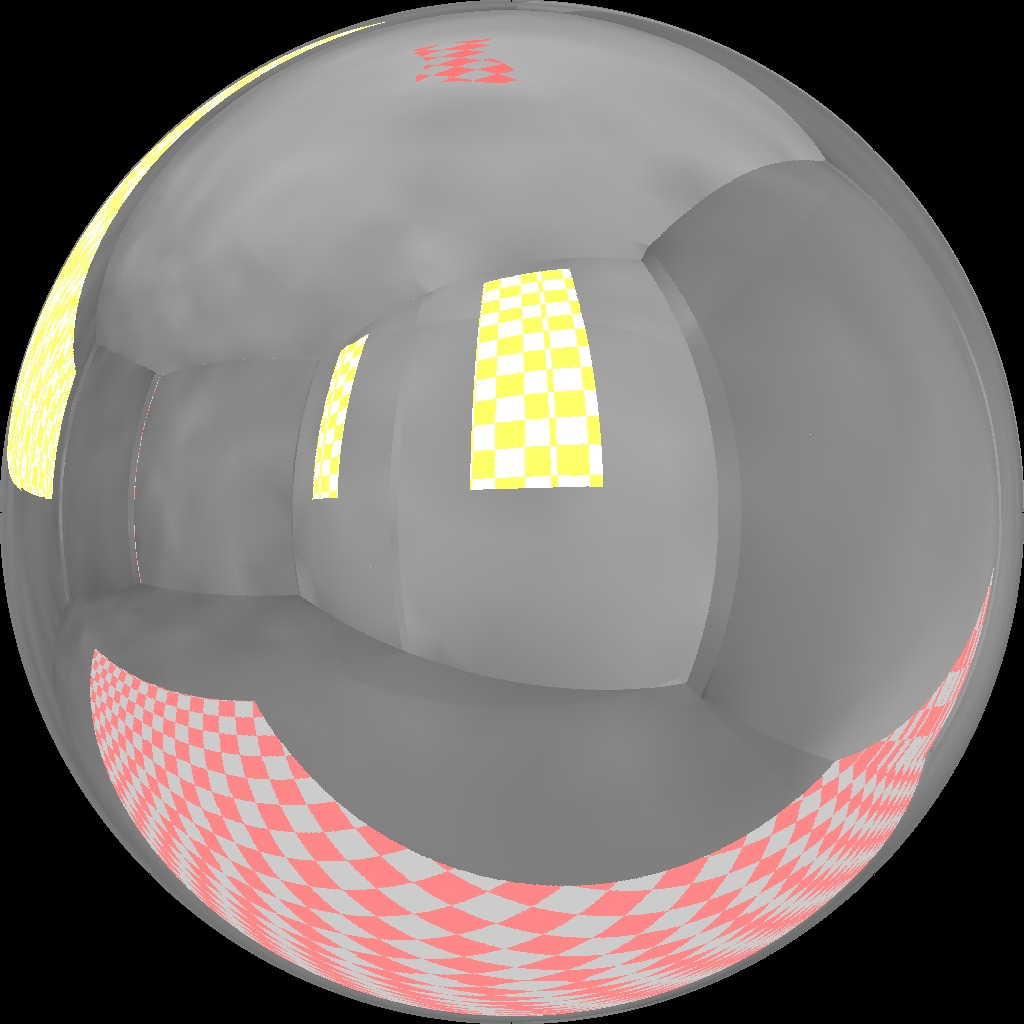
\includegraphics{wallfiles/museum2_false_nocurved/surface_camera_VIEW_person0.jpg}}
\resizebox{\picwidth}{!}{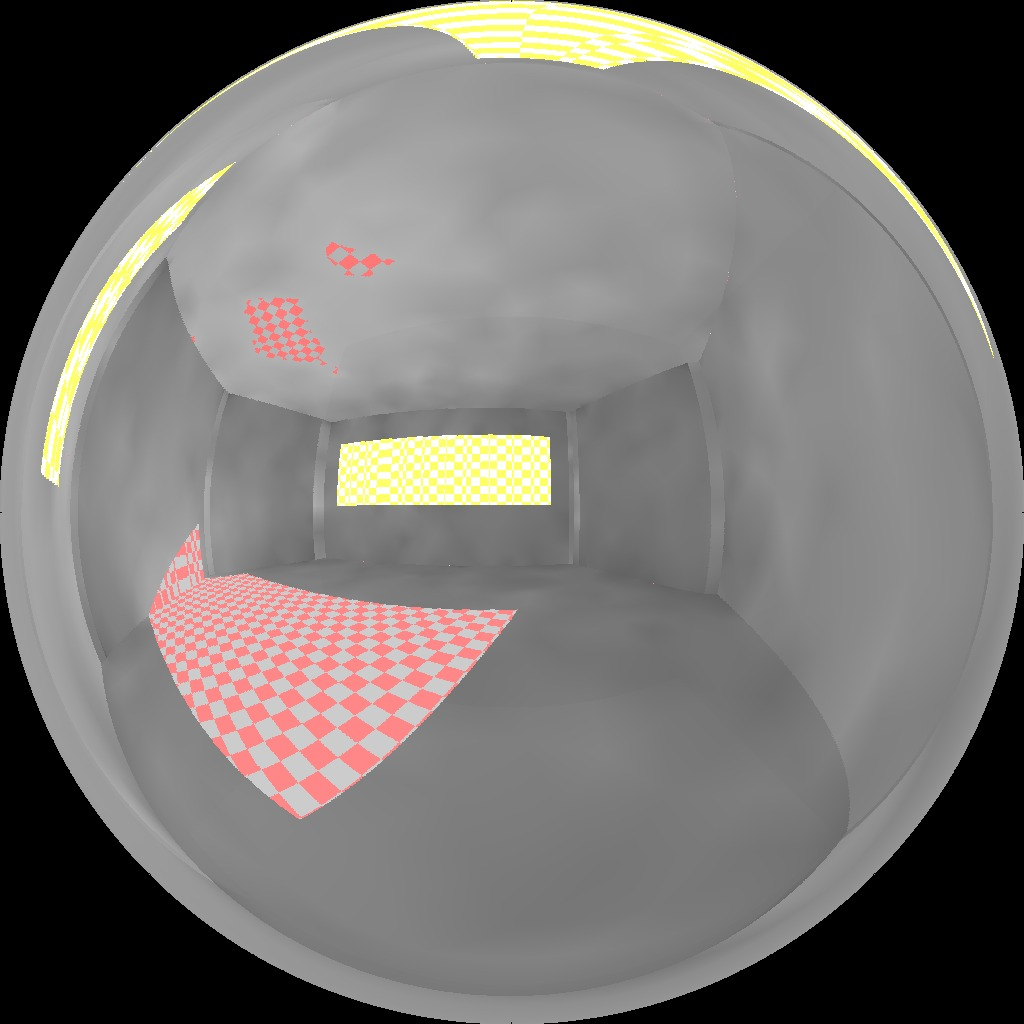
\includegraphics{wallfiles/museum2_false_nocurved/surface_camera_VIEW_person1.jpg}}
\resizebox{\picwidth}{!}{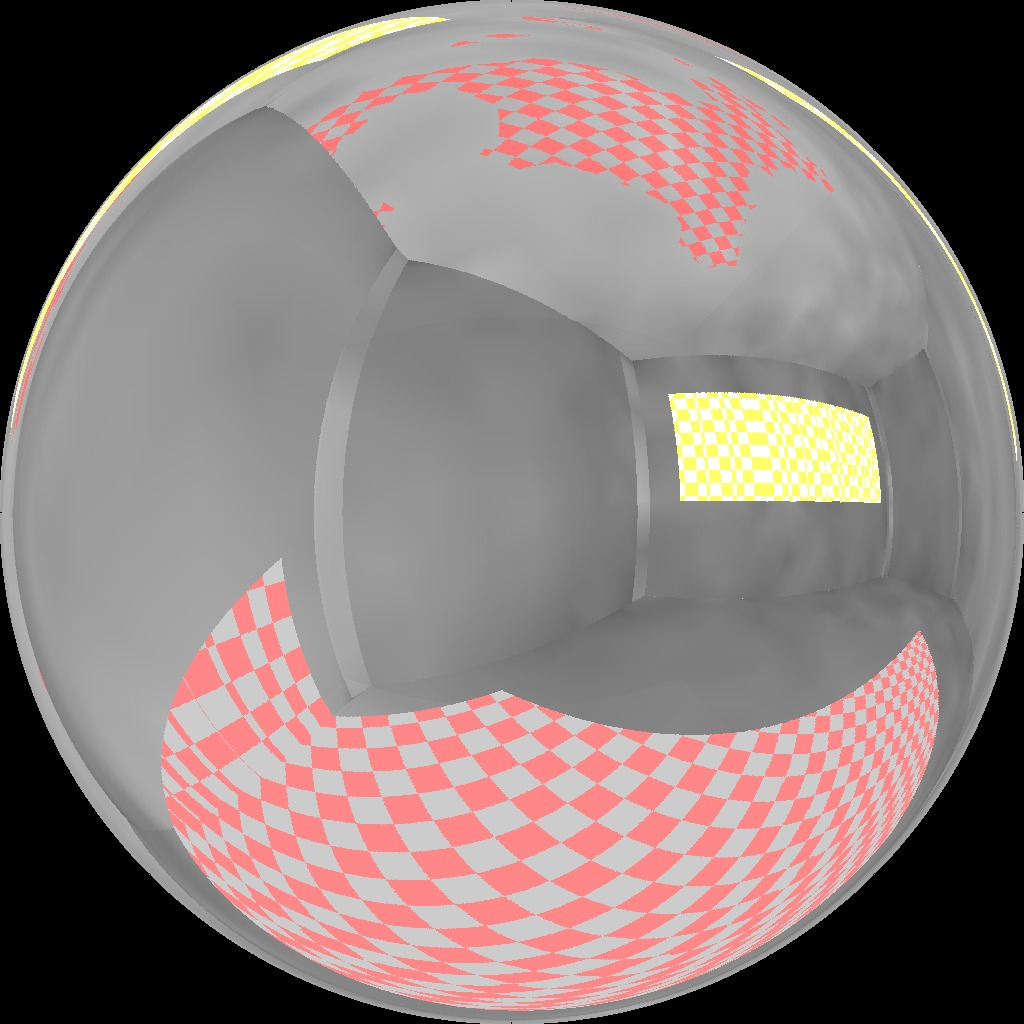
\includegraphics{wallfiles/museum2_false_nocurved/surface_camera_VIEW_person2.jpg}}
\resizebox{\picwidth}{!}{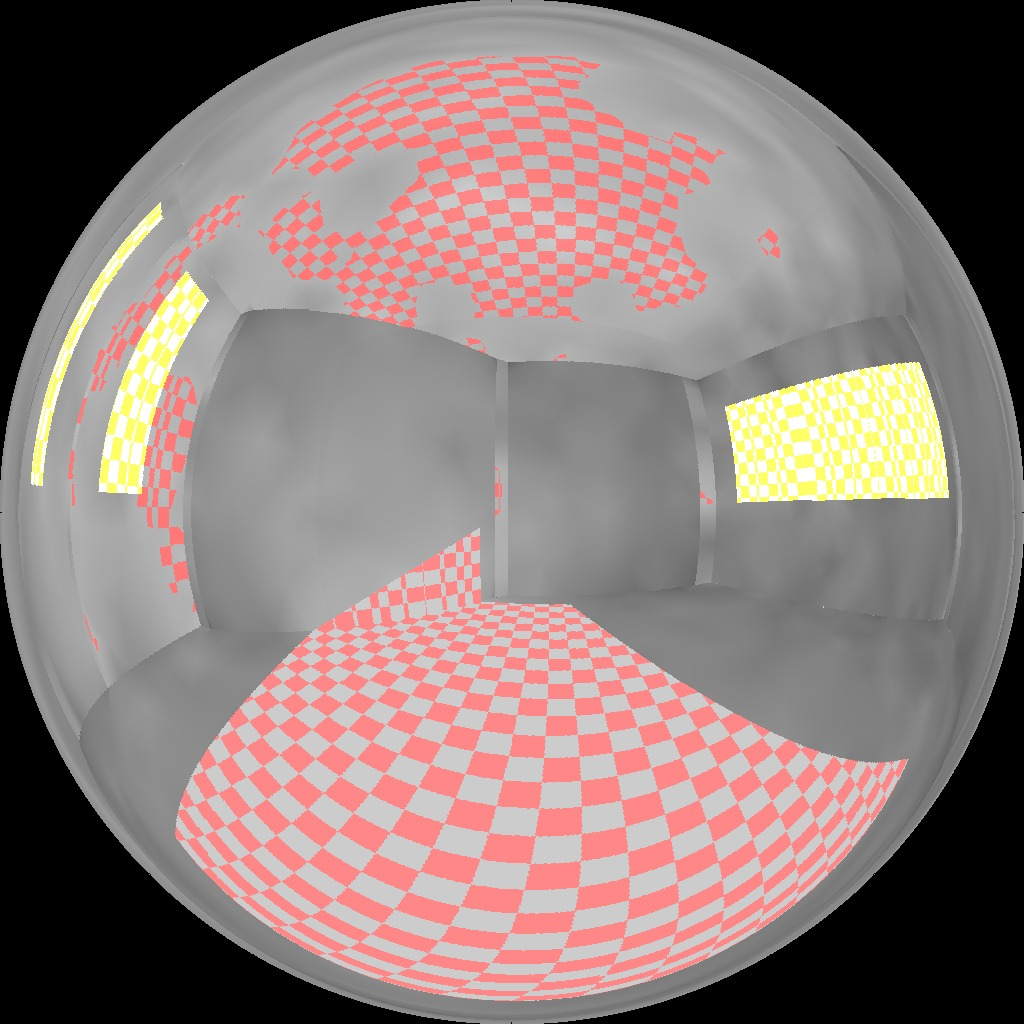
\includegraphics{wallfiles/museum2_false_nocurved/surface_camera_VIEW_person3.jpg}}
\resizebox{\picwidth}{!}{\includegraphics{wallfiles/museum2_false_nocurved/surface_camera_VIEW_person4.jpg}}
\resizebox{\picwidth}{!}{\includegraphics{wallfiles/museum2_false_nocurved/surface_camera_VIEW_person5.jpg}}
\\
\resizebox{\picwidth}{!}{\includegraphics{wallfiles/museum2_false/surface_camera_VIEW_person0.jpg}}
\resizebox{\picwidth}{!}{\includegraphics{wallfiles/museum2_false/surface_camera_VIEW_person1.jpg}}
\resizebox{\picwidth}{!}{\includegraphics{wallfiles/museum2_false/surface_camera_VIEW_person2.jpg}}
\resizebox{\picwidth}{!}{\includegraphics{wallfiles/museum2_false/surface_camera_VIEW_person3.jpg}}
\resizebox{\picwidth}{!}{\includegraphics{wallfiles/museum2_false/surface_camera_VIEW_person4.jpg}}
\resizebox{\picwidth}{!}{\includegraphics{wallfiles/museum2_false/surface_camera_VIEW_person5.jpg}}

%\vspace{-0.1in}
\caption{Fisheye views from each avatar in
  the gallery from Figure~\ref{FIGURE:editing_model}.  The top row shows each view for
  the initial design (which includes significant glare problems).  The
  bottom row shows the design from the same viewpoints after the re-design to reduce glare.}
\vspace{-0.15in}
\label{FIGURE:museum2}
\end{figure*}



%\subsection{Photon mapping}

In the rendering method used in our system, light is simulated
bouncing through the scene through the use of \emph{photons}.  Photon
Mapping is a method where photons are sent from a light source,
allowed to bounce around a scene and then gathered at specific
locations throughout the scene in order to be
rendered\cite{Jensen:1996:GIU:275458.275461}.  Image space photon
mapping was a GPU-accelerated version of photon mapping which allowed
interactive rendering time \cite{mcguire09imagespace}.  Our renderer
is based on an extension of this photon mapper which began
investigating how to use the sun and sky as a light source for image
spaced photon mapping \cite{ericli}.



\section{Motivation: Functional Architecture}

Rendering has traditionally been a field where generating an
aesthetically pleasing image has higher priority than
physical accuracy.  In architectural design, physical accuracy is just
as important as the appearance of the rendering.  Knowing the
locations suffering from over-illumination, under-illumination, and
glare directly impacts how useful a space is to potential occupants.
In spaces like art galleries, this is particularly relevant as direct
sunlight can damage artwork.  In a classroom, proper illumination is
important both so that students can read the chalkboard, books, and
laptops and so that the teacher and students can communicate
effectively.  Office environments need proper lighting because with
workers spending 40 hours per week on detailed tasks, employers must
ensure their safety and minimize fatigue and discomfort.  While
accurate simulation and measurement is important to creating a usable
and comfortable space, it is not sufficient to create an effective
design tool.  Architectural daylighting design is both the process of
admitting and redirecting an appropriate amount of light and making
creating aesthetic choices to create comfortable, beautiful, and
interesting spaces that offer healthy, productive, and inspiring work
and play environments.  Following these goals, we have also
incorporated the simulation of intricate screens to both control the
amount of light admitted through the windows and illustrate one way
our interface allows architects to create beautiful interior
environments.

%Rendering has traditionally been a field where generating an
%aesthetically pleasing image has been a higher priority than physical
%accuracy.  In architectural design, physical accuracy is just as
%important as the appearance of the rendering.  Knowing the locations
%suffering from overillumination, underillumination and glare directly
%impacts how useful a space is to potential occupants.  In spaces like
%art galleries, this is particularly relevant as direct sunlight can
%damage artwork.  While accuracy is important, it is not sufficient to
%create an effective renderer.  Architectural daylighting is both the
%process of choosing an appropriate amount of light and making creative
%aesthetic choices.  We chose to add intricate screens to the windows
%to illustrate one way our interface allows architects to make these
%choices.


\begin{figure*}[t]
\newcommand{\picwidth}{1.68in}
\resizebox{\picwidth}{!}{\includegraphics{wallfiles/mrc331/mrc331_6_21_7am_mod_crop.png}}
\resizebox{\picwidth}{!}{\includegraphics{wallfiles/mrc331/mrc331_6_21_11am_mod_crop.png}}
\resizebox{\picwidth}{!}{\includegraphics{wallfiles/mrc331/mrc331_12_21_7am_mod_crop.png}}
\resizebox{\picwidth}{!}{\includegraphics{wallfiles/mrc331/mrc331_12_21_11am_mod_crop.png}}%
%\vspace{-0.1in}
\caption{Over- and under-illumination are dynamic conditions and can vary drastically
  over a single day and throughout the year.  We present simulations for  June 21
  at 7 am, June 21 at 11 am, December 21 at 7 am, and December 21 at 11
  am.  Note that in June the over-illuminated regions are
  near the window, while in December most of the room
  experience over-illumination at some point in the day.  } 
\vspace{-0.05in}
\label{FIGURE:mrc331}
\end{figure*}

%\begin{figure*}[t]
%\newcommand{\picwidth}{.95in}
%\resizebox{\picwidth}{!}{\includegraphics{wallfiles/museum2_false_nocurved/out.jpg}}
%\resizebox{\picwidth}{!}{\includegraphics{wallfiles/museum2_false_nocurved/surface_camera_VIEW_person0.jpg}}
%\resizebox{\picwidth}{!}{\includegraphics{wallfiles/museum2_false_nocurved/surface_camera_VIEW_person1.jpg}}
%\resizebox{\picwidth}{!}{\includegraphics{wallfiles/museum2_false_nocurved/surface_camera_VIEW_person2.jpg}}
%\resizebox{\picwidth}{!}{\includegraphics{wallfiles/museum2_false_nocurved/surface_camera_VIEW_person3.jpg}}
%\resizebox{\picwidth}{!}{\includegraphics{wallfiles/museum2_false_nocurved/surface_camera_VIEW_person4.jpg}}
%\resizebox{\picwidth}{!}{\includegraphics{wallfiles/museum2_false_nocurved/surface_camera_VIEW_person5.jpg}}
%\\
%\resizebox{\picwidth}{!}{\includegraphics{wallfiles/museum2_false/out.jpg}}
%\resizebox{\picwidth}{!}{\includegraphics{wallfiles/museum2_false/surface_camera_VIEW_person0.jpg}}
%\resizebox{\picwidth}{!}{\includegraphics{wallfiles/museum2_false/surface_camera_VIEW_person1.jpg}}
%\resizebox{\picwidth}{!}{\includegraphics{wallfiles/museum2_false/surface_camera_VIEW_person2.jpg}}
%\resizebox{\picwidth}{!}{\includegraphics{wallfiles/museum2_false/surface_camera_VIEW_person3.jpg}}
%\resizebox{\picwidth}{!}{\includegraphics{wallfiles/museum2_false/surface_camera_VIEW_person4.jpg}}
%\resizebox{\picwidth}{!}{\includegraphics{wallfiles/museum2_false/surface_camera_VIEW_person5.jpg}}

%\vspace{-0.1in}
%\caption{This museum space model had significant glare problems.  By adding a curved wall in the middle, the glare problems are significantly reduced }
%\vspace{-0.15in}
%\label{FIGURE:museum2}
%\end{figure*}

\section{User Study of the Daylighting TUI}

We conducted a study to test users' evaluation of natural
lighting in existing spaces, their ideas for renovation of the space,
and the construction of a new design using our tools.  To accomplish
this, the participants visited an office space that has significant
over- and under-illumination problems.  We asked the users to make a
sketch on paper and use their intuition to describe the lighting
problems.
%
After completing their initial observations, the users built a
physical sketch of the space using our TUI daylighting system.  The
participants then used the system to evaluate lighting in the space by
requesting simulations and visualizations of multiple times throughout
the year and time-lapse animations.
%
The participants then edited their physical sketch to 
%We then requested that the users 
propose a minor renovation (e.g., changing the window configuration
and moving interior walls) and re-evaluated the natural lighting in
the space.
%
Finally, the participants
%we requested that the users 
created a new design from scratch with good daylighting principles
applied.  Once again they could use the system for renders and adjust
as necessary.

Users appreciated the simplicity of the design process.  We predicted
that users would be able to sketch and modify more quickly with our
design tool and that was validated by users successful designs and
post-study survey comments.
%
However, for the specific task of developing a renovation plan to
improve lighting in the space, most users focused solely on the
under-illumination problem and thus increased the south-facing window
area in the space. 
%
% They commented on the under-illumination in the
%room and attempted to adjust for it.  
%
Only a few of the participants noted the glare problems in the space
and attempted to minimize over-illumination.
%
When the users created their own designs they were more creative in
their attempts to create functional daylighting environments, but many
designs still exhibited significant areas of under- and
over-illumination and users struggled to recognize the potential for
glare.

While users appreciated the ability to express their design ideas and
to incrementally redesign, their significant difficulties discerning
which regions were functionally too bright or too dark 
%for the space to be useful
motivated us to update the system.
%
Renovations usually made most of the space bright enough to work, but
created over-illumination in a large section of the room and created
significant glare problems for the occupants.  While our simulations
are physically accurate, it is impossible to reproduce the brightness
and contrast and high dynamic range of direct sunlight and shadow
within a spatially augmented reality environment built with
off-the-shelf low dynamic range projectors.  As a result, the
renderings on the tabletop are a scaled representation of sunlight in
the room similar to an image taken with a specified exposure.

\section{System Improvements for Effective Design}
%Over-illumination and Under-illumination}

% i know i asked for this section... but it is repetitive and we are out of space
%
%As a result of the user study, we determined that we should make additional
%system enhancements.  Because it was impossible to give users renderings
%which were as bright as the sun, we decided that it was necessary to provide 
%alternate rendering modes to our renderer.  We also wanted to provide users
%with more tools to reduce the intensity of light in problem areas.

%\fbox{ really should have transition paragraph here}

%\fbox{ the paragraph sections could be switched back to regular subsections... }

%\vspace{-0.1in}
\paragraph{Over-illumination and Under-illumination}

% for version
%of our Tangible User Interface for architectural design and
%daylighting simulation. 
%\fbox{OSHA standards}
%http://www.osha.gov/SLTC/etools/computerworkstations/wkstation_enviro.html#lighting
To communicate lighting problems more effectively, we added a false
color visualization that emphasizes areas in the room that are too
bright or too dark.  The thresholds for over- and under-illumination
are customizable.  The Occupational Safety \& Health Administration
(OSHA) recommends 20 to 50 foot-candles for a standard office
environment \cite{OSHA}.  We now show areas with a checkered pattern
that are over-illuminated (red) or under-illuminated (blue) and
additionally label the view through windows in the model with a yellow
checkerboard because these views often produce bright glare for the
user.  A checkered pattern is created by overlaying a checkerboard
grid with alternating grid cells of the color above and the original
illumination value in greyscale.  
%Examples of this visualization are
%shown throughout the paper.

%ring the image.
%
%
%Alternating checkers are colored.  
%The non-colored checkers are still the 
%the rendered illumination value in greyscale.% color.  
%


%in An example of this can be seen in figure \ref{FIGURE:mrc331}.
%In

We believe a solid color visualization would be sufficient in many
cases; however, there are situations where the visualization could be
hard to evaluate.  For example, in an elementary school classroom 
painted with bright colors, it could be very difficult to discern
the a simple overlaid color visualization.
%color visualized and green checkerboards in this environment.
Similarly, in places where there is significant over or under
illumination simply scaling a color channel may 
produce a noticeable visualization.  
%An alternate
%visualization mode is available where the rendering is presented in
%greyscale.
%
%but chose the checkerboard pattern 
%
%will be
%sufficient to communicate lighting problems in most simulations, there
%are situations where the visualization could be hard to evaluate.
%
Thus, we choose to preserve the rendered greyscale intensity gradient
in the alternate checkers so it is still possible to analyze the
brightness gradient
%darkest and brightest spots 
in these 
%extreme 
areas.
%
%The visualizations of over-illumination and
%under-illumination are still colored and the lighting information is
%still shown in a modified intensity, but the color information in the
%scene is omitted.  
Furthermore, this provides an opportunity for illumination to be
evaluated in spaces where the color is distracting from the
daylighting design task or where the problem spots in the room would
be too dark or too bright for our visualization to be easily seen.  In
Figure \ref{FIGURE:office_false_color}, there is an office space that
suffers from both overillumination and underillumination.  We hypothesize
that this 
%If we had
%provided this 
visualization will be of significant benefit to users of this interface.
%to our participants, it would have been
%clear which areas were over-illuminated and we hypothesize they could
%have made better design decisions as a result.  
We will test this visualization 
%%%%%intend to test this
%hypothesis 
in a future user study to confirm that participants are able to make
better design decisions with this new quantitative information.

We chose the checkerboard pattern over other visualization techniques
including using the temporal variation to convey information (e.g., a
blinking visualization).  
%We chose not to use the temporal axis
We need to preserve the temporal axis for the time-lapse daily
variation animation that is an important feature
%because one important feature of our system is the ability to show an
to visualize 
%animation which plays an animation of 
the dynamic lighting over the course of a day described in Sheng et
al.~\cite{ShengYYC09, sheng_TVCG}.

%\begin{figure*}[t]
%\newcommand{\picwidth}{.9in}
%\resizebox{\picwidth}{!}{\includegraphics{wallfiles/classroom_12PM/surface_camera_VIEW_person0.jpg}}
%\resizebox{\picwidth}{!}{\includegraphics{wallfiles/classroom_12PM/surface_camera_VIEW_person1.jpg}}
%\resizebox{\picwidth}{!}{\includegraphics{wallfiles/classroom_12PM/surface_camera_VIEW_person2.jpg}}
%resizebox{\picwidth}{!}{\includegraphics{wallfiles/classroom_12PM/surface_camera_VIEW_person3.jpg}}
%\resizebox{\picwidth}{!}{\includegraphics{wallfiles/classroom_12PM/surface_camera_VIEW_person4.jpg}}
%\resizebox{\picwidth}{!}{\includegraphics{wallfiles/classroom_12PM/surface_camera_VIEW_person5.jpg}}
%\\
%\resizebox{\picwidth}{!}{\includegraphics{wallfiles/classroom_2PM/surface_camera_VIEW_person0.jpg}}
%\resizebox{\picwidth}{!}{\includegraphics{wallfiles/classroom_2PM/surface_camera_VIEW_person1.jpg}}
%\resizebox{\picwidth}{!}{\includegraphics{wallfiles/classroom_2PM/surface_camera_VIEW_person2.jpg}}
%\resizebox{\picwidth}{!}{\includegraphics{wallfiles/classroom_2PM/surface_camera_VIEW_person3.jpg}}
%\resizebox{\picwidth}{!}{\includegraphics{wallfiles/classroom_2PM/surface_camera_VIEW_person4.jpg}}
%\resizebox{\picwidth}{!}{\includegraphics{wallfiles/classroom_2PM/surface_camera_VIEW_person5.jpg}}
%\vspace{-0.1in}

%\resizebox{\picwidth}{!}{\includegraphics{wallfiles/mrc331/out.jpg}}
%\resizebox{\picwidth}{!}{\includegraphics{wallfiles/mrc331/surface_camera_VIEW_person0.jpg}}
%\resizebox{\picwidth}{!}{\includegraphics{wallfiles/mrc331/surface_camera_VIEW_person1.jpg}}
%\resizebox{\picwidth}{!}{\includegraphics{wallfiles/mrc331/surface_camera_VIEW_person2.jpg}}
%\resizebox{\picwidth}{!}{\includegraphics{wallfiles/mrc331/surface_camera_VIEW_person3.jpg}}
%\resizebox{\picwidth}{!}{\includegraphics{wallfiles/mrc331/surface_camera_VIEW_person4.jpg}}
%\resizebox{\picwidth}{!}{\includegraphics{wallfiles/mrc331/surface_camera_VIEW_person5.jpg}}
%\caption{Fisheye views were provided at the position and view
%  direction of each glare avatar to allow the users to experience the
%  lighting problems from the perspective of inside the model.
%  Illumination problems can vary significantly across different
%  perspectives within the same space.}
%\vspace{-0.15in}
%\label{FIGURE:fisheyes}
%\end{figure*}

\begin{figure*}[t]
\newcommand{\picheight}{1.25in}
\resizebox{!}{\picheight}{\includegraphics{wallfiles/museum/islamic_crop.png}}
\resizebox{!}{\picheight}{\includegraphics{wallfiles/museum/islamic-fc_crop.png}}
\resizebox{!}{\picheight}{\includegraphics{wallfiles/mrc331/islamic_crop_window_white.png}}
\resizebox{!}{\picheight}{\includegraphics{wallfiles/mrc331/islamic-fc_crop.png}}
\caption{ We added complex geometry to our window model to enable
  users to make the space more visually compelling.  These materials allow users to
  reduce the amount of light streaming into the room while also making
  the lighting more interesting.}%\fbox{reget images}
\vspace{-0.15in}
\label{FIGURE:screens}
\end{figure*}


\vspace{-0.1in}
\paragraph{Glare Tokens}

%\fbox{discuss press a button and recalculated aspect}

In addition to over-illumination problems, we noted that many users of
our system inadvertently created glare problems in their models.  Only
a few of the users were able to successfully increase {\em indirect}
illumination using interior walls to diffusely re-direct bright
sunlight from south-facing windows.  We re-create a similar scenario
in the example shown
%Two users in our study tried to minimize glare in a
in Figure~\ref{FIGURE:editing_model}.  Unfortunately, only about 25\%
of the participants in our original study even attempted to reduce
over-illumination and glare in our system.  In addition to users not
being able to understand what was too bright, we believe that users
had difficulties predicting and evaluating the visual perspectives the
occupants would experience.  To address this, we added avatar tokens
to measure glare in the design.  These tokens specify the position and
view direction of people engaged in typical usage of the space.  These
tokens can be used to identify problems, and also to aid in
optimization of the design for its intended function.
%
%These tokens can be placed throughout the scene so that users
%can investigate problems in useful areas.  
%
Closeup views of these tokens are shown in Figure~\ref{FIGURE:teaser}.
When viewed from the overhead camera we can detect the location of
each token and also the orientation; that is, which direction the
token's ``face'' is looking.

We render fisheye views from the each avatar's position and
orientation.  Because users seldom require the entire tabletop surface
for their models, the renderings are automatically placed in the
under-utilized areas of the table.  
%When chosing the placement of
%these extra visualizations 
The algorithm considers the geometry of the sketched design and how
this geometry occludes the otherwise available areas for some of the
projectors.  Each token's rendering is connected to the associated
avatar by a uniquely colored line.  The user can thus design the
functionality of the room and specify the location of desks in an
office environment or placement of a painting in an art gallery.
Based on these renderings, users can modify their design to correct
the most significant problems.
%
When the design modules or avatars are moved, the projector-camera system is signaled to recapture the model, 
recompute the lighting in the scene, and update the visualization
display.
% (along with the new configuration
%of glare tokens if applicable).



%In addition to overillumination problems, we noted that many users of
%our system inadvertently created glare problems in their models.  Two
%users in our study tried to minimize glare in a similar method to
%figure \ref{FIGURE:teaser} C.  Unfortunately only about 25\% of our
%users attempted to minimize glare in our system.  We hypothesize that
%if users had been given a way to view perspectives from inside the
%model that they would have been able to better adjust for glare.  To
%address this, we added glare tokens to our system.  These tokens can
%be places throughout the scene so that users can investigate problems
%in useful areas.  We rendered the perspectives from a fisheye camera
%to enable a larger field of view than a traditional camera.  Glare can
%be experienced in peripheral vision which is wider than our standard
%camera.  Our cropped fisheye views give a more appropriate perspective
%to a user experiencing the space. We render each of the views of these
%tokens based both on the position and direction of the token.  Because
%users seldom use the entire tabletop surface for their models, the
%renderings are placed in the empty parts of the tabletop.  We allow
%the use of up to 6 tokens.  Each token's rendering is connected to the
%token by a line on the tabletop display.  This allows the user to pick
%interesting areas in the room for example the intended placement of a
%desk in an office or a painting in an art gallery.  Based on these
%renderings, users can adjust their model slightly if one area is a
%problem or redesign if there are significant problems.



Figure~\ref{FIGURE:fisheyes} illustrates a wide range of variation in
the lighting conditions for the occupants of an office environment similar to that used in our earlier use study.
%, the office has even more varied perspectives.  
Some users will find it difficult to perform detailed task work because the space is under-illuminated while others will be hampered by overillumination and glare.
%viewpoints that have both too much (second) and too little
%(first, third, and fifth) light to be useful.  
The usual reaction in a space like this is to close the blinds and
turn on the interior lighting.  These visualizations will impress upon the 
%should be
%sufficient for 
the architect the need for 
%to realize that a 
redesign to fully leverage natural illumination.
Figures~\ref{FIGURE:editing_model}~and~\ref{FIGURE:museum2}
present an art gallery with significant
glare issues before and after the placement of a large interior
partition to diffusely reflect the direct sunlight.  Prior to the
addition, most of the space suffered from severe over-illumination.
%The addition ofWe applied a technique of diffusing the light with curved walls,
%similarly to what two students did in the user study.  
You will notice that second row has significantly lower glare for all
but one token's perspective.  
%The renovation is also shown on the
%tabletop in 
%.  
We hypothesize that if users are given this method to directly view
interior perspectives, their final designs will be appropriately tuned
to the intended usage of the space.
%models that users create will be
%better adjusted to reduce glare problems.



%\fbox{what is this paragraph?} gone
%Allow architects to visualize the space in addition to getting
%accurate simulation results Rendering is done using a photon mapping
%method which uses direct light added to photons being gathered
%almost) uniformly across the scene.  This allows for detailed
%geometry in the windows to create a detailed rendering while lighting
%eing accurate in the scene.

\vspace{-0.1in}
\paragraph{Window Materials}

Users of our system had difficulty finding ways to minimize glare.  
While part of this is likely due to difficulties understanding illumination,
part of the problem could have been a lack of sufficient tools to 
limit illumination.  
%
One common method to direct illumination in a space is to modify the
window materials, e.g., diffusing shades, prismatic glass, or
reflective light shelves.  We have integrated support for complicated
window screens as shown in Figure~\ref{FIGURE:screens}.  These screens
are one example of a window material that can both provide a way to
reduce illumination and make the space more visually interesting.  Due
to the modular nature of our renderer, it will be straightforward to
add many other types of materials to the interface.


\section{Discussion \& Future Work}

The modular nature of our TUI and SAR system allowed us to integrate
the new false color visualization and avatar glare token features with
relative ease.  Extending of the detection algorithm for colored
primitives on the tabletop and additions to the shader-based rendering
engine are possible
%many extensions are
%possible to our system 
without the need to significantly alter the system.
%
%As discussed earlier, 
We will be exploring efficient simulation of a wider variety of window materials
and developing an appropriate tangible interface for specifying these materials.
%putting screens in the window is just one of
%many possible geometries that could be added to the windows.  Many
%other geometries including shutters, louvers, etcetera could be added; 
%although they would be more expensive to
%compute than shades.

Our informal presentation of the new system to potential users has
been promising, but our next major step will be a formal study to
confirm the effectiveness of the new features of our system and to
guide 
%$should be conducted to evaluate the effectiveness of recent
%additions to the system as well as any 
possible future improvements.  The series of studies we have
already conducted with this system has helped guide our research
endeavors.
%identify 
%Our past user study motivated
%many of our implemented and planned changes, but a formal user study
%has not yet verified the effectiveness of these changes.  
%This study
%will likely validate many of our changes so far and motivate revisions
%as well as additional enhancements.

As presented in \cite{Garstka_Peters_2004}, head tracking could be a
valuable addition to our system.  Head position tracking should be
relatively simple with a depth camera placed above the table facing
down.  Gaze recognition could be omitted as simply obtaining a view of
the full rendering from the user's perspective should be sufficient.
%
Head tracking provides several advantages.  Currently, the glare views
are placed around the table in areas that are most empty and visible
to the projectors.  Alternatively, we could place these visualizations
so they are most visible to the users' current location (both location
and 'up' orientation).
%show these visualizations on the side of the table with the user if
%the user's position was known. 
While not providing any new information, this would remove the
inconvenience of looking around the geometry or walking to the other
side of the table to view the glare perspectives.
%
Additionally it provides the ability to save \emph{screenshots} from
the user's current location.  A screenshot is a view towards the
center of the table from the perspective of the person's head.  When a
user requests a screenshot it will be saved in a session folder.  This
provides the user with a way to revisit lighting problems after the
session has concluded and a way to collaborate.  The user can send a
subset of these renderings to the client or to other architects to
show both potential problems with the space or to direct the client
attention to certain aspects of the design.


\section{Conclusion}

Our enhancements to tabletop spatially augmented reality provide novel
and interesting interaction techniques in a projector-camera system.
These enhancements directly address problems revealed in a previous
user study of the system.  The false color visualizations in addition
to the greyscale mode of rendering provide an intuitive and easy way
to see when there are over- and under-illumination issues.  In addition
we provide a proof of concept for more complicated window designs by
providing the users with screens in the windows when requested.  The
glare token provides an exciting new way to communicate specific visual
perspectives of being in the space to the user.  Finally, we propose
the next enhancement for the system to further engage the users: using
head tracking to target information towards the location of the user.

%\fbox{could be longer}


\begin{comment}
Head tracking
    Improves collaboration
        Images can be saved from a session
    Improves interaction
        Visualizations can be placed so they are most visible from an observers location
        Could allow the system to communicate glare
    Could allow renderings with auto-generated geometry in them

\end{comment}
\begin{comment}
%-------------------------------------------------------------------------
%\subsection{Language}
%
%All manuscripts must be in English.
%
%\subsection{Dual submission}
%
%By submitting a manuscript to CVPR CCD, the authors assert that it has not been
%previously published in substantially similar form. Furthermore, no paper
%which contains significant overlap with the contributions of this paper
%either has been or will be submitted during the CVPR CCD 2013 review period to
%{\bf either a journal} or any conference (including CVPR 2013) or any
%workshop (including CVPR2013 workshops).  {\bf Note that
%  this is consistent with CVPR 2013 but a strengthening from some previous CVPR
%  policy,} and papers violating this condition will be rejected.
%
%If there are papers that may appear to the reviewers
%to violate this condition, then it is your responsibility to: (1)~cite
%these papers (preserving anonymity as described in Section 1.6 below),
%(2)~argue in the body of your paper why your CVPR CCD paper is non-trivially
%different from these concurrent submissions, and (3)~include anonymized
%versions of those papers in the supplemental material.
%
%\subsection{Paper length}
%CVPR CCD papers may be between 6 pages and 8 pages. Overlength papers will simply not be reviewed.  This includes papers
%where the margins and formatting are deemed to have been significantly
%altered from those laid down by this style guide.  Note that this
%\LaTeX\ guide already sets figure captions and references in a smaller font.
%The reason such papers will not be reviewed is that there is no provision for
%supervised revisions of manuscripts.  The reviewing process cannot determine
%the suitability of the paper for presentation in eight pages if it is
%reviewed in eleven.  If you submit 8 for review expect to pay the added page
%charges for them. 
%
%%-------------------------------------------------------------------------
%\subsection{The ruler}
%The \LaTeX\ style defines a printed ruler which should be present in the
%version submitted for review.  The ruler is provided in order that
%reviewers may comment on particular lines in the paper without
%circumlocution.  If you are preparing a document using a non-\LaTeX\
%document preparation system, please arrange for an equivalent ruler to
%appear on the final output pages.  The presence or absence of the ruler
%should not change the appearance of any other content on the page.  The
%camera ready copy should not contain a ruler. (\LaTeX\ users may uncomment
%the \verb'\cvprfinalcopy' command in the document preamble.)  Reviewers:
%note that the ruler measurements do not align well with lines in the paper
%--- this turns out to be very difficult to do well when the paper contains
%many figures and equations, and, when done, looks ugly.  Just use fractional
%references (e.g.\ this line is $097.15$), although in most cases one would
%expect that the approximate location will be adequate.
%
%\subsection{Mathematics}
%
%Please number all of your sections and displayed equations.  It is
%important for readers to be able to refer to any particular equation.  Just
%because you didn't refer to it in the text doesn't mean some future reader
%might not need to refer to it.  It is cumbersome to have to use
%circumlocutions like ``the equation second from the top of page 3 column
%1''.  (Note that the ruler will not be present in the final copy, so is not
%an alternative to equation numbers).  All authors will benefit from reading
%Mermin's description of how to write mathematics:
%\url{http://www.cvpr.org/doc/mermin.pdf}.  
%
%
%\subsection{Blind review}
%
%Many authors misunderstand the concept of anonymizing for blind
%review.  Blind review does not mean that one must remove
%citations to one's own work---in fact it is often impossible to
%review a paper unless the previous citations are known and
%available.
%
%Blind review means that you do not use the words ``my'' or ``our''
%when citing previous work.  That is all.  (But see below for
%techreports)
%
%Saying ``this builds on the work of Lucy Smith [1]'' does not say
%that you are Lucy Smith, it says that you are building on her
%work.  If you are Smith and Jones, do not say ``as we show in
%[7]'', say ``as Smith and Jones show in [7]'' and at the end of the
%paper, include reference 7 as you would any other cited work.
%
%An example of a bad paper just asking to be rejected:
%\begin{quote}
%\begin{center}
%    An analysis of the frobnicatable foo filter.
%\end{center}
%
%   In this paper we present a performance analysis of our
%   previous paper [1], and show it to be inferior to all
%   previously known methods.  Why the previous paper was
%   accepted without this analysis is beyond me.
%
%   [1] Removed for blind review
%\end{quote}
%
%
%An example of an acceptable paper:
%
%\begin{quote}
%\begin{center}
%     An analysis of the frobnicatable foo filter.
%\end{center}
%
%   In this paper we present a performance analysis of the
%   paper of Smith \etal [1], and show it to be inferior to
%   all previously known methods.  Why the previous paper
%   was accepted without this analysis is beyond me.
%
%   [1] Smith, L and Jones, C. ``The frobnicatable foo
%   filter, a fundamental contribution to human knowledge''.
%   Nature 381(12), 1-213.
%\end{quote}
%
%If you are making a submission to another conference at the same time,
%which covers similar or overlapping material, you may need to refer to that
%submission in order to explain the differences, just as you would if you
%had previously published related work.  In such cases, include the
%anonymized parallel submission~\cite{Authors12} as additional material and
%cite it as
%\begin{quote}
%[1] Authors. ``The frobnicatable foo filter'', F\&G 2013 Submission ID 324,
%Supplied as additional material {\tt fg324.pdf}.
%\end{quote}
%
%Finally, you may feel you need to tell the reader that more details can be
%found elsewhere, and refer them to a technical report.  For conference
%submissions, the paper must stand on its own, and not {\em require} the
%reviewer to go to a techreport for further details.  Thus, you may say in
%the body of the paper ``further details may be found
%in~\cite{Authors12b}''.  Then submit the techreport as additional material.
%Again, you may not assume the reviewers will read this material.
%
%Sometimes your paper is about a problem which you tested using a tool which
%is widely known to be restricted to a single institution.  For example,
%let's say it's 1969, you have solved a key problem on the Apollo lander,
%and you believe that the CVPR70 audience would like to hear about your
%solution.  The work is a development of your celebrated 1968 paper entitled
%``Zero-g frobnication: How being the only people in the world with access to
%the Apollo lander source code makes us a wow at parties'', by Zeus \etal.
%
%You can handle this paper like any other.  Don't write ``We show how to
%improve our previous work [Anonymous, 1968].  This time we tested the
%algorithm on a lunar lander [name of lander removed for blind review]''.
%That would be silly, and would immediately identify the authors. Instead
%write the following:
%\begin{quotation}
%\noindent
%   We describe a system for zero-g frobnication.  This
%   system is new because it handles the following cases:
%   A, B.  Previous systems [Zeus et al. 1968] didn't
%   handle case B properly.  Ours handles it by including
%   a foo term in the bar integral.
%
%   ...
%
%   The proposed system was integrated with the Apollo
%   lunar lander, and went all the way to the moon, don't
%   you know.  It displayed the following behaviors
%   which show how well we solved cases A and B: ...
%\end{quotation}
%As you can see, the above text follows standard scientific convention,
%reads better than the first version, and does not explicitly name you as
%the authors.  A reviewer might think it likely that the new paper was
%written by Zeus \etal, but cannot make any decision based on that guess.
%He or she would have to be sure that no other authors could have been
%contracted to solve problem B.
%
%FAQ: Are acknowledgments OK?  No.  Leave them for the final copy.
%
%
%\begin{figure}[t]
%\begin{center}
%\fbox{\rule{0pt}{2in} \rule{0.9\linewidth}{0pt}}
%   %\includegraphics[width=0.8\linewidth]{egfigure.eps}
%\end{center}
%   \caption{Example of caption.  It is set in Roman so that mathematics
%   (always set in Roman: $B \sin A = A \sin B$) may be included without an
%   ugly clash.}
%\label{fig:long}
%\label{fig:onecol}
%\end{figure}
%
%\subsection{Miscellaneous}
%
%\noindent
%Compare the following:\\
%\begin{tabular}{ll}
% \verb'$conf_a$' &  $conf_a$ \\
% \verb'$\mathit{conf}_a$' & $\mathit{conf}_a$
%\end{tabular}\\
%See The \TeX book, p165.
%
%The space after \eg, meaning ``for example'', should not be a
%sentence-ending space. So \eg is correct, {\em e.g.} is not.  The provided
%\verb'\eg' macro takes care of this.
%
%When citing a multi-author paper, you may save space by using ``et al.'',
%shortened to ``\etal'' (not ``{\em et.\ al.}'' as ``{\em et}'' is a complete word.)
%However, use it only when there are three or more authors.  Thus, the
%following is correct: ``
%   Frobnication has been trendy lately.
%   It was introduced by Alpher~\cite{Alpher02}, and subsequently developed by
%   Alpher and Fotheringham-Smythe~\cite{Alpher03}, and Alpher \etal~\cite{Alpher04}.''
%
%This is incorrect: ``... subsequently developed by Alpher \etal~\cite{Alpher03} ...''
%because reference~\cite{Alpher03} has just two authors.  If you use the
%\verb'\etal' macro provided, then you need not worry about double periods
%when used at the end of a sentence as in Alpher \etal.
%
%For this citation style, keep multiple citations in numerical (not
%chronological) order, so prefer \cite{Alpher03,Alpher02,Authors12} to
%\cite{Alpher02,Alpher03,Authors12}.
%
%
%\begin{figure*}
%\begin{center}
%\fbox{\rule{0pt}{2in} \rule{.9\linewidth}{0pt}}
%\end{center}
%   \caption{Example of a short caption, which should be centered.}
%\label{fig:short}
%\end{figure*}
%
%%------------------------------------------------------------------------
%\section{Formatting your paper}
%
%All text must be in a two-column format. The total allowable width of the
%text area is $6\frac78$ inches (17.5 cm) wide by $8\frac78$ inches (22.54
%cm) high. Columns are to be $3\frac14$ inches (8.25 cm) wide, with a
%$\frac{5}{16}$ inch (0.8 cm) space between them. The main title (on the
%first page) should begin 1.0 inch (2.54 cm) from the top edge of the
%page. The second and following pages should begin 1.0 inch (2.54 cm) from
%the top edge. On all pages, the bottom margin should be 1-1/8 inches (2.86
%cm) from the bottom edge of the page for $8.5 \times 11$-inch paper; for A4
%paper, approximately 1-5/8 inches (4.13 cm) from the bottom edge of the
%page.
%
%%-------------------------------------------------------------------------
%\subsection{Margins and page numbering}
%
%All printed material, including text, illustrations, and charts, must be
%kept within a print area 6-7/8 inches (17.5 cm) wide by 8-7/8 inches
%(22.54 cm) high.
%
%
%%-------------------------------------------------------------------------
%\subsection{Type-style and fonts}
%
%Wherever Times is specified, Times Roman may also be used. If neither is
%available on your word processor, please use the font closest in
%appearance to Times to which you have access.
%
%MAIN TITLE. Center the title 1-3/8 inches (3.49 cm) from the top edge of
%the first page. The title should be in Times 14-point, boldface type.
%Capitalize the first letter of nouns, pronouns, verbs, adjectives, and
%adverbs; do not capitalize articles, coordinate conjunctions, or
%prepositions (unless the title begins with such a word). Leave two blank
%lines after the title.
%
%AUTHOR NAME(s) and AFFILIATION(s) are to be centered beneath the title
%and printed in Times 12-point, non-boldface type. This information is to
%be followed by two blank lines.
%
%The ABSTRACT and MAIN TEXT are to be in a two-column format.
%
%MAIN TEXT. Type main text in 10-point Times, single-spaced. Do NOT use
%double-spacing. All paragraphs should be indented 1 pica (approx. 1/6
%inch or 0.422 cm). Make sure your text is fully justified---that is,
%flush left and flush right. Please do not place any additional blank
%lines between paragraphs.
%
%Figure and table captions should be 9-point Roman type as in
%Figures~\ref{fig:onecol} and~\ref{fig:short}.  Short captions should be centred.
%
%\noindent Callouts should be 9-point Helvetica, non-boldface type.
%Initially capitalize only the first word of section titles and first-,
%second-, and third-order headings.
%
%FIRST-ORDER HEADINGS. (For example, {\large \bf 1. Introduction})
%should be Times 12-point boldface, initially capitalized, flush left,
%with one blank line before, and one blank line after.
%
%SECOND-ORDER HEADINGS. (For example, { \bf 1.1. Database elements})
%should be Times 11-point boldface, initially capitalized, flush left,
%with one blank line before, and one after. If you require a third-order
%heading (we discourage it), use 10-point Times, boldface, initially
%capitalized, flush left, preceded by one blank line, followed by a period
%and your text on the same line.
%
%%-------------------------------------------------------------------------
%\subsection{Footnotes}
%
%Please use footnotes\footnote {This is what a footnote looks like.  It
%often distracts the reader from the main flow of the argument.} sparingly.
%Indeed, try to avoid footnotes altogether and include necessary peripheral
%observations in
%the text (within parentheses, if you prefer, as in this sentence).  If you
%wish to use a footnote, place it at the bottom of the column on the page on
%which it is referenced. Use Times 8-point type, single-spaced.
%
%
%%-------------------------------------------------------------------------
%\subsection{References}
%
%List and number all bibliographical references in 9-point Times,
%single-spaced, at the end of your paper. When referenced in the text,
%enclose the citation number in square brackets, for
%example~\cite{Authors12}.  Where appropriate, include the name(s) of
%editors of referenced books.
%
%\begin{table}
%\begin{center}
%\begin{tabular}{|l|c|}
%\hline
%Method & Frobnability \\
%\hline\hline
%Theirs & Frumpy \\
%Yours & Frobbly \\
%Ours & Makes one's heart Frob\\
%\hline
%\end{tabular}
%\end{center}
%\caption{Results.   Ours is better.}
%\end{table}
%
%%-------------------------------------------------------------------------
%\subsection{Illustrations, graphs, and photographs}
%
%All graphics should be centered.  Please ensure that any point you wish to
%make is resolvable in a printed copy of the paper.  Resize fonts in figures
%to match the font in the body text, and choose line widths which render
%effectively in print.  Many readers (and reviewers), even of an electronic
%copy, will choose to print your paper in order to read it.  You cannot
%insist that they do otherwise, and therefore must not assume that they can
%zoom in to see tiny details on a graphic.
%
%When placing figures in \LaTeX, it's almost always best to use
%\verb+\includegraphics+, and to specify the  figure width as a multiple of
%the line width as in the example below
%{\small
%\begin{verbatim}
%   \usepackage[dvips]{graphicx} ...
%   \includegraphics[width=0.8\linewidth]
%                   {myfile.eps}
%\end{verbatim}
%}
%
%
%%-------------------------------------------------------------------------
%\subsection{Color}
%
%Color is valuable, and will be visible to readers of the electronic copy.
%However ensure that, when printed on a monochrome printer, no important
%information is lost by the conversion to grayscale.
%
%%------------------------------------------------------------------------
%\section{Final copy}
%
%You must include your signed IEEE copyright release form when you submit
%your finished paper. We MUST have this form before your paper can be
%published in the proceedings.
%
%Please direct any questions to the production editor in charge of these
%proceedings at the IEEE Computer Society Press: Phone (714) 821-8380, or
%Fax (714) 761-1784.
%\end{comment}
{\small
\bibliographystyle{ieee}
\bibliography{photons_on_tt}
}


\end{document}
